%Version 3.1 December 2024
% See section 11 of the User Manual for version history
%
%%%%%%%%%%%%%%%%%%%%%%%%%%%%%%%%%%%%%%%%%%%%%%%%%%%%%%%%%%%%%%%%%%%%%%
%%                                                                 %%
%% Please do not use \input{...} to include other tex files.       %%
%% Submit your LaTeX manuscript as one .tex document.              %%
%%                                                                 %%
%% All additional figures and files should be attached             %%
%% separately and not embedded in the \TeX\ document itself.       %%
%%                                                                 %%
%%%%%%%%%%%%%%%%%%%%%%%%%%%%%%%%%%%%%%%%%%%%%%%%%%%%%%%%%%%%%%%%%%%%%

%%\documentclass[referee,sn-basic]{sn-jnl}% referee option is meant for double line spacing

%%=======================================================%%
%% to print line numbers in the margin use lineno option %%
%%=======================================================%%

%%\documentclass[lineno,pdflatex,sn-basic]{sn-jnl}% Basic Springer Nature Reference Style/Chemistry Reference Style

%%=========================================================================================%%
%% the documentclass is set to pdflatex as default. You can delete it if not appropriate.  %%
%%=========================================================================================%%

%%\documentclass[sn-basic]{sn-jnl}% Basic Springer Nature Reference Style/Chemistry Reference Style

%%Note: the following reference styles support Namedate and Numbered referencing. By default the style follows the most common style. To switch between the options you can add or remove “Numbered” in the optional parenthesis. 
%%The option is available for: sn-basic.bst, sn-chicago.bst%  
 
\documentclass[pdflatex,sn-nature]{sn-jnl}% Style for submissions to Nature Portfolio journals
%%\documentclass[pdflatex,sn-basic]{sn-jnl}% Basic Springer Nature Reference Style/Chemistry Reference Style
%%\documentclass[pdflatex,sn-mathphys-num]{sn-jnl}% Math and Physical Sciences Numbered Reference Style
%%\documentclass[pdflatex,sn-mathphys-ay]{sn-jnl}% Math and Physical Sciences Author Year Reference Style
%%\documentclass[pdflatex,sn-aps]{sn-jnl}% American Physical Society (APS) Reference Style
%%\documentclass[pdflatex,sn-vancouver-num]{sn-jnl}% Vancouver Numbered Reference Style
%%\documentclass[pdflatex,sn-vancouver-ay]{sn-jnl}% Vancouver Author Year Reference Style
%%\documentclass[pdflatex,sn-apa]{sn-jnl}% APA Reference Style
%%\documentclass[pdflatex,sn-chicago]{sn-jnl}% Chicago-based Humanities Reference Style

%%%% Standard Packages
%%<additional latex packages if required can be included here>

\usepackage{graphicx}%
\usepackage{multirow}%
\usepackage{amsmath,amssymb,amsfonts}%
\usepackage{amsthm}%
\usepackage{mathrsfs}%
\usepackage[title]{appendix}%
\usepackage[table]{xcolor}%
\usepackage{textcomp}%
\usepackage{manyfoot}%
\usepackage{booktabs}%
\usepackage{subcaption}
\usepackage{tabularx}
\usepackage{ragged2e}
\newcolumntype{L}{>{\raggedright\arraybackslash}X}
\usepackage{algorithm}%
\usepackage{algorithmicx}%
\usepackage{algpseudocode}%
\usepackage{listings}%
%%%%

%%%%%=============================================================================%%%%
%%%%  Remarks: This template is provided to aid authors with the preparation
%%%%  of original research articles intended for submission to journals published 
%%%%  by Springer Nature. The guidance has been prepared in partnership with 
%%%%  production teams to conform to Springer Nature technical requirements. 
%%%%  Editorial and presentation requirements differ among journal portfolios and 
%%%%  research disciplines. You may find sections in this template are irrelevant 
%%%%  to your work and are empowered to omit any such section if allowed by the 
%%%%  journal you intend to submit to. The submission guidelines and policies 
%%%%  of the journal take precedence. A detailed User Manual is available in the 
%%%%  template package for technical guidance.
%%%%%=============================================================================%%%%

%% as per the requirement new theorem styles can be included as shown below
\theoremstyle{thmstyleone}%
\newtheorem{theorem}{Theorem}%  meant for continuous numbers
%%\newtheorem{theorem}{Theorem}[section]% meant for sectionwise numbers
%% optional argument [theorem] produces theorem numbering sequence instead of independent numbers for Proposition
\newtheorem{proposition}[theorem]{Proposition}% 
%%\newtheorem{proposition}{Proposition}% to get separate numbers for theorem and proposition etc.

\theoremstyle{thmstyletwo}%
\newtheorem{example}{Example}%
\newtheorem{remark}{Remark}%

\theoremstyle{thmstylethree}%
\newtheorem{definition}{Definition}%

\raggedbottom
%%\unnumbered% uncomment this for unnumbered level heads

\begin{document}

\title[Article Title]{Attention-Enhanced Multi-Task Deep Learning Framework for Joint Cervical Cell Classification and Nucleus Segmentation}

%%=============================================================%%
%% GivenName	-> \fnm{Joergen W.}
%% Particle	-> \spfx{van der} -> surname prefix
%% FamilyName	-> \sur{Ploeg}
%% Suffix	-> \sfx{IV}
%% \author*[1,2]{\fnm{Joergen W.} \spfx{van der} \sur{Ploeg} 
%%  \sfx{IV}}\email{iauthor@gmail.com}
%%=============================================================%%

\author[1,5]{\fnm{Fahmida} \sur{Ahmed}}\email{iftyfahmida@gmail.com}

\author[2,5]{\fnm{Abir} \sur{Bokhtiar}}\email{22-47038-1@student.aiub.edu}
% \equalcont{These authors contributed equally to this work.}

\author[3,5]{\fnm{Arpita} \sur{Saha}}\email{arpitasaha2041@gmail.com}
% \equalcont{These authors contributed equally to this work.}

\author[4,5]{\fnm{Tasnia Rahman} \sur{Prome}}\email{tasniapromee@gmail.com}
% \equalcont{These authors contributed equally to this work.}

\author[5]{\fnm{Md Kishor} \sur{Morol}}\email{kishormorol@ieee.org}
% \equalcont{These authors contributed equally to this work.}

\author*[6]{\fnm{Liew Tze} \sur{Hui}}\email{thliew@mmu.edu.my}
% \equalcont{These authors contributed equally to this work.}

\author[2,4]{\fnm{Dip} \sur{Nandi}}\email{dip.nandi@aiub.edu}
% \equalcont{These authors contributed equally to this work.}

\affil[1]{\orgdiv{Computer Science \& Engineering}, \orgname{Bangladesh University of Business and Technology}, \orgaddress{\city{Dhaka}, \postcode{1216}, \country{Bangladesh}}}

\affil[2]{\orgdiv{Computer Science \& Engineering}, \orgname{American International University-Bangladesh}, \orgaddress{\city{Dhaka}, \postcode{1229}, \country{Bangladesh}}}

\affil[3]{\orgdiv{Computer Science \& Engineering}, \orgname{BRAC University}, \orgaddress{\city{Dhaka}, \postcode{1212}, \country{Bangladesh}}}

\affil[4]{\orgdiv{Electrical \& Electronic Engineering}, \orgname{Chittagong University of Engineering \& Technology}, \orgaddress{\city{Chittagong}, \postcode{4349}, \country{Bangladesh}}}

\affil[5]{\orgname{ELITE Research Lab LLC}, \orgaddress{\city{New York}, \country{USA}}}

\affil[6]{\orgname{Centre for Intelligent Cloud Computing (CICC), COE of Advanced Cloud, Faculty of Information Science \& Technology, Multimedia University},
\orgaddress{\city{Melaka}, \postcode{75450}, \country{Malaysia}}}

% \affil[3]{\orgdiv{Department}, \orgname{Organization}, \orgaddress{\street{Street}, \city{City}, \postcode{610101}, \state{State}, \country{Country}}}

%%==================================%%
%% Sample for unstructured abstract %%
%%==================================%%

\abstract{ Cervical cancer remains one of the leading causes of cancer-related mortality among women worldwide, where timely and accurate cytological screening is decisive for favorable clinical prognoses. While deep learning methods have shown remarkable success in automated computer-aided diagnosis, conventional pipelines predominantly treat cell classification and nucleus segmentation as isolated sequential tasks, thereby ignoring the reciprocal morphometric coupling between nuclear atypicality and dysplastic staging. In this study, we propose an end-to-end Attention-Enhanced Multi-Task Res-UNet framework that simultaneously performs nucleus segmentation and cell-type classification. The network integrates residual double-convolutional feature extraction blocks, spatial dropout regularization, a bottleneck Multi-Head Self-Attention (MHSA) module to capture long-range contextual dependencies, and a dual-pooling (GAP + GMP) classification head. We evaluate the proposed model across four benchmark configurations: the established SIPaKMeD dataset, the recently released APCEM-Enhanced Cervical Cytology dataset, the multi-center CytologCervicalCancer dataset, and a newly curated merged multi-center cytology cohort comprising 6,768 images. For multi-class classification, our framework achieves 96.38\% accuracy on SIPaKMeD, 76.65\% on APCEM-Enhanced, 88.64\% on CytologCervicalCancer, and 88.98\% on the merged cohort; in binary screening (normal vs. abnormal), it reaches 97.86\% on SIPaKMeD and 98.56\% on the custom dataset with near-zero false negatives. Concurrently, the segmentation head achieves an 86.46\% Dice coefficient on pathologist-annotated SIPaKMeD targets. Comprehensive ablation experiments confirm that dual-pooling residual representations combined with self-attention systematically outperform standard baselines, validating the framework as a robust, interpretable decision-support platform for clinical cervical screening.}

%%================================%%
%% Sample for structured abstract %%
%%================================%%

% \abstract{\textbf{Purpose:} The abstract serves both as a general introduction to the topic and as a brief, non-technical summary of the main results and their implications. The abstract must not include subheadings (unless expressly permitted in the journal's Instructions to Authors), equations or citations. As a guide the abstract should not exceed 200 words. Most journals do not set a hard limit however authors are advised to check the author instructions for the journal they are submitting to.
% 
% \textbf{Methods:} The abstract serves both as a general introduction to the topic and as a brief, non-technical summary of the main results and their implications. The abstract must not include subheadings (unless expressly permitted in the journal's Instructions to Authors), equations or citations. As a guide the abstract should not exceed 200 words. Most journals do not set a hard limit however authors are advised to check the author instructions for the journal they are submitting to.
% 
% \textbf{Results:} The abstract serves both as a general introduction to the topic and as a brief, non-technical summary of the main results and their implications. The abstract must not include subheadings (unless expressly permitted in the journal's Instructions to Authors), equations or citations. As a guide the abstract should not exceed 200 words. Most journals do not set a hard limit however authors are advised to check the author instructions for the journal they are submitting to.
% 
% \textbf{Conclusion:} The abstract serves both as a general introduction to the topic and as a brief, non-technical summary of the main results and their implications. The abstract must not include subheadings (unless expressly permitted in the journal's Instructions to Authors), equations or citations. As a guide the abstract should not exceed 200 words. Most journals do not set a hard limit however authors are advised to check the author instructions for the journal they are submitting to.}

\keywords{Cervical cytology screening, Multi-task deep learning, Attention mechanism, Nucleus segmentation, Bethesda system, SIPaKMeD, Pseudo-mask regularization.}

%%\pacs[JEL Classification]{D8, H51}

%%\pacs[MSC Classification]{35A01, 65L10, 65L12, 65L20, 65L70}

\maketitle

\section{Introduction}\label{sec1}

Cervical cancer is the fifth most common cancer in women around the world, and it is also the fourth leading cause of cancer deaths among women. According to World Health Organization, there were more than 660,000 new cases and about 350,000 deaths in 2022 but it reduced to 604,000 new cases and around 280,000 deaths in 2024 \cite{Intro1who2024cervical}. This makes up roughly 8\% of all cancer cases and deaths in women globally. Nearly 90\% of these cases and deaths happen in low- and middle-income countries primarily in sub‐Saharan Africa and parts of South and Central America, Melanesia, and South‐East Asia \cite{Intro2iarc2024gco} . In these regions, cervical cancer accounts for 17\% of all female cancer cases, compared to only 2\% in rich countries. In developed nations, regular screening programs have greatly lowered the rates of this disease.  \\

Cervical cancer is primarily caused by persistent infection with high-risk, oncogenic strains of Human Papillomavirus (HPV), particularly HPV 16 and 18, which account for over 95\% of all cases.HPV is a common sexually transmitted infection which can affect the skin, genital area, anal area and throat. While the immune system naturally clears most sexually acquired HPV infections, long-term persistent infections produce viral E6 and E7 proteins that disrupt tumor suppressor genes \cite{Lite15}. This triggers a continuous progression across CIN1(Minor), CIN2(Intermediate), and CIN3(Acute) stages, accompanied by distinct structural changes in the cell nucleus—including nuclear enlargement, an increased nuclear-to-cytoplasmic (N/C) ratio, irregular nuclear membrane contours, binucleation, and absent or inconspicuous nucleoli—which eventually leads to invasive cancer \cite{Lite15}\cite{Intro4jiang2023systematicreview}. \\

Early detection is the most effective method for preventing and treating cervical cancer.  If detected in the pre-cancerous stage, it is easily curable. There are three types of screening tests recommended by World Health Organization - 1. High-Risk HPV Test (Primary HPV Testing), 2. Pap Test (Pap Smear / Cervical Cytology), 3. VIA (Visual Inspection with Acetic Acid). Cervical cytology screening is now the standard approach used worldwide since cytological characteristics are strong indicators of cervical cancer. But this screening processes are time consuming and laborius as it requires the manual identification of abnormal cells under a microscope. To address these challenges and lessen the workload on cytopathologists while speeding up diagnosis, automated screening systems have been increasingly developed. With the revolution of Artificial Intelligence and Digital Image Processing, Deep learning and Machine learning models are achieving high accuracy for cytology image analysis. Though it's found that deep learning models are preferred for imaging techniques, whereas machine learning-based models are preferred for sociodemographic data \cite{Intro5khare2024systematic}. Convolutional Neural Networks and Vision Transformers—outperform traditional machine learning for image tasks because they automatically learn complex spatial features directly from raw pixels, eliminating the need for manual feature extraction \cite{Intro6xiang2020novel}. Machine Learning models work better with single cell binary classification \cite{Intro7william2018review} whereas deep learning techniques achieve high accuracy on both binary and multi-class classification \cite{Intro8civit2024lightweight}.

\section{Literature Review}\label{sec2}

Medical image processing and intelligent systems have become integral to cervical cancer detection, where early identification of abnormalities is essential for improving patient outcomes. Therefore, automatic detection systems for cervical cancer are necessary to minimize mortality and enhance diagnostic efficiency. Over the last couple of years, artificial intelligence (AI) has been increasingly applied across a range of medical imaging tasks, including skin tumor classification\cite{Lite1}\cite{Lite2}, retinal disease diagnosis\cite{Lite3}, and tumor imaging analysis\cite{Lite4}. In recent years, the growing number of patients identified with cancer and the ample amount of data gathered during the treatment process lead to the need for AI to improve oncologic care\cite{Lite5}\cite{Lite6}. AI-based systems offer notable advantages, such as reduced processing time, lower dependence on specialized expertise, and improved objectivity by minimizing human bias. This section presents a literature review and comprehensive analysis of cancer diagnosis based on deep learning methods, with a focus on cervical cell segmentation and classification and automated methods for cervical cancer detection.

\subsection{Deep Learning in Medical Imaging for Cervical Cancers Diagnosis}

Deep Learning (DL), particularly Convolutional Neural Networks (CNNs), has been used widely in medical image analysis, providing efficient and accurate diagnostic tools. It is mainly applied to image classification, segmentation, and disease detection\cite{Lite7}. Advances in technology have made DL-based computer-aided diagnosis (CAD) systems more cost-effective and time-efficient, especially for automated disease diagnosis\cite{Lite8}. In cervical cancer screening, DL methods effectively deal with issues such as noise and tissue inhomogeneity by automatically extracting features and adapting to tissue changes\cite{Lite9}. Consequently, this field has become one of the current hotspots in deep learning research.

In response to these growing advancements, various approaches have been proposed to improve cervical cancer detection. Pramanik et al.\cite{Lite10} proposed a fuzzy distance–based ensemble approach that integrates transfer learning models, including Inception V3, MobileNet V2, and Inception ResNet V2, to enhance feature learning and reduce errors in cervical cancer detection from Pap smear images. The proposed ensemble technique achieved 96.96\% which is higher than the individual models. Another framework\cite{Lite11} presented a cervical cancer detection framework combining Vision Transformers (ViT), Particle Swarm Optimization (PSO), and Support Vector Machine (SVM) to capture both local and global features that improves image classification accuracy, achieving 99.11\% accuracy for SipakMed with two classes and 97.78\% accuracy for Herlev with two classes outperforming other Vision Transformers, CNN models, and pre-trained models. 

Among deep learning techniques, CNNs have demonstrated strong performance in image classification, as they can process raw images without extensive preprocessing. Building on this capability, HDFCN\cite{Lite12} combined CNN-based feature concatenation with handcrafted features to improved multi-class cervical cancer classification to 97.45\% and 99.29\% for 5-class and 2-class classifications, respectively. Further advancements integrated CNNs and Vision Transformer–based models with data augmentation and ensemble techniques to achieve high classification accuracy on a massive datasets\cite{Lite13}. Extending this work, \cite{Lite14}applied combined CNN and Vision Transformer approaches to Pap smear segmentation and classification, attaining detection accuracies above 99\%. To enhance robustness under noisy and variable conditions, CNN fusion approach that integrates multiple deep architectures has been proposed in cervical cell images\cite{Lite15}. Overall, these developments highlight that computer-assisted diagnosis are more reliable than manual inspection.

Despite these advancements, several research gaps remain. Models often struggle to generalize due to small, homogeneous datasets, highlighting the need for larger, more diverse data sources. Furthermore, the black-box nature of deep learning models limits clinical trust, emphasizing the importance of improving model interpretability. Kang et al.\cite{Lite16} highlighted that integrating Raman spectroscopy with deep learning to enable rapid early detection with average accuracy of 94.04\% while addressing challenges like data imbalance and overfitting. Further progress is seen in the MaxCerVixT model, which achieved high speed, efficiency, and accurate performance in both offline and real-time settings. The study also investigated how attention mechanisms further improve cervical cancer diagnosis by achieving 99.02\% accuracy on the SIPaKMeD dataset and 99.48\% on the LBC dataset\cite{Lite17}. Collectively, these studies highlight meaningful progress in the field while emphasizing the need for more generalizable, interpretable, and clinically reliable deep learning solutions for cervical cancer diagnosis and treatment.

\subsection{Architecture for segmentation}

In almost all imaging system analysis, image segmentation is a crucial and challenging task. It plays a critical role in any computer-aided screening, as accurate segmentation can reduce processing time and improve overall classification performance.

Biomedical image segmentation commonly relies on convolutional architectures, and U-Net\cite{Lite7} serving as a foundational model. Its encoder–decoder design captures multi-scale features using skip connections, and training with combined Dice and binary cross-entropy loss helps address class imbalance, improving Dice and IoU scores for accurate cell boundary detection. On the success of U-Net, several modifications have been proposed to address its limitations. In \cite{Lite19}, the authors developed Attention U-Net by incorporating attention gates into the skip connections, which enable the model to eliminate irrelevant features and focus on important regions, especially in crowded and complex images. Overall, these architectures demonstrate how evolving architectures continue to improve segmentation accuracy, efficiency, and adaptability for complex medical imaging tasks. 

\subsection{Segmentation of Cervical Cells}

Segmentation refers to the process of dividing an image into distinct regions to automatically remove irrelevant parts and extract useful areas for further analysis. In cervical cytology, the morphological characteristics of the nucleus and cytoplasm are key indicators in determining whether a cell is normal or abnormal. Accurate segmentation of these components is essential to identify normal, precancerous, and malignant cell. The goal of this cervical segmentation is to separate each cell into three regions:  nucleus, cytoplasm, and background, while isolating individual cells and removing overlapping or unwanted cells. This was used to separate abnormal cells from normal cells.

The segmentation of the clinical target volume (CTV) and organs at risk in cervical cancer is mainly performed manually by physicians, which is time-consuming and difficult for individuals to analyze the segmentation of all parts of cervical cells (nuclei and cytoplasm) precisely\cite{Lite21}. If the cells are not properly segmented, the analysis performance will be degraded. To address these limitations, researchers have proposed various cervical cell segmentation methods, which can be broadly categorized into traditional methods and deep learning methods. Traditional methods include threshold segmentation\cite{Lite22}, region-based segmentation\cite{Lite23}, clustering methods\cite{Lite24} and so on, whereas deep learning methods refer to the use of deep neural networks such as FCN\cite{Lite25}, U-Net\cite{Lite7}, Mask R-CNN\cite{Lite26} etc.

Advancements in cervical cell segmentation seeking the attention of the researchers to engage and conduct more in-depth research in this field. For instance, Gang Li et al.\cite{Lite27} introduced a global dependency and local attention (GDLA) mechanisms that captures the locations of nuclei and cytoplasm in cell, achieving 80.5\% precision and 78.7\% recall. Complementing this, subsequent studies explored deep learning–based segmentation on CT images\cite{Lite28}, while graph-based methods have been reviewed for colposcopic images and Pap smears\cite{Lite29}.  Recent studies emphasize the role of U-Net–based architectures in improving cervical cancer classification through effective image segmentation. For instance, Wubineh et al.\cite{Lite20} developed a deep learning approach based on U-Net, incorporating preprocessing techniques to remove noise and improve cytology image segmentation. Further advancing this line of work, the U-Net–based PGC-Net framework incorporated CoordAttention, PConv, and a global attention mechanism to strengthen multi-scale feature extraction and achieve more accurate cervical cancer lesion segmentation\cite{Lite30}. Building on these efforts, a shape-prior-based framework incorporating both global and local shape priors was developed to segment overlapping cytoplasm regions for cervical cancer screening\cite{Lite31}. 

Numerous investigations have significantly advanced cervical cell segmentation, highlighting the importance of accurate and automated approaches for effective screening and diagnosis. An improved CervicalNet\cite{Lite32} employs Attention U-Net to identify which parts of the image, such as cytoplasm or nuclei are prominent to perform accurate segmentation. Building on these developments, more sophisticated frameworks have been introduced. SegResDeiT\cite{Lite33} is a hybrid framework combining a SegNet backbone for pixel-wise segmentation, a ResNet-50 encoder for feature extraction, and a DeiT head to achieve efficient segmentation and classification of cervical cytology images. The proposed model achieved exceptional performance with an accuracy of 94.47\%, and outstanding segmentation quality, as demonstrated by a Dice coefficient of 96.06\% and an IoU of 92.43\%. 

\subsection{Deep Learning and Transformer-Based Approaches for Cervical Cytology Classification}

Accurate classification of cervical cells is a crucial step in cervical cancer screening. In the past few decades, many classification methods have been proposed, most of which are based on segmentation or texture feature extraction\cite{Lite34}. 

\subsubsection{Cervical Cytology Image Classification}

Where segmentation isolates the nucleus, cytoplasm, and background of a cervical cell, classification assigns a diagnostic label to the resulting cell, region, or image,  distinguishing normal from abnormal cells. The unit of classification varies across the literature: some methods classify individually segmented cells (Herlev, SIPaKMeD), others classify regions of interest cropped around a nucleus without full segmentation, and others operate on entire Pap-smear fields containing multiple overlapping cells\cite{Lite36}. 

\subsubsection{Traditional Machine-Learning Classification}

Before deep learning became dominant, cervical cytology classification relied on morphological descriptors (nucleus/cytoplasm size and shape ratios), texture statistics (grey-level co-occurrence matrices, local binary patterns, and colour features. Mariarputham and Stephen\cite{Lite37} extracted seven sets of texture and morphological features from the Herlev dataset and compared support vector machine (SVM) and neural-network classifiers across the full seven-class Pap-smear taxonomy, finding SVM generally the strongest classifier. 

\subsubsection{CNN-Based Classification}

Convolutional neural networks removed the need for hand-engineered features by learning hierarchical representations directly from pixel data. Zhang et al.\cite{Lite35} introduced DeepPap, the first deep and transfer-learning-based cervical cell classifier, which fine-tuned an ImageNet-pretrained ConvNet on cervical patches coarsely centred on a nucleus and aggregated patch-level predictions, avoiding full segmentation altogether and achieving 98.3\% binary accuracy on Herlev. The release of the SIPaKMeD benchmark\cite{Lite38}, with five morphologically distinct cell categories, gave the field a larger and more diverse dataset than Herlev and quickly became a standard evaluation ground for subsequent CNN work. Rahaman et al.\cite{Lite39} proposed DeepCervix, which fuses features from four pretrained CNNs (VGG16, VGG19, Xception, ResNet50) through an improved fusion network, obtaining state-of-the-art accuracy across binary, three-class, and five-class SIPaKMeD settings and demonstrating that combining architecturally diverse backbones captures complementary morphological cues that a single network misses.

\subsubsection{Binary vs. Multi-Class Classification}

% The DeepCervix results illustrate this trade-off directly. The same hybrid fusion model achieves 99.85\% accuracy at the binary level but drops to 90.32\% at seven-class granularity on Herlev\cite{Lite39}.

Binary classification (normal vs. abnormal, or negative vs. positive) is the simpler and clinically coarsest task. Multi-class classification, by contrast, distinguishes finer categories, which is clinically more informative for staging and treatment planning but substantially harder because adjacent classes,  such as mild versus moderate dysplasia, or koilocytotic versus metaplastic cells, share overlapping morphological features. A comparable pattern is reported for transfer-learning CNNs, where ResNet50 reaches 95\% accuracy at both binary and seven-class settings on Herlev, while different backbones are optimal at different granularities on SIPaKMeD\cite{Lite40}. Consequently, evaluation on multi-class tasks generally reports macro-averaged precision, recall, and F1-score alongside overall accuracy, since accuracy alone can mask poor performance on clinically important minority classes. Neither setting is categorically superior. Binary classification is preferable when the clinical objective is rapid triage under limited annotation budgets, whereas multi-class classification is necessary when the downstream clinical decision depends on lesion grade, provided the dataset and evaluation protocol are designed to expose class-imbalance effects. The datasets, picture kinds, tasks, model architectures, reported performance, major contributions, and limitations of each methodology are summarized in Table~\ref{tab:ablation_study_portrait}, which provides a comparative overview of current cervical cytology analysis techniques.

\begin{table}[htbp]
\centering
\caption{Comparison Table}
\label{tab:ablation_study_portrait}
\vspace{0.5em}
\footnotesize
\setlength{\tabcolsep}{3pt} % Reduces space between columns
\rowcolors{2}{white}{white}

\begin{tabularx}{\textwidth}{c p{1.5cm} p{1.3cm} p{1.5cm} p{1.4cm} p{1.5cm} p{1.8cm} p{1.8cm}}
\toprule
\textbf{Ref.} & \textbf{Dataset} & \textbf{Type} & \textbf{Task} & \textbf{Model} & \textbf{Result} & \textbf{Contribution} & \textbf{Limitation} \\
\midrule

\cite{Lite37} & Herlev & Single-cell Pap smear & 7-class classification & Texture features (GLCM, LBP, Tamura) + SVM/NN & SVM best among classifiers tested & Systematic texture-feature set for Pap classification & Handcrafted features; no learned representation; small dataset \\

\cite{Lite39} & SIPaKMeD; Herlev & Single-cell Pap smear & 2-, 3-, 5-class (SIPaKMeD); 2-, 7-class & Hybrid Deep Feature Fusion (VGG16, VGG19, Xception, ResNet50) & 99.85\% / 99.38\% / 99.14\% (2-/3-/5-class) & First hybrid deep-feature-fusion framework explicitly evaluated across multi-class settings & Accuracy drops sharply at 7-class (90.32\%); heavy multi-backbone computation \\

\cite{Lite36} & SIPaKMeD + CRIC & Single-cell Pap smear & 11-class classification & CNN module + DeiT-based Visual Transformer + MLP fusion & 91.72\% accuracy & Fuses local (CNN) and global (ViT) features; lightweight post-processing & Increased training time/resource cost versus single-branch models \\

\cite{Lite41} & SIPaKMeD; Herlev & Single-cell Pap smear & 3-class (SIPaKMeD); 2-class & Cross-attention latent Transformer (CerviFormer) & 93.70\% (SIPaKMeD); 94.57\% (Herlev) & Minimal architectural assumptions; handles large-scale inputs & Accuracy below CNN/hybrid state of the art on same datasets \\

\cite{Lite42} & Private WSI; CRIC; Mendeley; SIPaKMeD & Whole-slide image & Multi-stage lesion classification & Multi-scale Swin + SAGAN + ensemble (CervixFormer) & Recall 0.940 / precision 0.934; $\sim$1.2 min/WSI & End-to-end, transformer-based WSI framework across four datasets & Complex multi-module pipeline; heavy reliance on synthetic-image augmentation \\

\cite{Lite44} & Two multi-centre sets & Single-cell cytopathology & 2-class and 4-class & Multi-scale Window Transformer (MWT) & Outperforms ViT, Swin, CNN baselines & Multi-scale window self-attention avoids full-image attention cost & Large private training corpora; limited public benchmarking \\

\cite{Lite40} & CCAgT; Herlev & Cytology/pathology & Nucleus seg. + 6-class grading & ResNet-34, dual-pooling residual + feature attention (MTLCS) & DSC 0.813 (seg); 97.9\% accuracy (class) & Shared parameter multi-task architecture for seg/class jointly & Confuses adjacent CIN grades (CIN2 vs CIN3); dataset partly under embargo \\

\cite{Lite43} & APACS-23; Cx22; SIPaKMeD & Pap smear (seg + single-cell) & Nuclei/cytoplasm seg + 5-class & U-Net seg + ResNet-50/VGG-16/InceptionV3 ensemble & Dice 0.934; 94.6\% accuracy & Jointly fine-tuned pipeline with Grad-CAM interpretability & Two-stage workflow, not a single unified network; $\sim$195M parameters \\

\bottomrule
\end{tabularx}
\end{table}



\section{Methodology}\label{sec:method}

The proposed multi-task deep learning framework for simultaneous cervical cell categorization and nucleus segmentation is presented in this part along with a description of the datasets used in the study. Figure~\ref{methodology} shows the entire process of the suggested methodology, including the two task-specific branches, attention-based representation learning, nucleus mask extraction, feature extraction, and data preparation.

\begin{figure}[htbp]
    \centering
    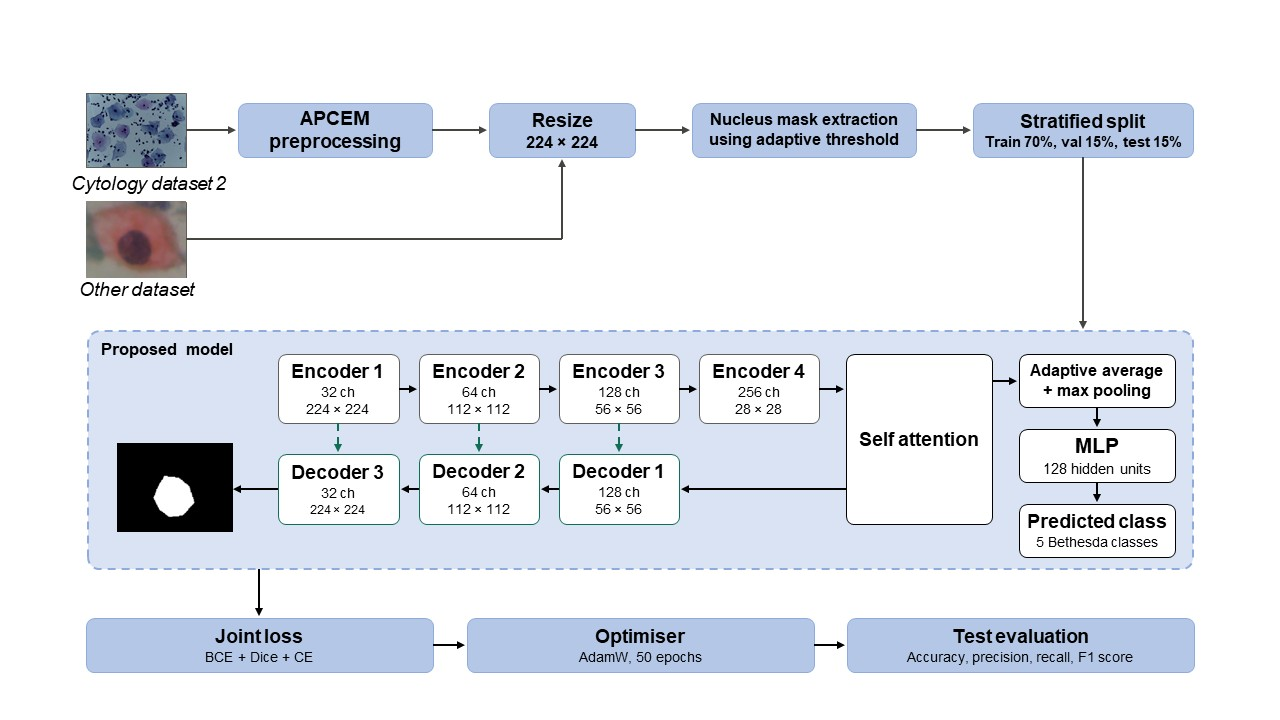
\includegraphics[width=1.0\textwidth]{image/methodology_editable (1).jpg} 
    \caption{Overall workflow of the proposed multi-task framework for cervical cell classification and nucleus segmentation.}
    \label{methodology}
\end{figure}

\subsection{Dataset}
In this study, we are performing Binary as well as Multiclass cervical cancer classification. Binary classification is to find out whether a cell is abnormal or not. If the cell is abnormal, then we need to find out the stage of cervical cell abnormality for diagnostic purposes. Thus, we are also implementing multiclass classification.

We have worked with two kind of images- 1. Pap smear image (derived from Pap smear test), 2. Cytology image (microscopic pap smear image). For pap smear image, we have used \textbf{SIPaKMeD}\cite{Lite38} dataset. And for the cytology image, we have experimented with two cervical cytology datasets—one is the \textbf{APCEM-Enhanced Cervical Cytology Image Dataset}\cite{aswini2026apcem}, and another one is \textbf{CytologCervicalCancer}\cite{jnx03_2025}. By using these two cytology image datasets, we have created a custom dataset to perform binary classification and evaluate our proposed model. 

\subsubsection{SIPaKMeD}
SIPaKMeD is a dataset for the classification of normal and pathological cervical cells in Pap smear images by using features and images. It is composed of 4049 isolated cell images, manually cropped from 966 cluster cell images of Pap smear slides, acquired by a CCD camera adapted to an optical microscope\cite{Lite38}. The cell images are distributed into five classes (Figure~\ref{sipakmed}) based on cytomorphological features containing normal, abnormal and benign cells. 
To detect the abnormality of a cell, we grouped the five classes into Normal (Superficial-Intermediate and Parabasal) and Abnormal (Koilocytotic, Dyskeratotic, and Metaplastic) for binary classification\cite{10.3389/fonc.2025.1703772}. Cell distribution as per category and class is shown in Table \ref{tab:cell_distribution}.

\begin{table}[htbp]
    \centering
    \caption{Cell Distribution of SIPAKMED dataset}
    \label{tab:cell_distribution}
    \begin{tabular}{llrl}
        \toprule
        \textbf{Category} & \textbf{Class Name} & \textbf{Cell Count} & \textbf{Description} \\
        \midrule
        Normal & Superficial-Intermediate & 813 & Healthy mature squamous cells \\
        Normal & Parabasal & 787 & Healthy deep-layer cells \\
        Abnormal & Metaplastic & 793 & Non-malignant reactive changes \\
        Abnormal & Koilocytotic & 825 & Mild dysplastic changes \\
        Abnormal & Dyskeratotic & 813 & Moderate to severe dysplasia \\
        \midrule
        \textbf{Total} & \textbf{5 Classes} & \textbf{4,049} & \textbf{} \\
        \bottomrule
    \end{tabular}
\end{table}

\begin{figure}[htbp]
    \centering
    % Image 1
    \begin{subfigure}[b]{0.19\textwidth}
        \centering
        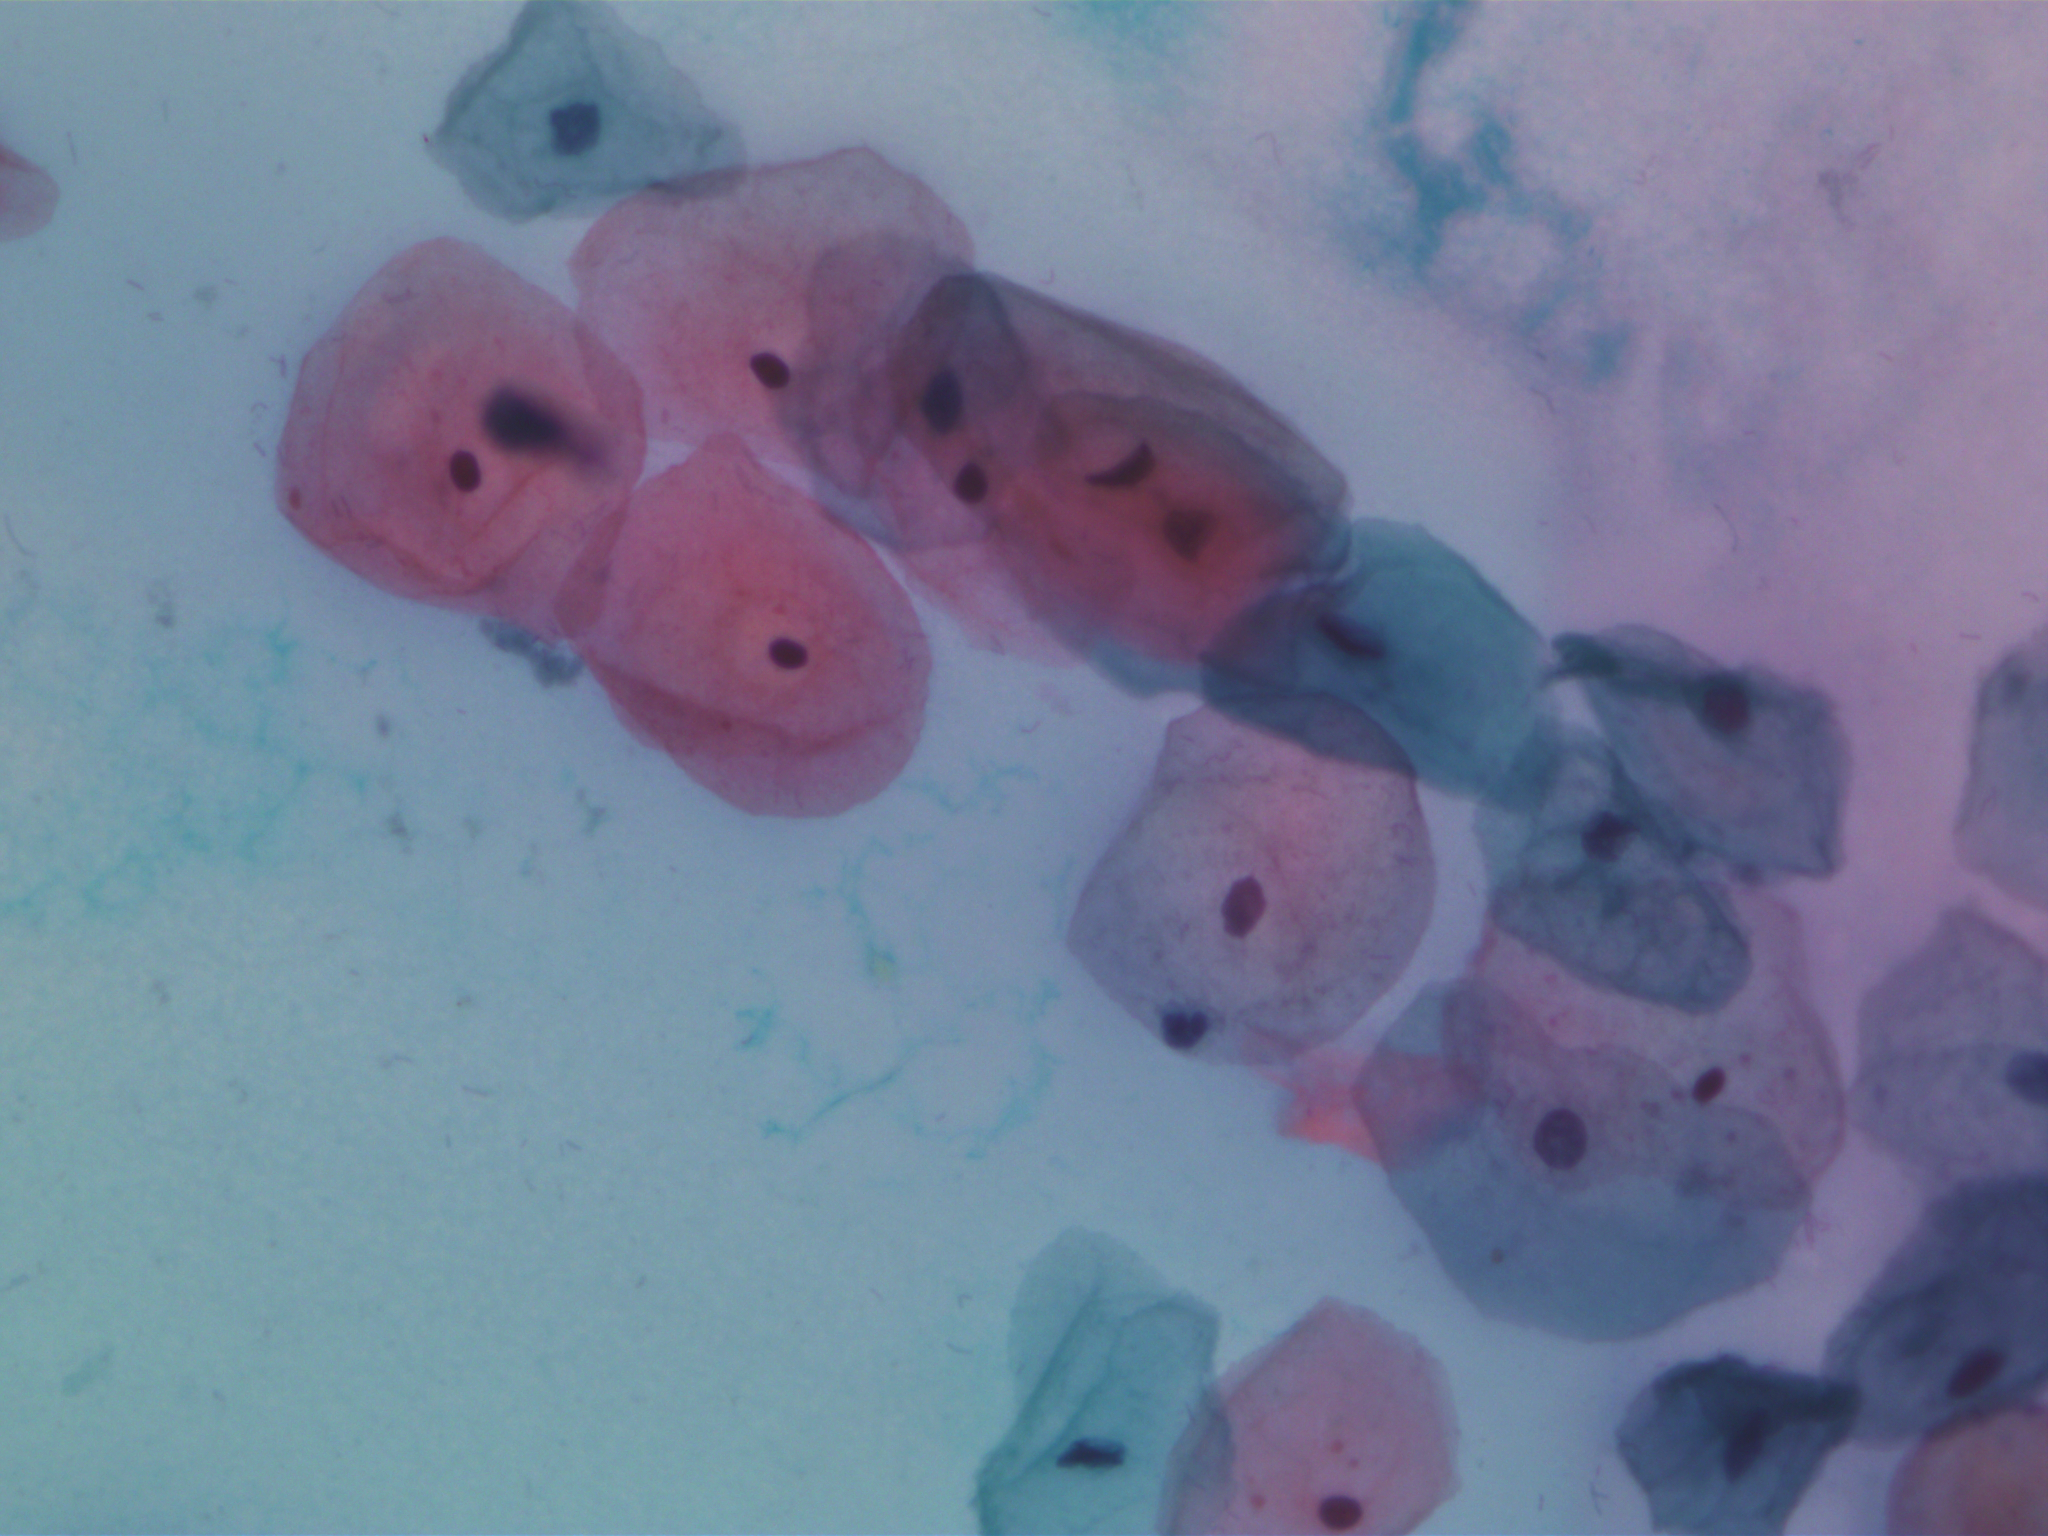
\includegraphics[width=\textwidth]{image/dataset/sipakmed/superficial1.jpg} % Replace with your image
        \caption{Superficial}
        \label{fig:img1_sipak_superficial}
    \end{subfigure}
    \hfill
    % Image 2
    \begin{subfigure}[b]{0.19\textwidth}
        \centering
        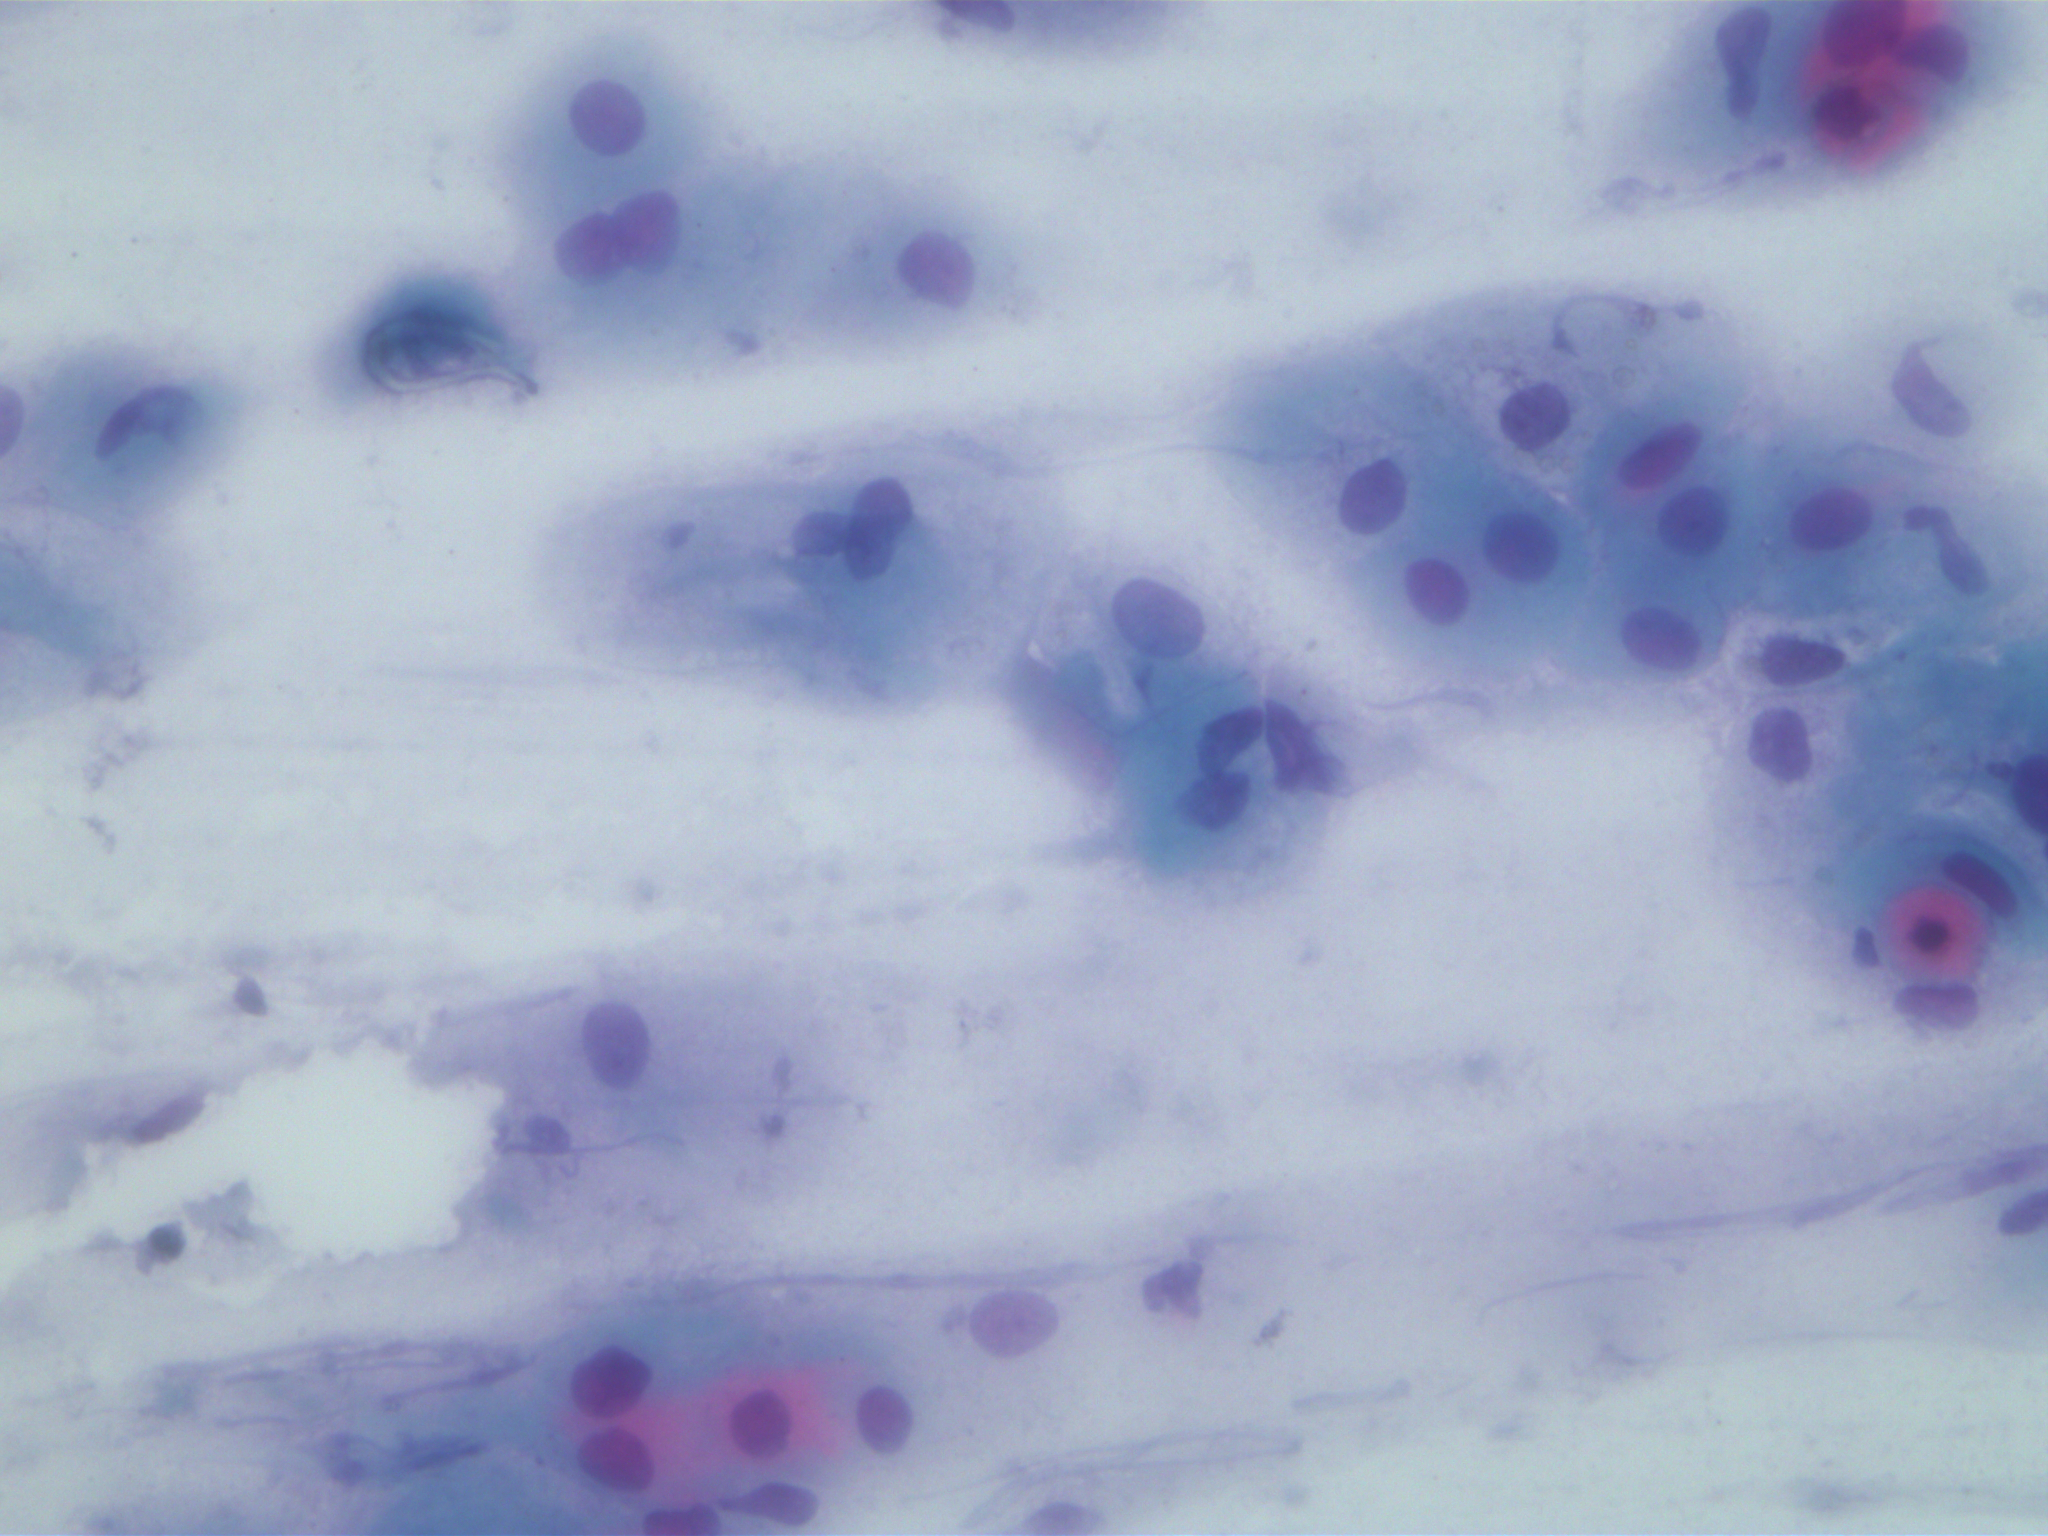
\includegraphics[width=\textwidth]{image/dataset/sipakmed/parabasal1.jpg} % Replace with your image
        \caption{Parabasal}
        \label{fig:img2_sipak_parabasal}
    \end{subfigure}
    \hfill
    % Image 3
    \begin{subfigure}[b]{0.19\textwidth}
        \centering
        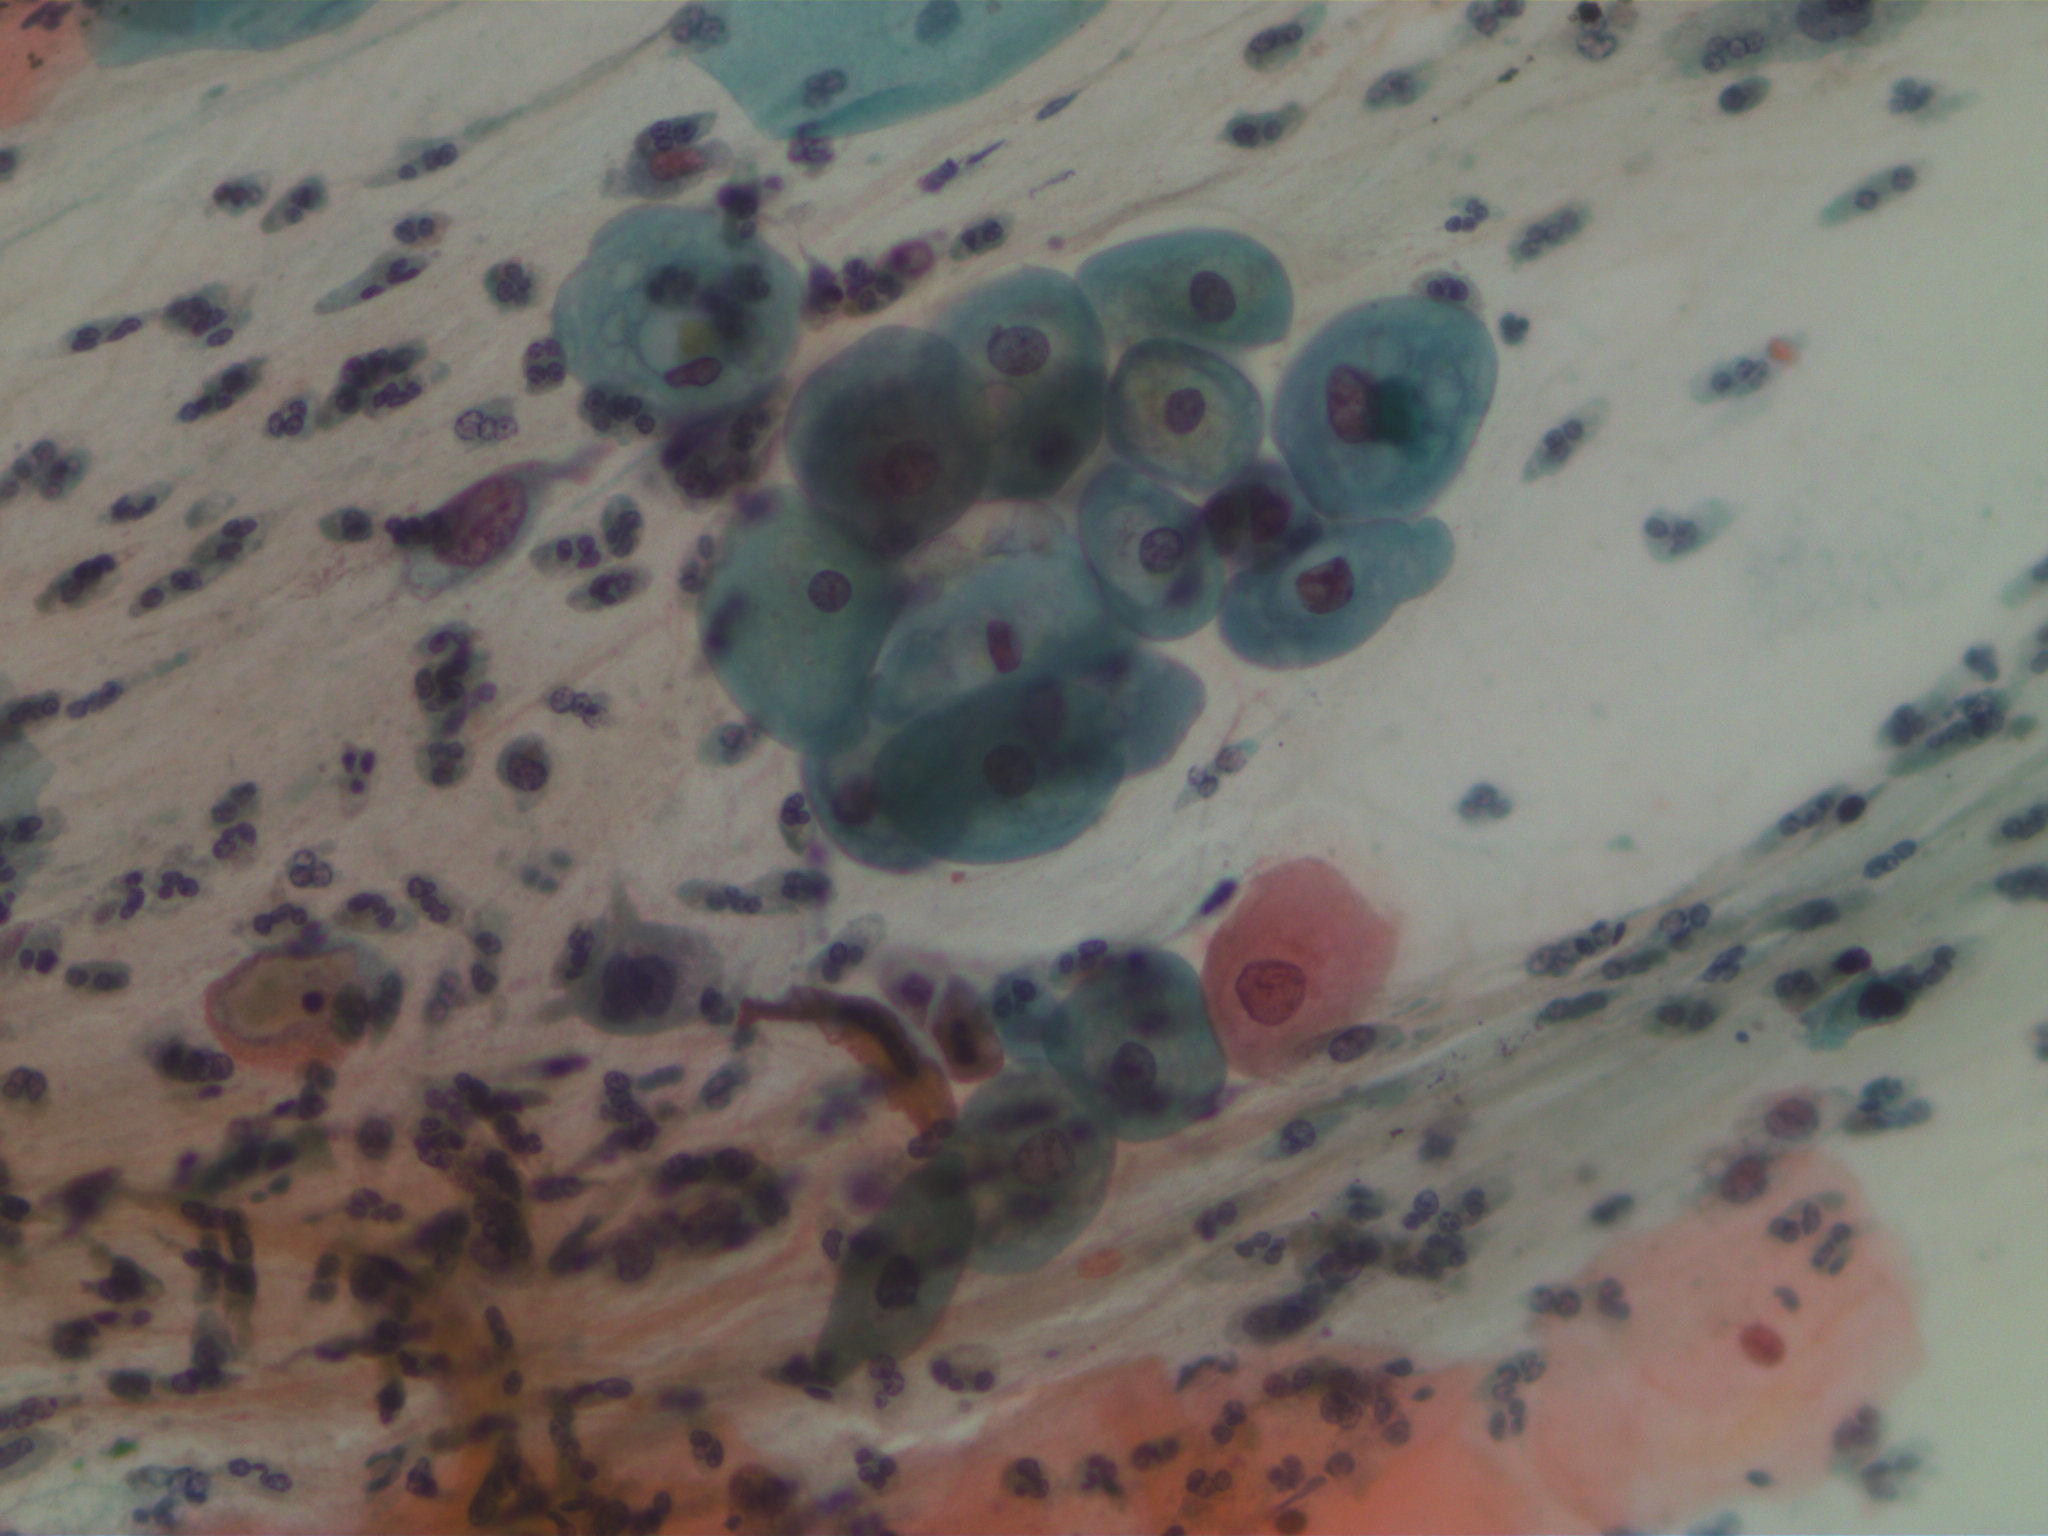
\includegraphics[width=\textwidth]{image/dataset/sipakmed/metaplastic1.jpg} % Replace with your image
        \caption{Metaplastic}
        \label{fig:img3_sipak_metaplastic}
    \end{subfigure}
    \hfill
    % Image 4
    \begin{subfigure}[b]{0.19\textwidth}
        \centering
        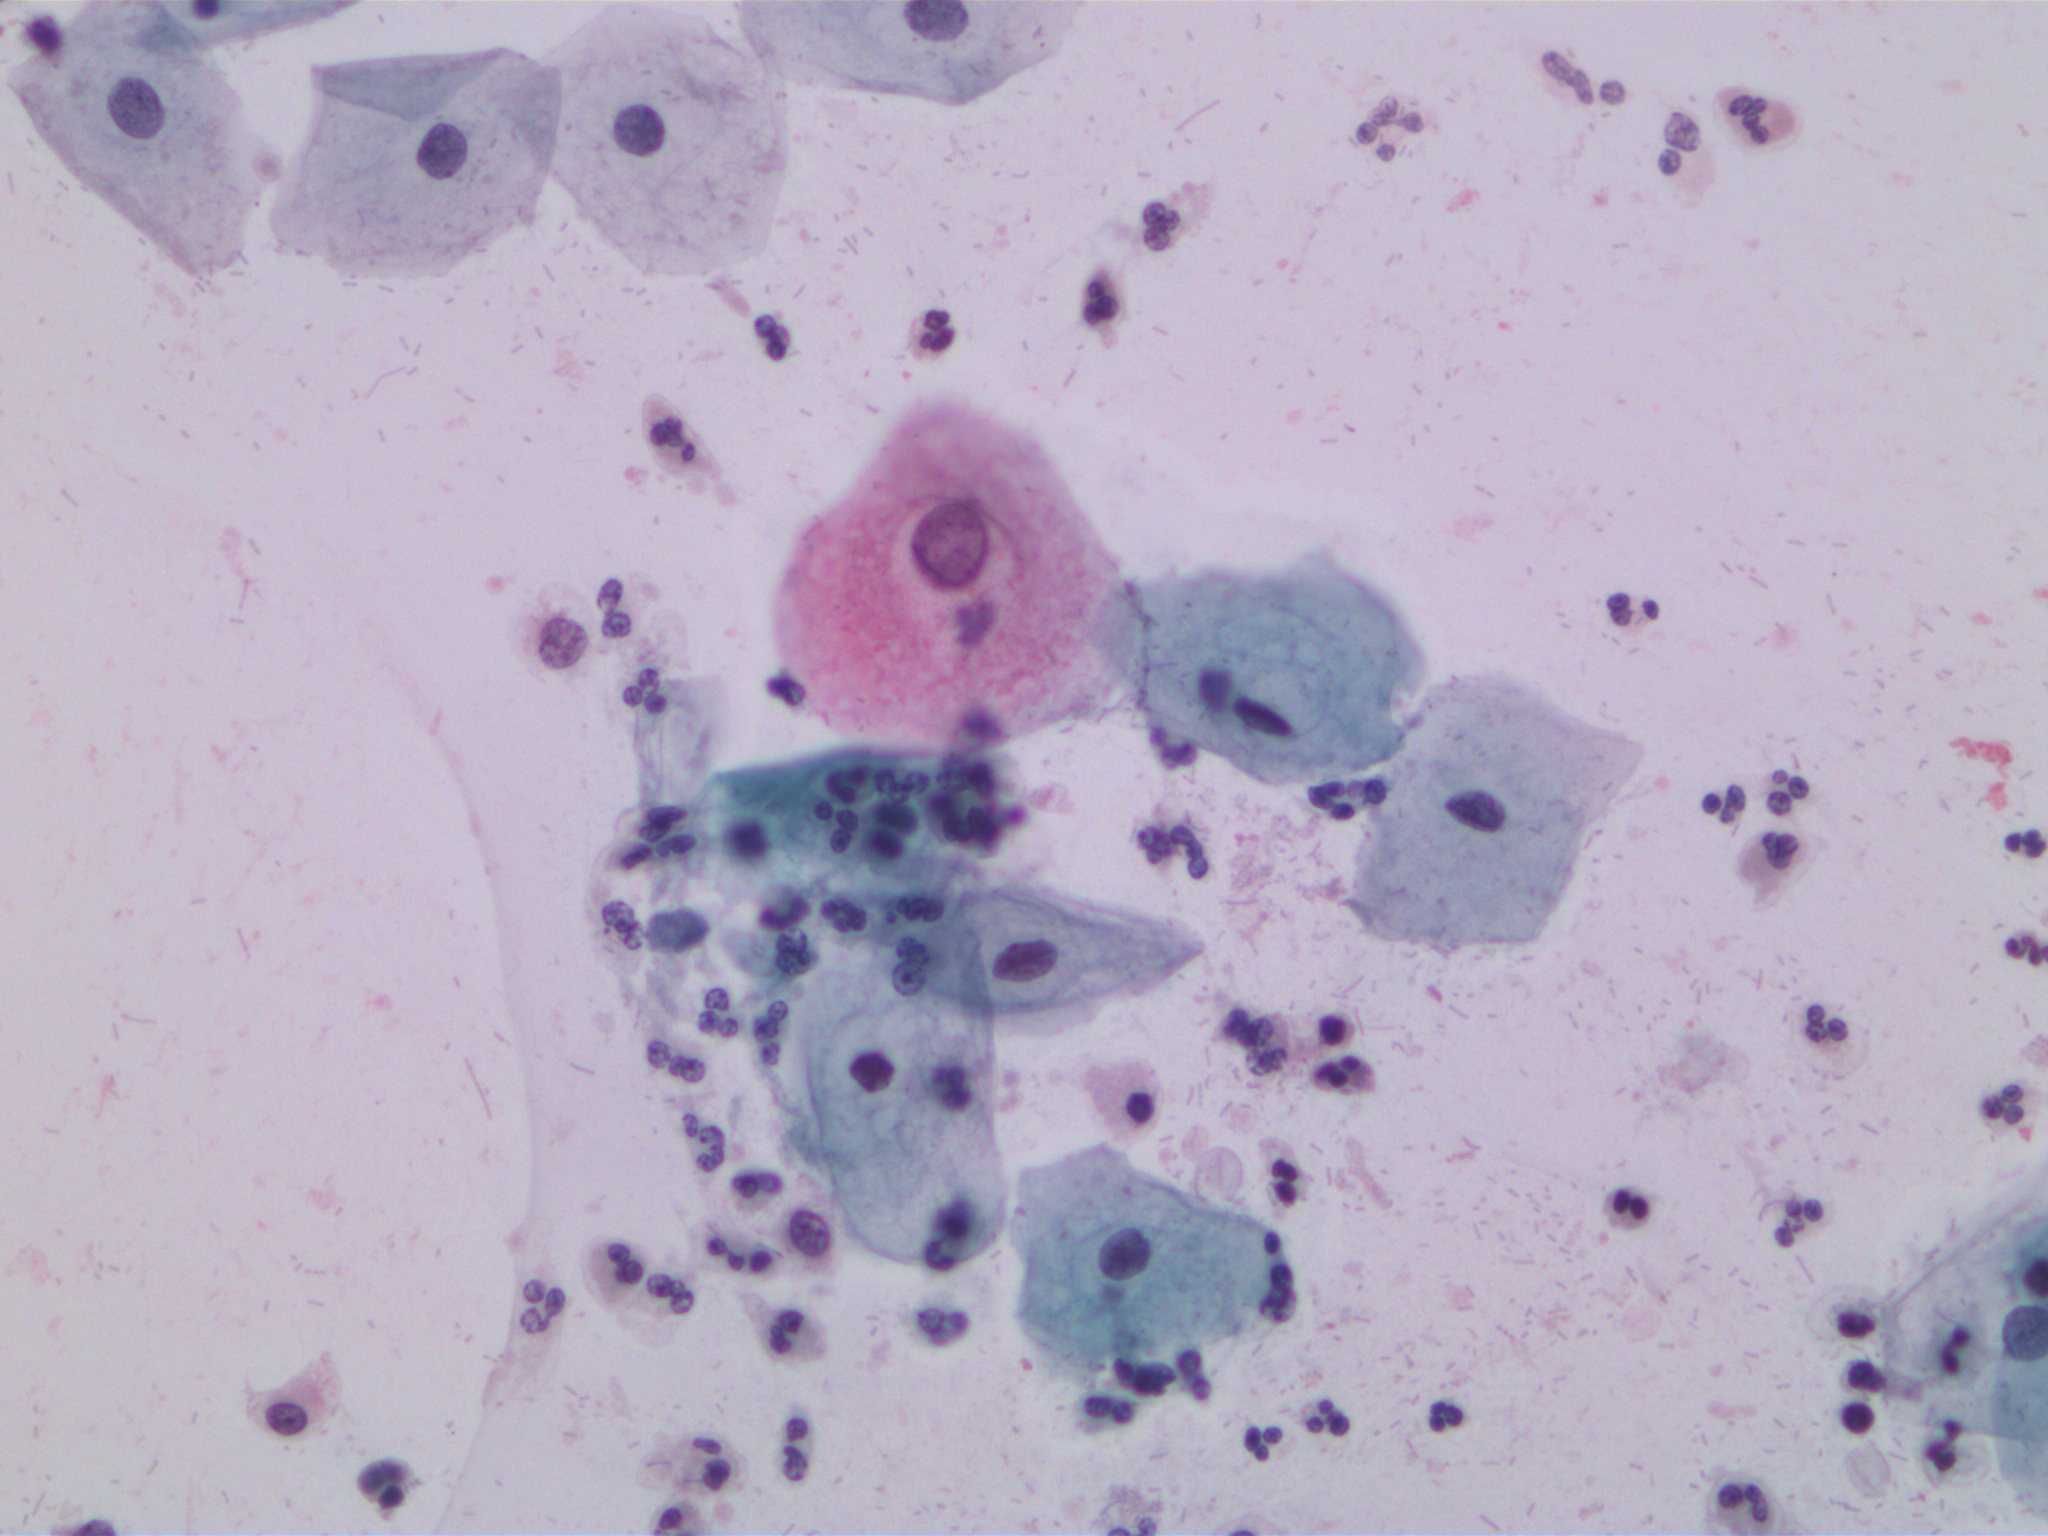
\includegraphics[width=\textwidth]{image/dataset/sipakmed/koilocytotic1.jpg} % Replace with your image
        \caption{Koilocytotic}
        \label{fig:img4_sipak_koilocytotic}
    \end{subfigure}
    \hfill
    % Image 5
    \begin{subfigure}[b]{0.19\textwidth}
        \centering
        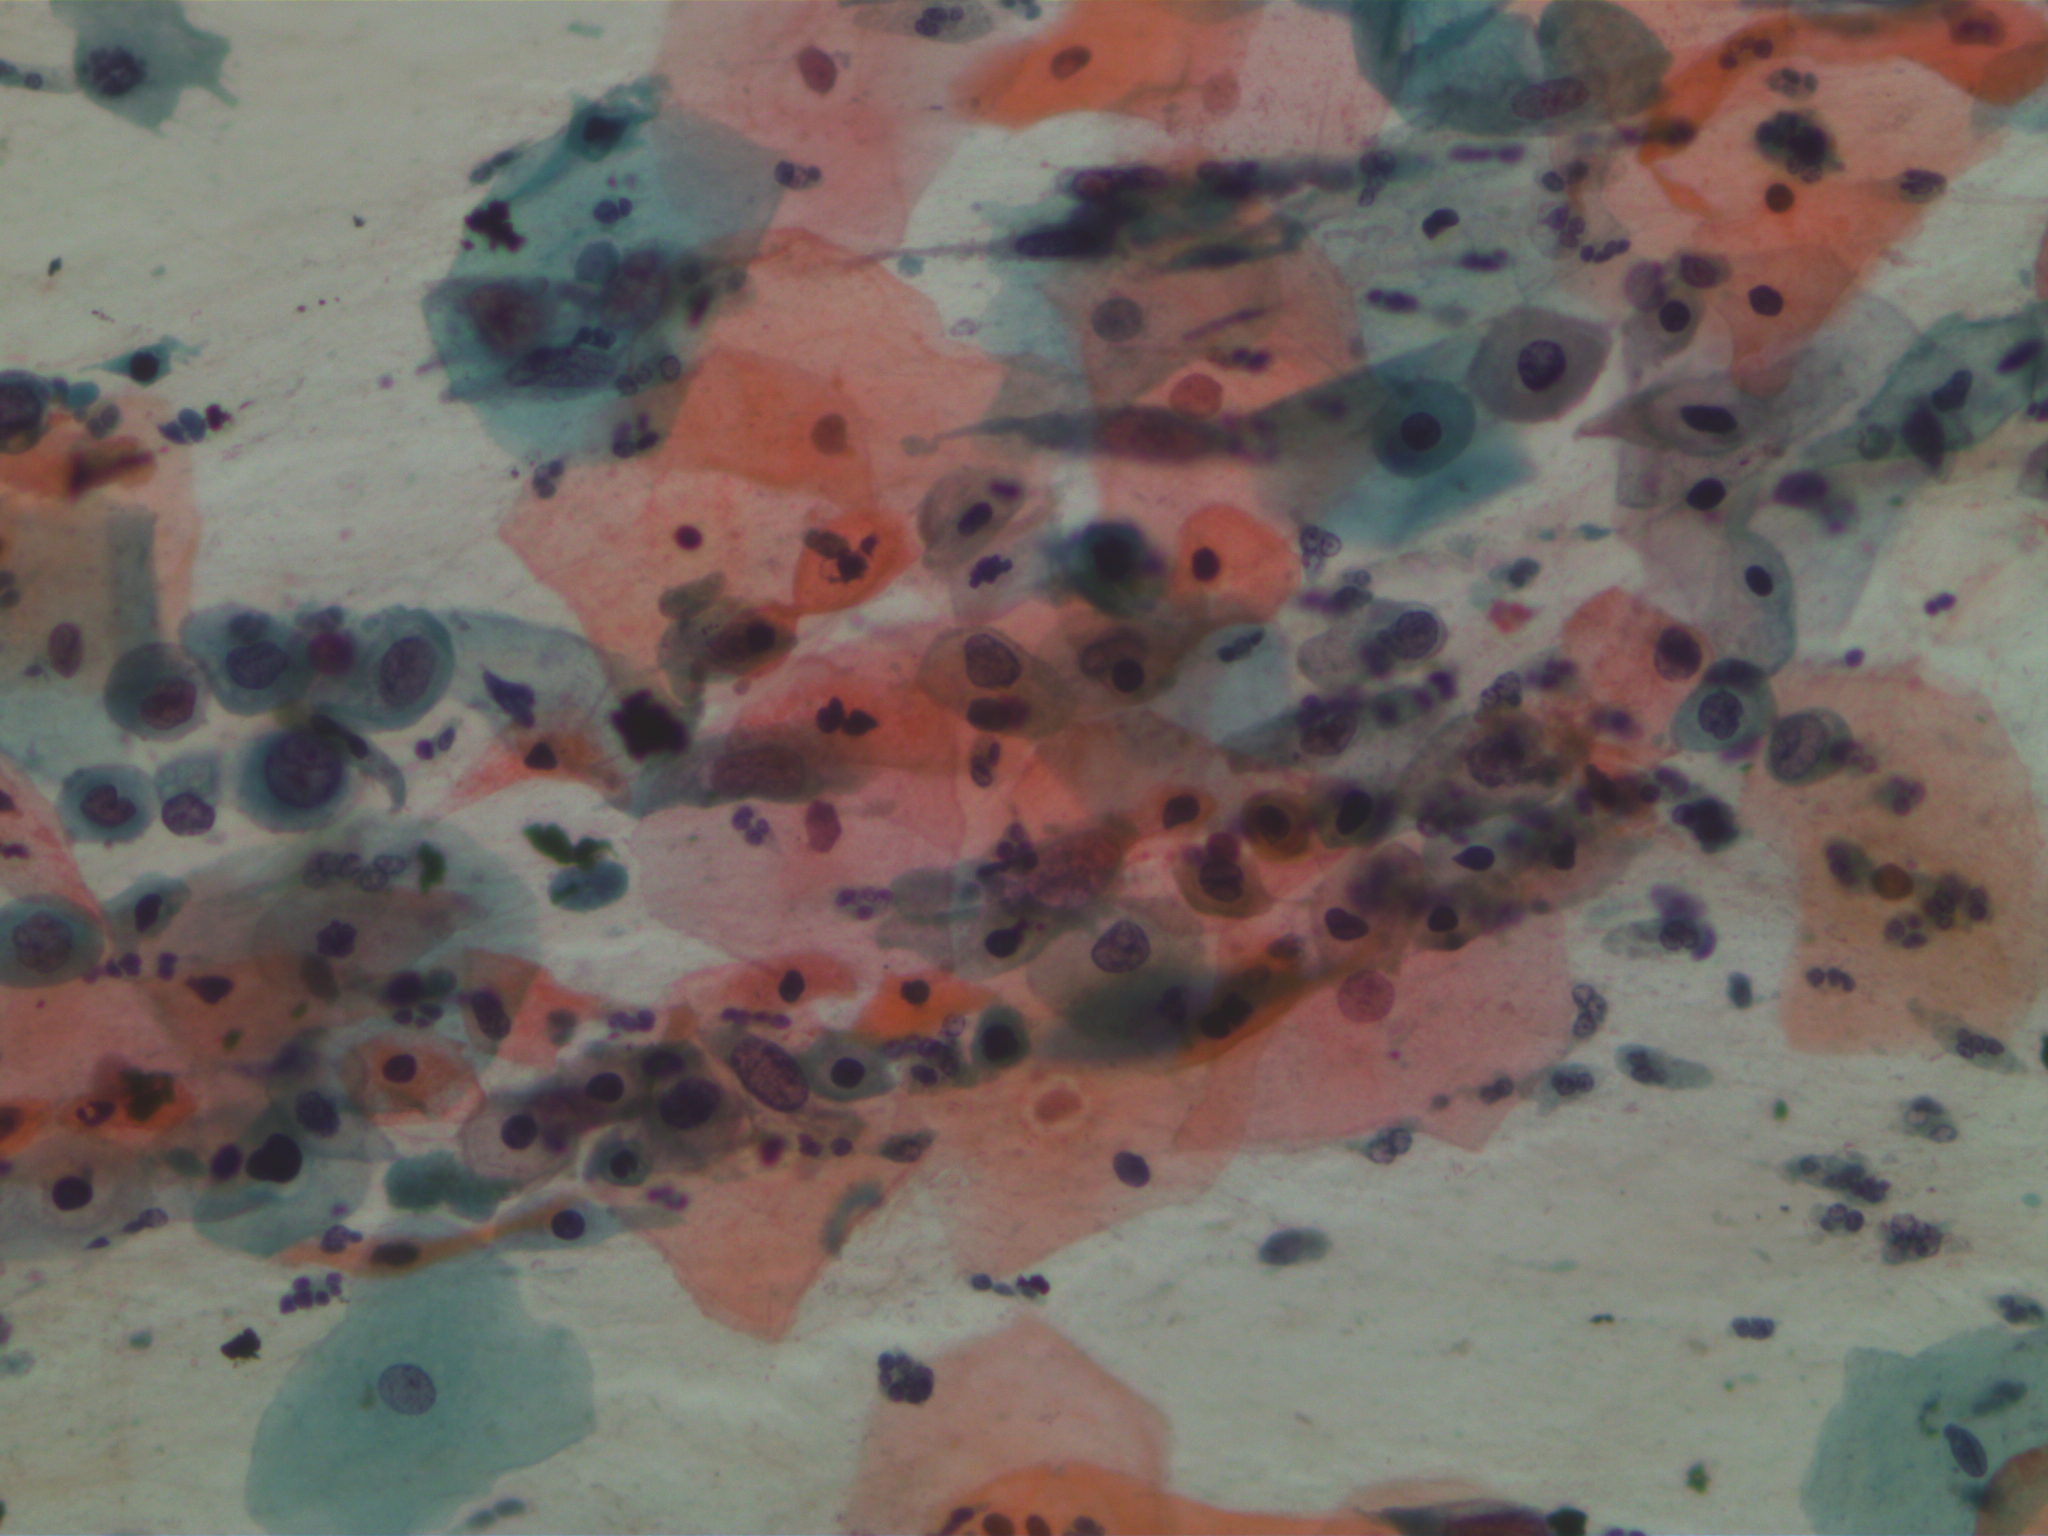
\includegraphics[width=\textwidth]{image/dataset/sipakmed/diskeratotyc1.jpg} % Replace with your image
        \caption{Dyskeratotic}
        \label{fig:img3_sipak_dyskeratotic}
    \end{subfigure}

    \caption{Visual representation of the five cellular classes of the Sipakmed dataset}
    \label{sipakmed}
\end{figure}

\subsubsection{APCEM-Enhanced Cervical Cytology Image Dataset}
The APCEM-Enhanced Cervical Cytology Image Dataset is a publicly available cervical cytology image dataset containing 4,253 Pap-smear cytology images\cite{aswini2026apcem}. This dataset is more suitable for cervical cancer detection. Because, the images were collected from cervical Pap-smear preparations under conventional imaging circumstances in the laboratory and display realistic variations in staining intensity, cellular density, cell overlap, inflammatory backdrop, mucus and debris.

The images are categorized into six clinically relevant classes according to the Bethesda System: ASCH(Atypical Squamous Cells—cannot exclude HSIL), ASCUS(Atypical Squamous Cells of Undetermined Significance), HSIL(High-Grade Squamous Intraepithelial Lesion), LSIL(Low-Grade Squamous Intraepithelial Lesion), NILM(Negative for Intraepithelial Lesion or Malignancy), and SCC(Squamous Cell Carcinoma). This dataset has only 119 ASCH cell images, whereas our another cytology dataset don't even have this class. So, to have a better comparative analysis and to minimize class imbalance, we exclude 119 ASCH images and experiment with 4134 images.
Cell distribution as per category and class is shown in
Table~\ref{tab:cell_distribution_APCEM}. Figure~\ref{cytology1} represents a sample image of each class.

\begin{table}[htbp]
    \centering
    \caption{Cell Distribution of APCEM-Enhanced Cervical Cytology Image Dataset}
    \label{tab:cell_distribution_APCEM}
    \begin{tabular}{llrl}
        \toprule
        \textbf{Category} & \textbf{Class Name} & \textbf{Cell Count} & \textbf{Description} \\
        \midrule
        Normal   & NILM  & 779 & Negative for intraepithelial lesion or malignancy \\
        Abnormal & ASCUS & 340 & Atypical squamous cells of undetermined significance \\
        Abnormal & HSIL  & 1,300 & High-grade squamous intraepithelial lesion \\
        Abnormal & LSIL  & 1,241 & Low-grade squamous intraepithelial lesion \\
        Abnormal & SCC   & 474 & Squamous cell carcinoma \\
        \midrule
        \textbf{Total} & \textbf{5 Classes} & \textbf{4,134} & \\
        \bottomrule
    \end{tabular}
\end{table}

\begin{figure}[htbp]
    \centering
    % Image 1
    \begin{subfigure}[b]{0.19\textwidth}
        \centering
        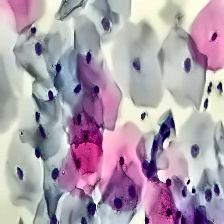
\includegraphics[width=\textwidth]{image/dataset/cytology1/NILM_01 (45).jpg} % Replace with your image
        \caption{NILM}
        \label{fig:img1_apcem_enh_nilm}
    \end{subfigure}
    \hfill
    % Image 2
    \begin{subfigure}[b]{0.19\textwidth}
        \centering
        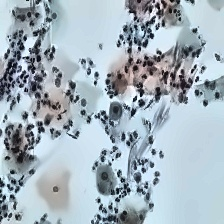
\includegraphics[width=\textwidth]{image/dataset/cytology1/ASC_US_01 (16).jpg} % Replace with your image
        \caption{ASCUS}
        \label{fig:img1_apcem_enh_ascus}
    \end{subfigure}
    \hfill
    % Image 3
    \begin{subfigure}[b]{0.19\textwidth}
        \centering
        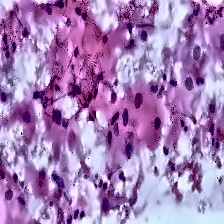
\includegraphics[width=\textwidth]{image/dataset/cytology1/HSIL_01 (20).jpg} % Replace with your image
        \caption{HSIL}
        \label{fig:img1_apcem_enh_hsil}
    \end{subfigure}
    \hfill
    % Image 4
    \begin{subfigure}[b]{0.19\textwidth}
        \centering
        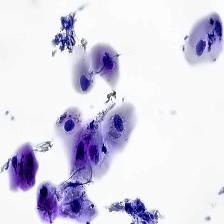
\includegraphics[width=\textwidth]{image/dataset/cytology1/LSIL_01 (12).jpg} % Replace with your image
        \caption{LSIL}
        \label{fig:img1_apcem_enh_lsil}
    \end{subfigure}
    \hfill
    % Image 5
    \begin{subfigure}[b]{0.19\textwidth}
        \centering
        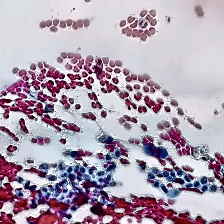
\includegraphics[width=\textwidth]{image/dataset/cytology1/SCC_01 (56).jpg} % Replace with your image
        \caption{SCC}
        \label{img1_apcem_enh_scc}
    \end{subfigure}

    \caption{Visual representation of the five cellular classes of the APCEM-Enhanced Cervical Cytology Image Dataset}
    \label{cytology1}
\end{figure}



\subsubsection{CytologCervicalCancer}

The CytologCervicalCancer dataset is a curated cervical cytology image dataset gathered from researchers and cancer hospitals worldwide\cite{jnx03_2025}. Main motivation behind constructing this dataset was to provide a high-quality, regionally representative image set for training machine-learning models on pre-cancerous and cancerous cervical cell detection.

It has total 2634 images catergorized into 5 classes. The classes are normal to pre-cancerous to cancerous stage namely- ASCUS, HSIL, LSIL, NILM, SCC (Figure \ref{cytology2}). We preprocessed the CytologCervicalCancer dataset using the APCEM framework to assess its effectiveness and to ensure a fair comparison across identical five-class categories. Cell distribution as per category and class is shown in Table~\ref{tab:cell_distribution_cytolog}.

\begin{table}[htbp]
    \centering
    \caption{Cell Distribution of CytologCervicalCancer Dataset}
    \label{tab:cell_distribution_cytolog}
    \begin{tabular}{llrl}
        \toprule
        \textbf{Category} & \textbf{Class Name} & \textbf{Cell Count}  \\
        \midrule
        Normal   & NILM  & 612  \\
        Abnormal & ASCUS & 198  \\
        Abnormal & HSIL  & 845 \\
        Abnormal & LSIL  & 613  \\
        Abnormal & SCC   & 366  \\
        \midrule
        \textbf{Total} & \textbf{5 Classes} & \textbf{2,634} & \\
        \bottomrule
    \end{tabular}
\end{table}

\begin{figure}[htbp]
    \centering
    % Image 1
    \begin{subfigure}[b]{0.19\textwidth}
        \centering
        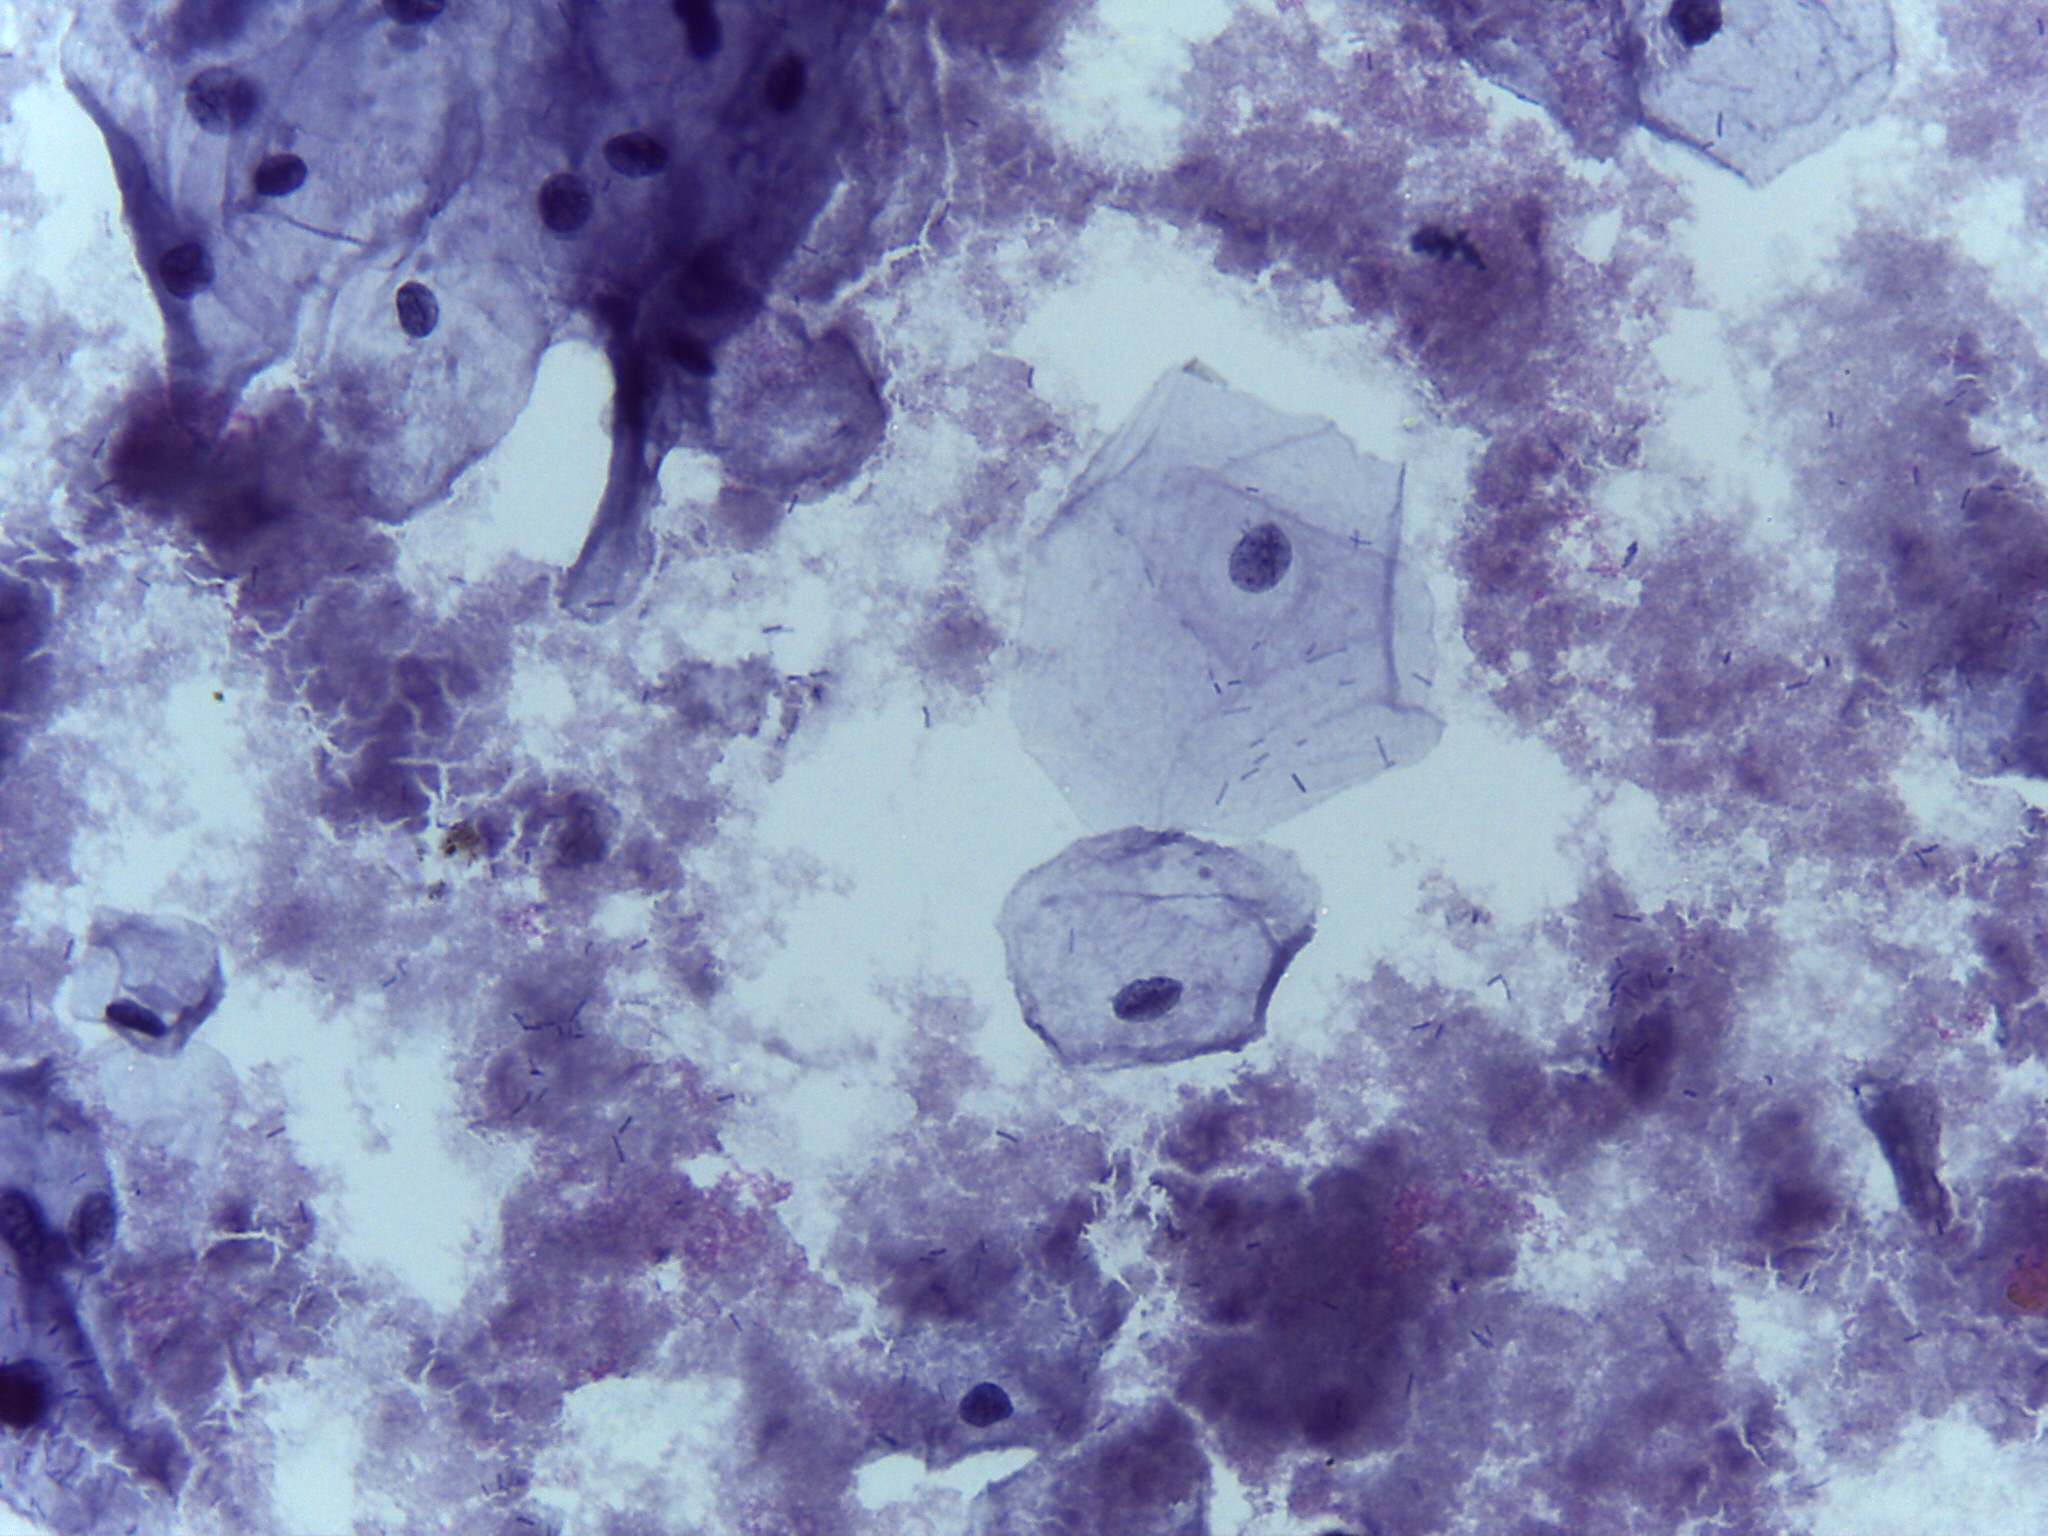
\includegraphics[width=\textwidth]{image/dataset/cytology2/NL_13_ (6).jpg} % Replace with your image
        \caption{NILM}
        \label{fig:img1_cytolog_nilm}
    \end{subfigure}
    \hfill
    % Image 2
    \begin{subfigure}[b]{0.19\textwidth}
        \centering
        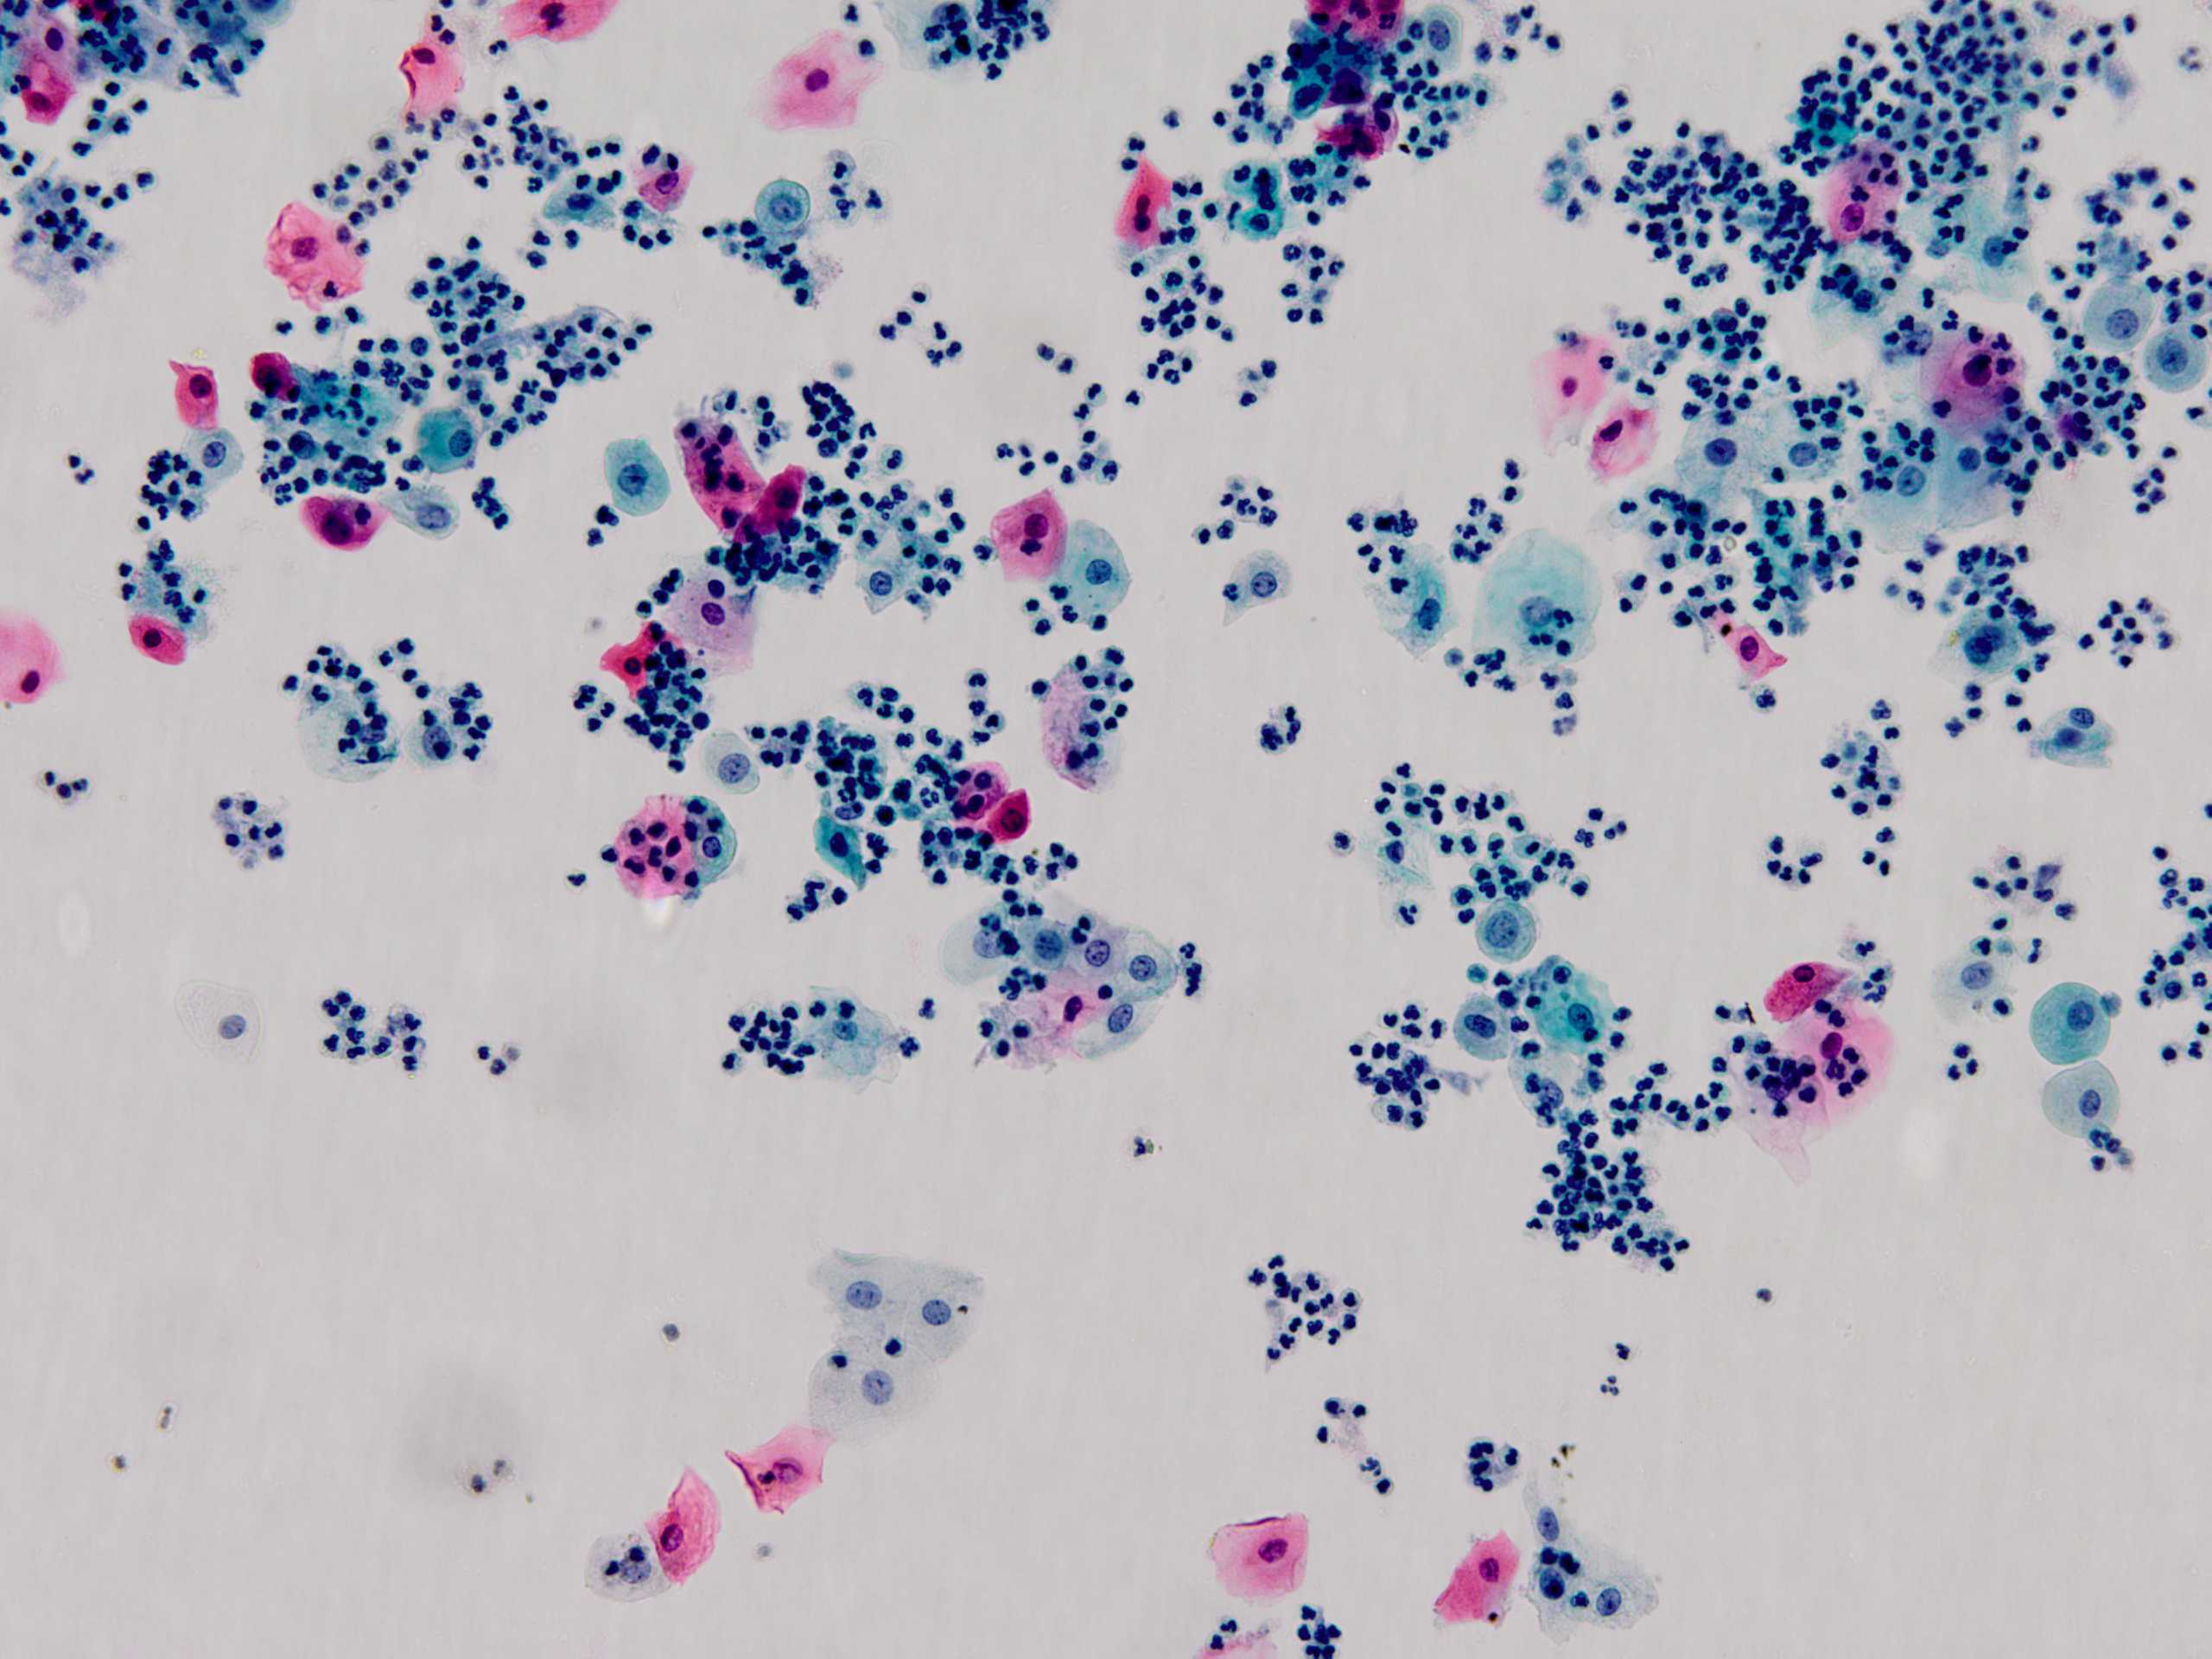
\includegraphics[width=\textwidth]{image/dataset/cytology2/A005x20D302.jpg} % Replace with your image
        \caption{ASCUS}
        \label{fig:img1_cytolog_ascus}
    \end{subfigure}
    \hfill
    % Image 3
    \begin{subfigure}[b]{0.19\textwidth}
        \centering
        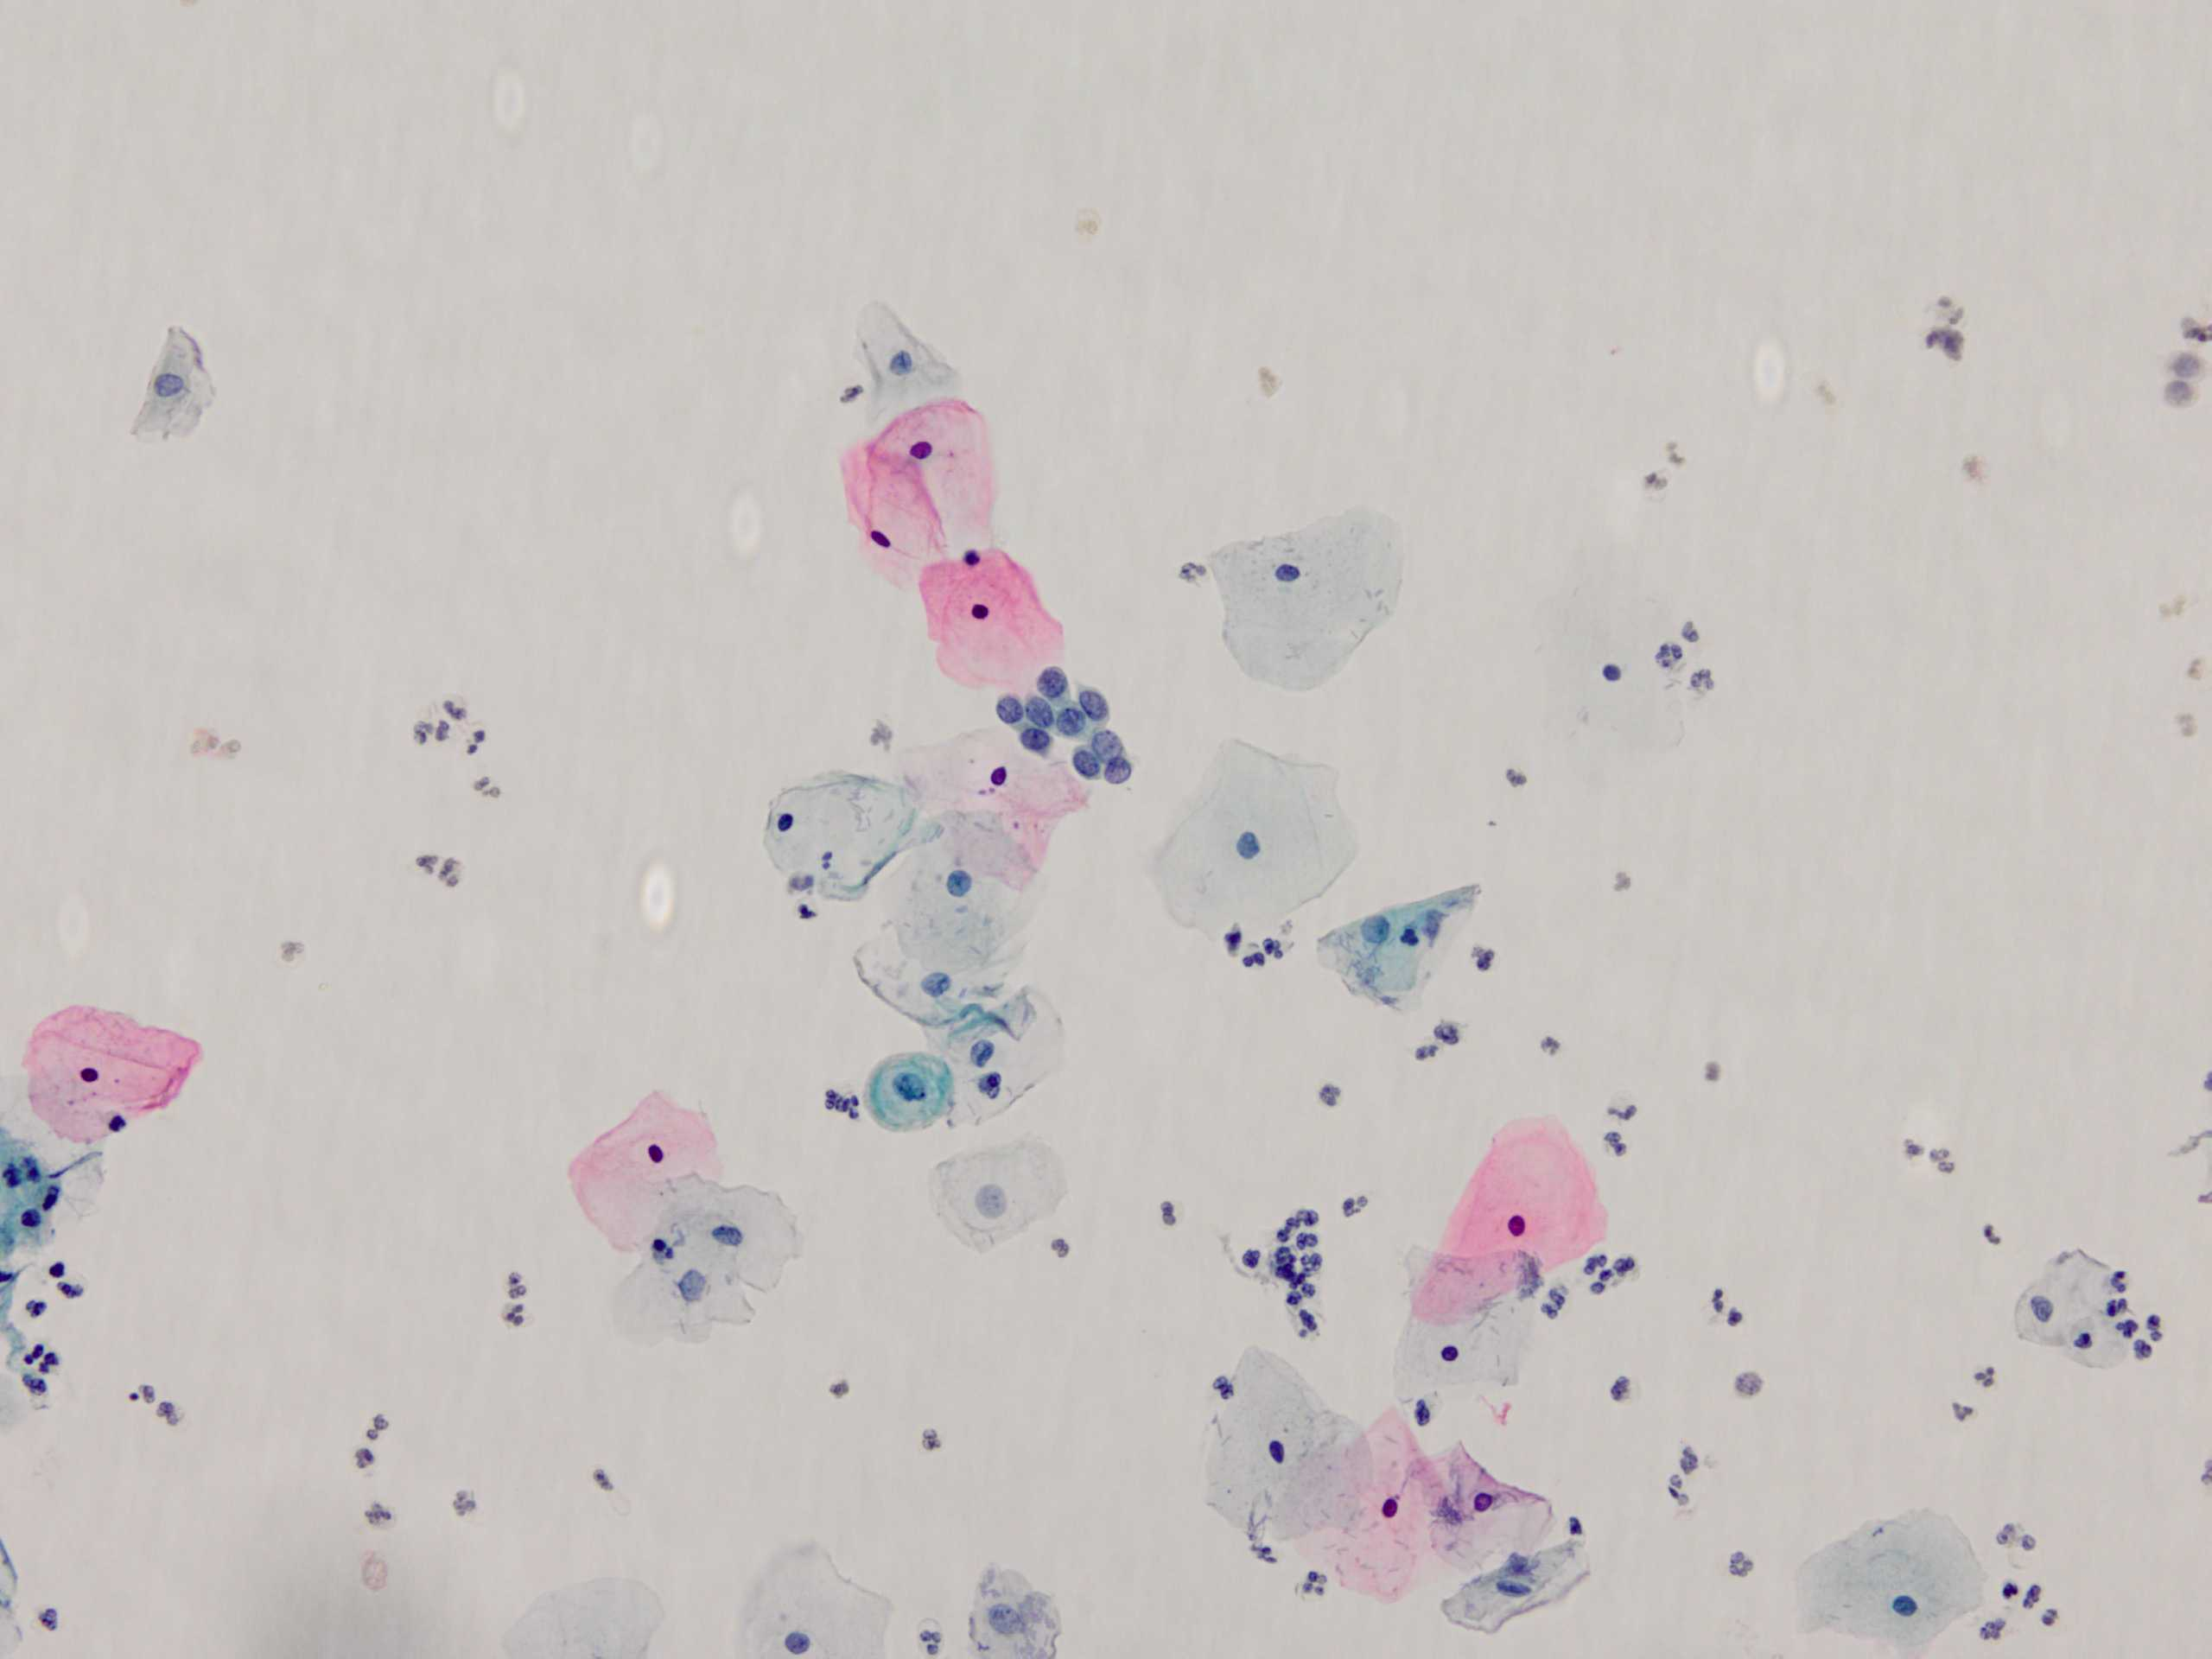
\includegraphics[width=\textwidth]{image/dataset/cytology2/H001D8x20064.jpg} % Replace with your image
        \caption{HSIL}
        \label{fig:img1_cytolog_hsil}
    \end{subfigure}
    \hfill
    % Image 4
    \begin{subfigure}[b]{0.19\textwidth}
        \centering
        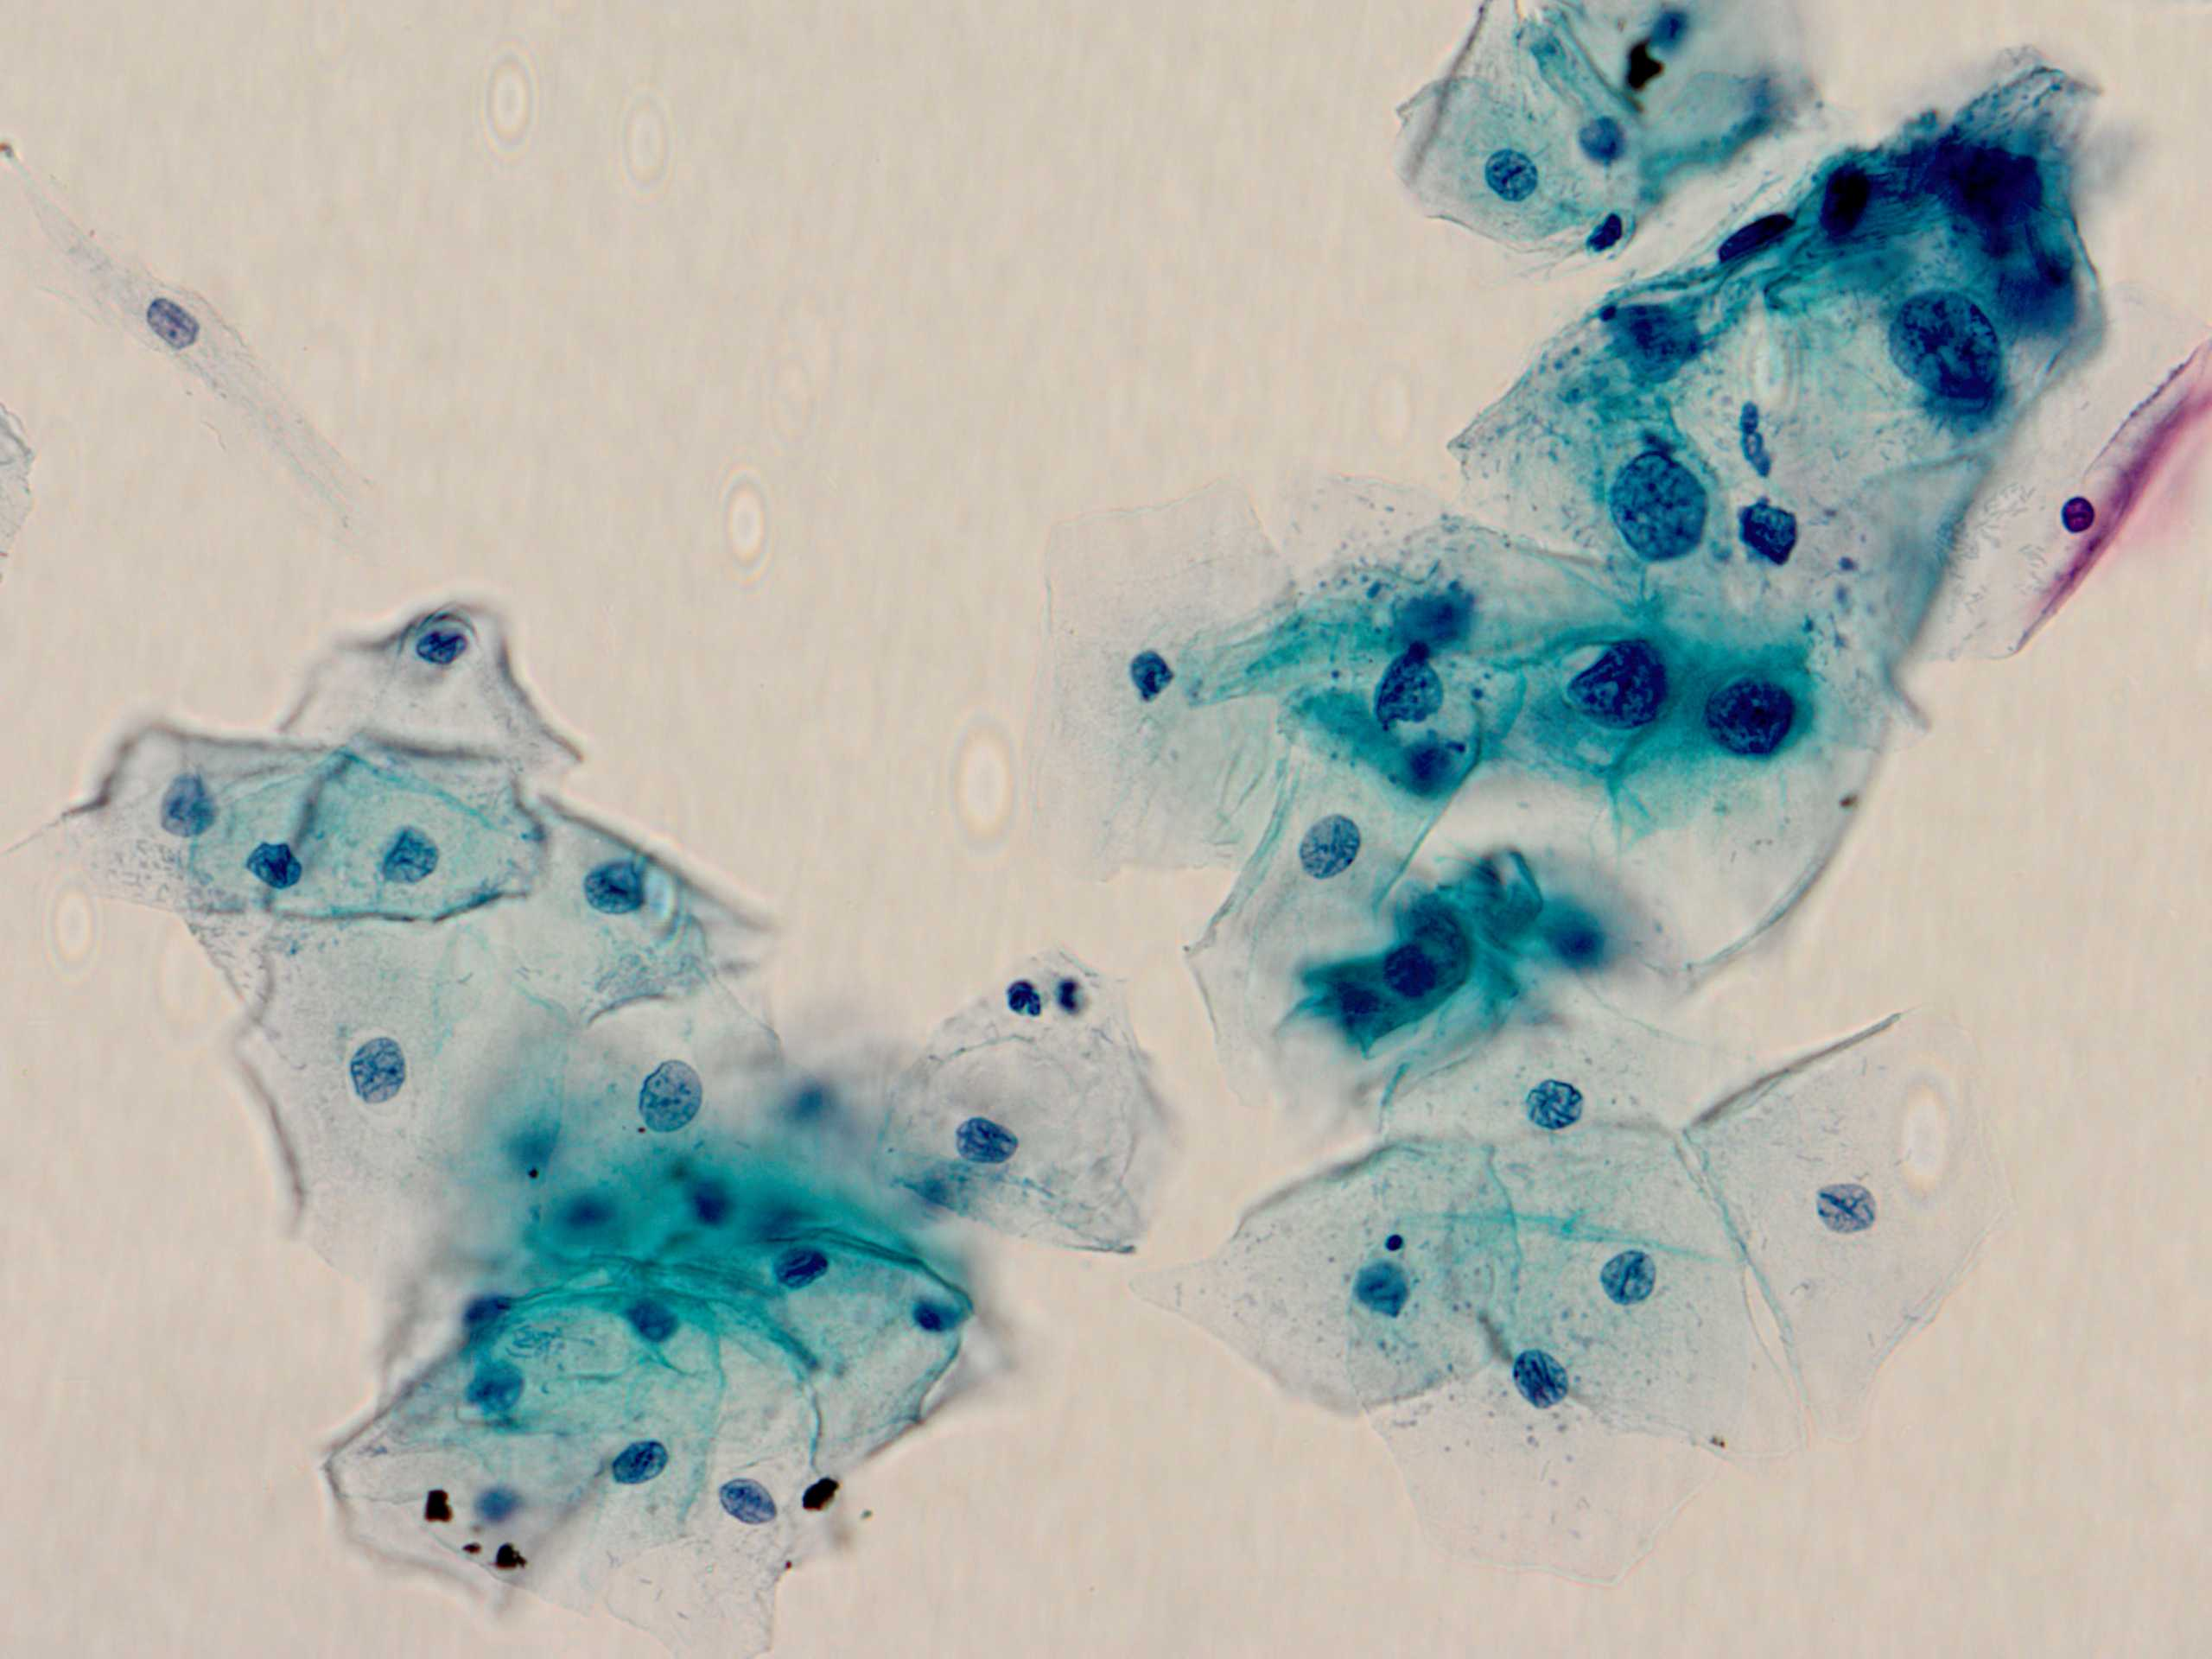
\includegraphics[width=\textwidth]{image/dataset/cytology2/L002C1x40011.jpg} % Replace with your image
        \caption{LSIL}
        \label{fig:img1_cytolog_lsil}
    \end{subfigure}
    \hfill
    % Image 5
    \begin{subfigure}[b]{0.19\textwidth}
        \centering
        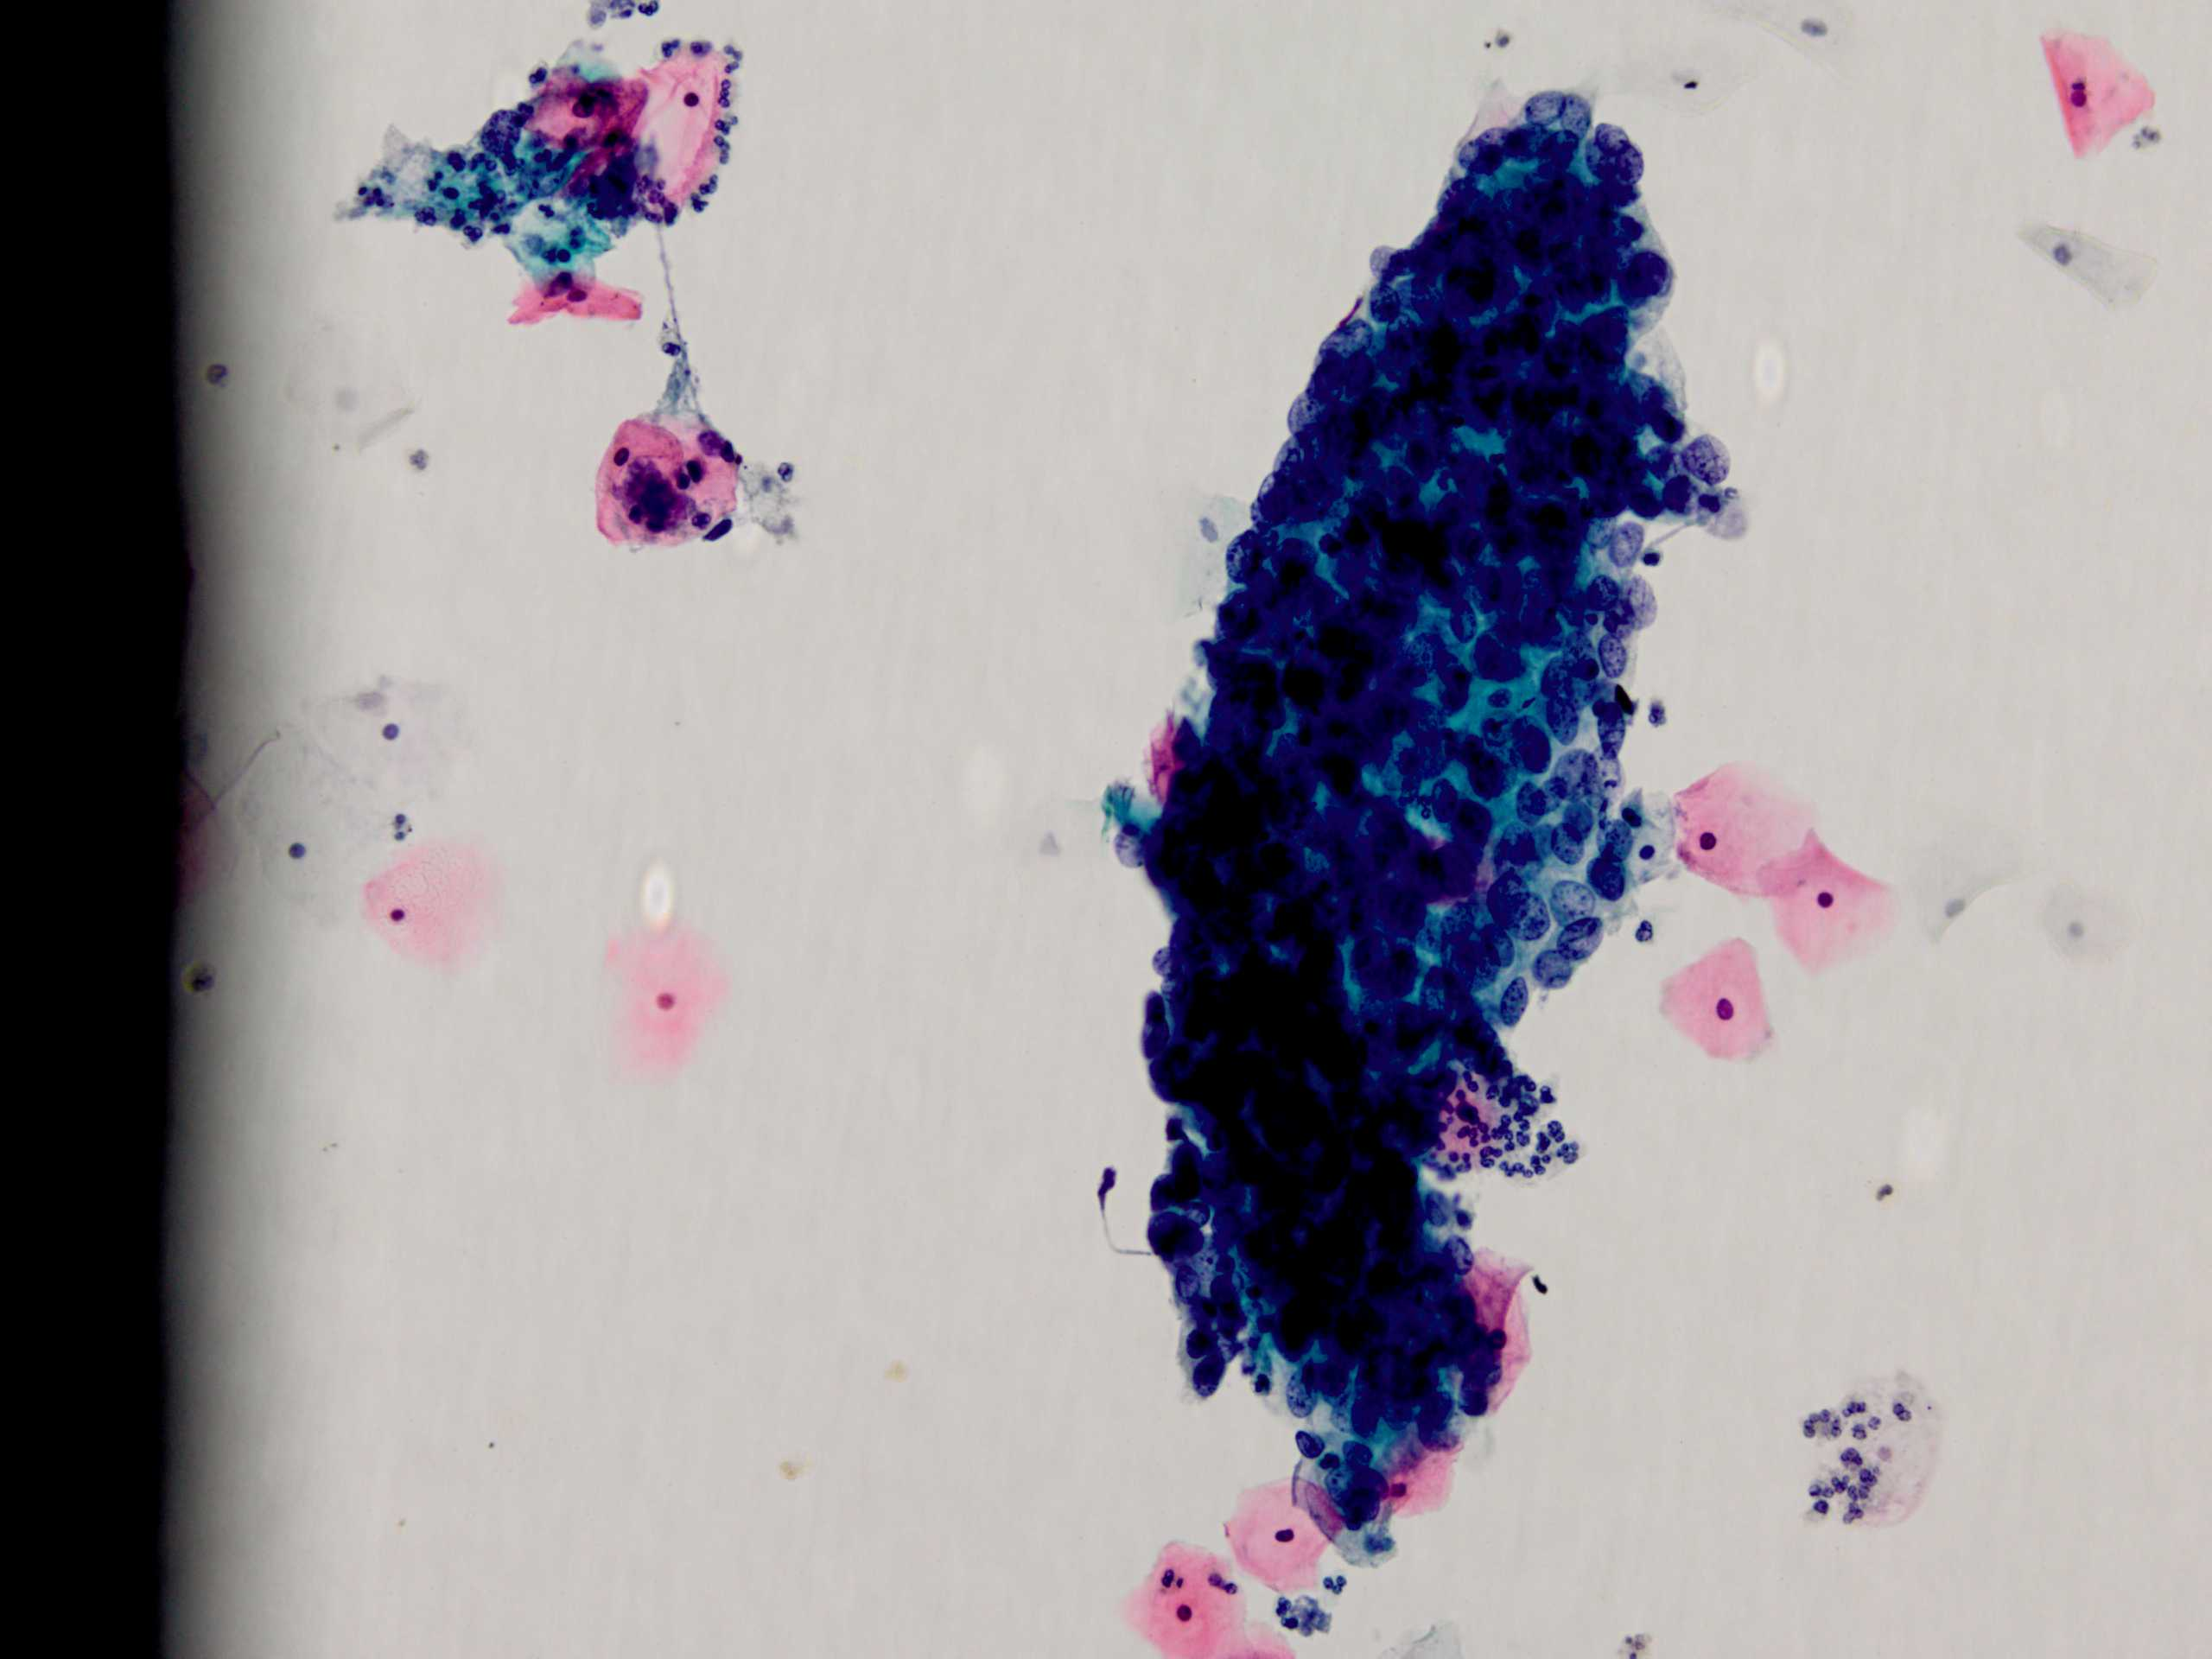
\includegraphics[width=\textwidth]{image/dataset/cytology2/scc.jpg} % Replace with your image
        \caption{SCC}
        \label{img1_cytolog_scc}
    \end{subfigure}

    \caption{Visual representation of the five cellular classes of the CytologCervicalCancer Dataset}
    \label{cytology2}
\end{figure}

\subsubsection{Custom Cervical Cytology Dataset}

For medical image dataset it's very important to have variations; otherwise, the model is trained on dataset-specific visual characteristics rather than robust features. Thus, we constructed a custom cervical cytology dataset by combining all images from the publicly available APCEM-Enhanced Cervical Cytology Image Dataset and the CytologCervicalCancer dataset to increase the diversity and scale of the available training data with a unified class structure. The resultant dataset offers a wider variety of staining properties, cell appearances, image acquisition conditions, and morphological differences than either dataset individually.

For consistency across the two source datasets, the images were reorganized according to a common class structure. For multi-class classification, the dataset is organized as-NILM, ASCUS, LSIL, HSIL, and SCC. Images belonging to same diagnostic categories were merged into the same class, whereas categories that were not common to both datasets, such as ASCH, were omitted from the unified five-class categorization setting.

Due to varying image counts across categories, the initial dataset suffered from class imbalance, which adversely impacts model training performance. To mitigate this issue and establish a balanced binary classification dataset, we reorganized the data into two primary categories: Normal class consisting of NILM samples and Abnormal class formed by merging LSIL, HSIL, and SCC samples. As the number of samples in NILM class is less, we merged all the images from both the datasets. Conversely, for the abnormal class, clear nuclear boundaries, minimal stain, high-quality images were selectively curated under the expert guidance of a medical doctor. Cell distribution as per category and class for Binary and Multi-class classification is shown in Table~\ref{tab:binary_distribution} and \ref{tab:multiclass_distribution}.

\begin{table*}[htbp]
\centering

\begin{minipage}[t]{\textwidth}
\centering
\caption{Class Distribution for Binary Classification}
\label{tab:binary_distribution}
\begin{tabular}{llr}
\toprule
\textbf{Category} & \textbf{Class Name} & \textbf{Cell Count} \\
\midrule
Normal   & NILM & 1,391 \\
Abnormal & LSIL + HSIL + SCC & 1,391 \\
\midrule
\textbf{Total} & \textbf{2 Classes} & \textbf{2,782} \\
\bottomrule
\end{tabular}
\end{minipage} \\

\begin{minipage}[t]{\textwidth}
\centering
\caption{Class Distribution for Multiclass Classification}
\label{tab:multiclass_distribution}
\begin{tabular}{llr}
\toprule
\textbf{Class Name} & \textbf{Cell Count} \\
\midrule
NILM  & 1,391 \\
ASCUS & 538 \\
HSIL  & 2,145 \\
LSIL  & 1,854 \\
SCC   & 840 \\
\midrule
\textbf{Total} & \textbf{6,768} \\
\bottomrule
\end{tabular}
\end{minipage}
\hfill 

\end{table*}

The combined dataset was developed not merely to increase the number of images, but to provide a more heterogeneous and challenging benchmark for evaluating the robustness of the proposed deep learning framework. The use of images originating from different datasets enables the model to learn more generalizable cytological representations and provides a stronger basis for assessing its performance under variations in image characteristics and data distribution.

\subsection{Pre-processing Technique}
\subsubsection{APCEM Model}
The Dataset\cite{aswini2026apcem} used APCEM model to enhance the cell structures. But the dataset\cite{jnx03_2025} consists of pure raw image. So to have a better comparative analysis, we pre-processed the images of CytologCervicalCancer\cite{jnx03_2025} with APCEM model. 

The Adaptive Parameterized Cytology Enhancement Model (APCEM), a deterministic, non-learning-based image enhancement pipeline, was used to improve the images. It enhanced cellular visibility while maintaining nuclear and cytoplasmic structures that are relevant for diagnosis shown in Figure~\ref{apcem}. The APCEM pipeline includes:

\begin{itemize}
    \item \textbf{Spatial resolution normalization:} At first, images were resized to a uniform resolution of 224 × 224 pixels. And then images were converted to the 8-bit intensity range [0,255] to have OpenCV-compatible images.  

    \begin{figure}[htbp]
    \centering
    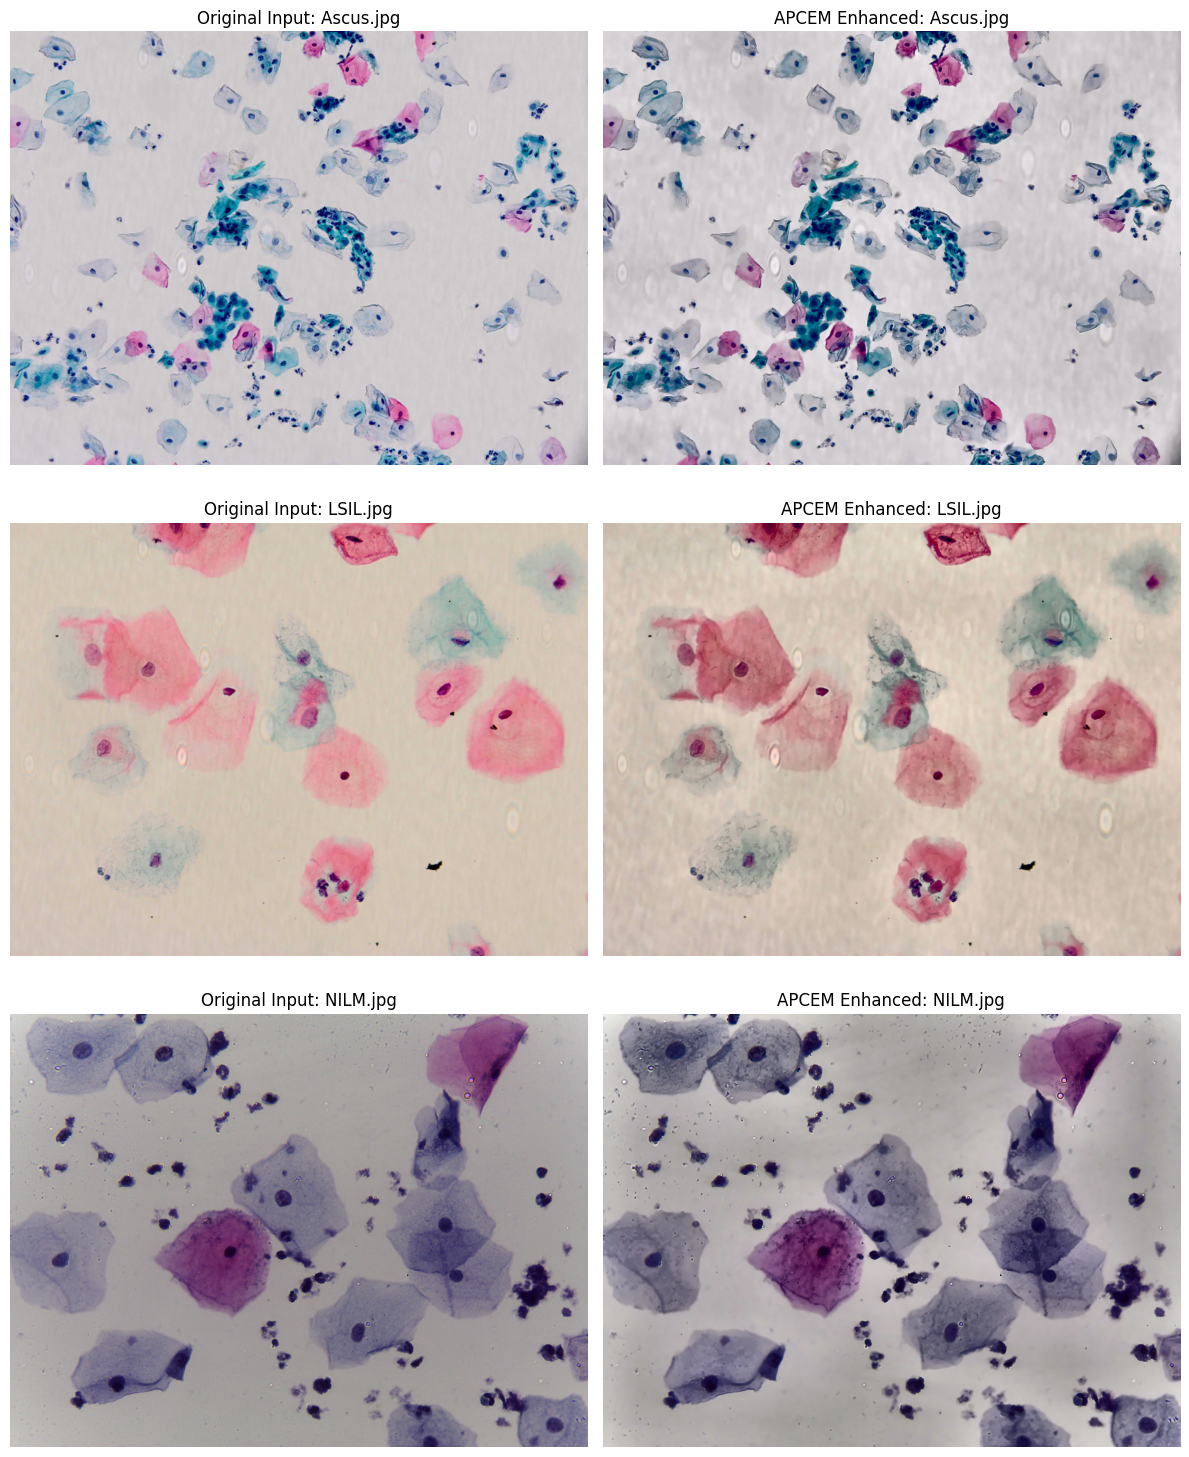
\includegraphics[width=0.8\textwidth]{image/APCEM.png} 
    \caption{Qualitative evaluation of the APCEM model. Left: Original raw input images. Right: Preprocessed outputs}
    \label{apcem}
\end{figure}
    
    \item \textbf{LAB-space contrast enhancement using CLAHE:} To improve the visibility of cytological structures while preserving the original color characteristics of the images, Contrast Limited Adaptive Histogram Equalization(CLAHE) was applied in the CIE LAB color space. At first, raw cytology images $\mathbf{I} \in \mathbb{R}^{H \times W \times 3}$ are converted from RGB to the CIE lab color space. Then the resulting image was decomposed into the lightness ($L$) and chromatic ($a$ and $b$) channels. To enhance local image contrast without amplifying color distortion or background noise, CLAHE was applied exclusively to the $L$ channel using a clip limit of $\tau = 2.0$ and an $8\times8$ tile grid. 
    $$L_{\text{enhanced}} = \text{CLAHE}\left(L, \text{clipLimit}=2.0, \text{gridSize}=(8, 8)\right)$$

  This process minimizes unwanted changes to the original color information while improving local luminance contrast and making subtle cellular and nuclear structures easier to see.

    \item \textbf{Non-Local Means (NLM) filtering:} Following CLAHE-based contrast enhancement, Non-Local Means (NLM) filtering was applied to reduce noise and imaging artifacts while preserving important cellular structures. The \textbf{fastNlMeansDenoisingColored()} method was experimented with different values of \textit{h(Filter strength for luminance)}, $\mathit{h_{\mathrm{color}}}$\textit{(Filter strength for color components)}, a \(7\times7\) template window, and a \(21\times21\) search window. Experiment result is shown in Table~\ref{tab:denoising_parameters}. As $h$\textit{=5} and $h_{\mathrm{color}}$\textit{=5} provide better segmentation mask, we further run the model with these values. 
    
  \begin{table}[ht]
    \centering
     \caption{Effect of different denoising parameters on Dice score.}
    \label{tab:denoising_parameters}
    \begin{tabular}{|c|c|c|}
        \hline
        $h$ & $h_{\mathrm{color}}$ & Dice score \\ \hline
        10 & 10 & 45.14 \\ \hline
        \textbf{5} & \textbf{5} & \textbf{47.44} \\ \hline
        5 & 7 & 46.32 \\ \hline
    \end{tabular}
\end{table}

     This operation suppresses unwanted noise while maintaining relevant structures such as nuclear boundaries and cellular morphology. 
    
    \item \textbf{Controlled sharpening via unsharp masking:} The denoised image was then passed for unsharp masking to enhance nuclear and cytoplasmic boundaries.  A Gaussian blurred representation $\mathbf{I}_{\text{blur}}$ is generated using a $3 \times 3$ kernel with a standard deviation $\sigma = 1.0$:$$\mathbf{I}_{\text{blur}} = \mathbf{I}_{\gamma} * \mathbf{G}_{\sigma=1.0}$$The final enhanced image $\mathbf{I}_{\text{APCEM}}$ is synthesized through weighted high-frequency residual injection:$$\mathbf{I}_{\text{APCEM}} = \text{clip}\left(1.5 \cdot \mathbf{I}_{\gamma} - 0.5 \cdot \mathbf{I}_{\text{blur}}, 0, 1\right)$$
    The resulting intensity values were subsequently clipped to the range $[0,1]$ to maintain a valid normalized image representation.
\end{itemize}

\subsection{Nucleus Mask Extractor}
In the Sipakmed dataset, boundary areas of cytoplasm and the cell nucleus are manually annotated by clinicians. Thus, we can directly perform segmentation on it without extracting mask. But for other two cytology datasets, we have to develope an automated, morphologically guided segmentation pipeline that will extract the nucleus mask. And the reason behind choosing a nucleus mask is that in a cancerous cell characteristics of a nucleus change more than those of a cytoplasm. 

The main goal was to convert the nucleus to white and the background to black. At first, each RGB cytology image was transformed into a grayscale representation and smoothed using a 5×5 Gaussian filter to suppress noise and staining artifacts. \textbf{Adaptive Gaussian thresholding} (block size = 21, constant offset C = 5) was then applied, using binary inversion to highlight comparatively darker nuclear areas as foreground. The resulting binary mask was modified using morphological opening with a 3×3 elliptical structuring element to minimize small isolated artifacts, followed by morphological closing to fill small gaps and holes within the detected regions. The cleaned mask was then used to identify external outlines. In order to create the final binary nucleus mask, which has pixel values of 255 for the foreground nucleus and 0 for the background, the biggest contour was chosen as the supposed nucleus and filled. The morphologically processed binary mask was kept as the output when no contour was found. This process generates pseudo-nucleus masks automatically, which the proposed architecture can employ as segmentation targets.


\subsection{Proposed Model Architecture} We propose a joint multi-task Res-UNet architecture with a self-attention bottleneck mechanism shown in Figure~\ref{architecture} for simultaneous nucleus segmentation and cervical cell classification. The main motivation is to learn a common feature representation that is able to capture both the spatial characteristics of the nucleus and the discriminative morphological features needed for cell-type classification. The model is based on an encoder–decoder architecture, with a multi-head self-attention mechanism at the bottleneck and two task-specific output branches for segmentation and classification.

\begin{figure}[htbp]
    \centering
    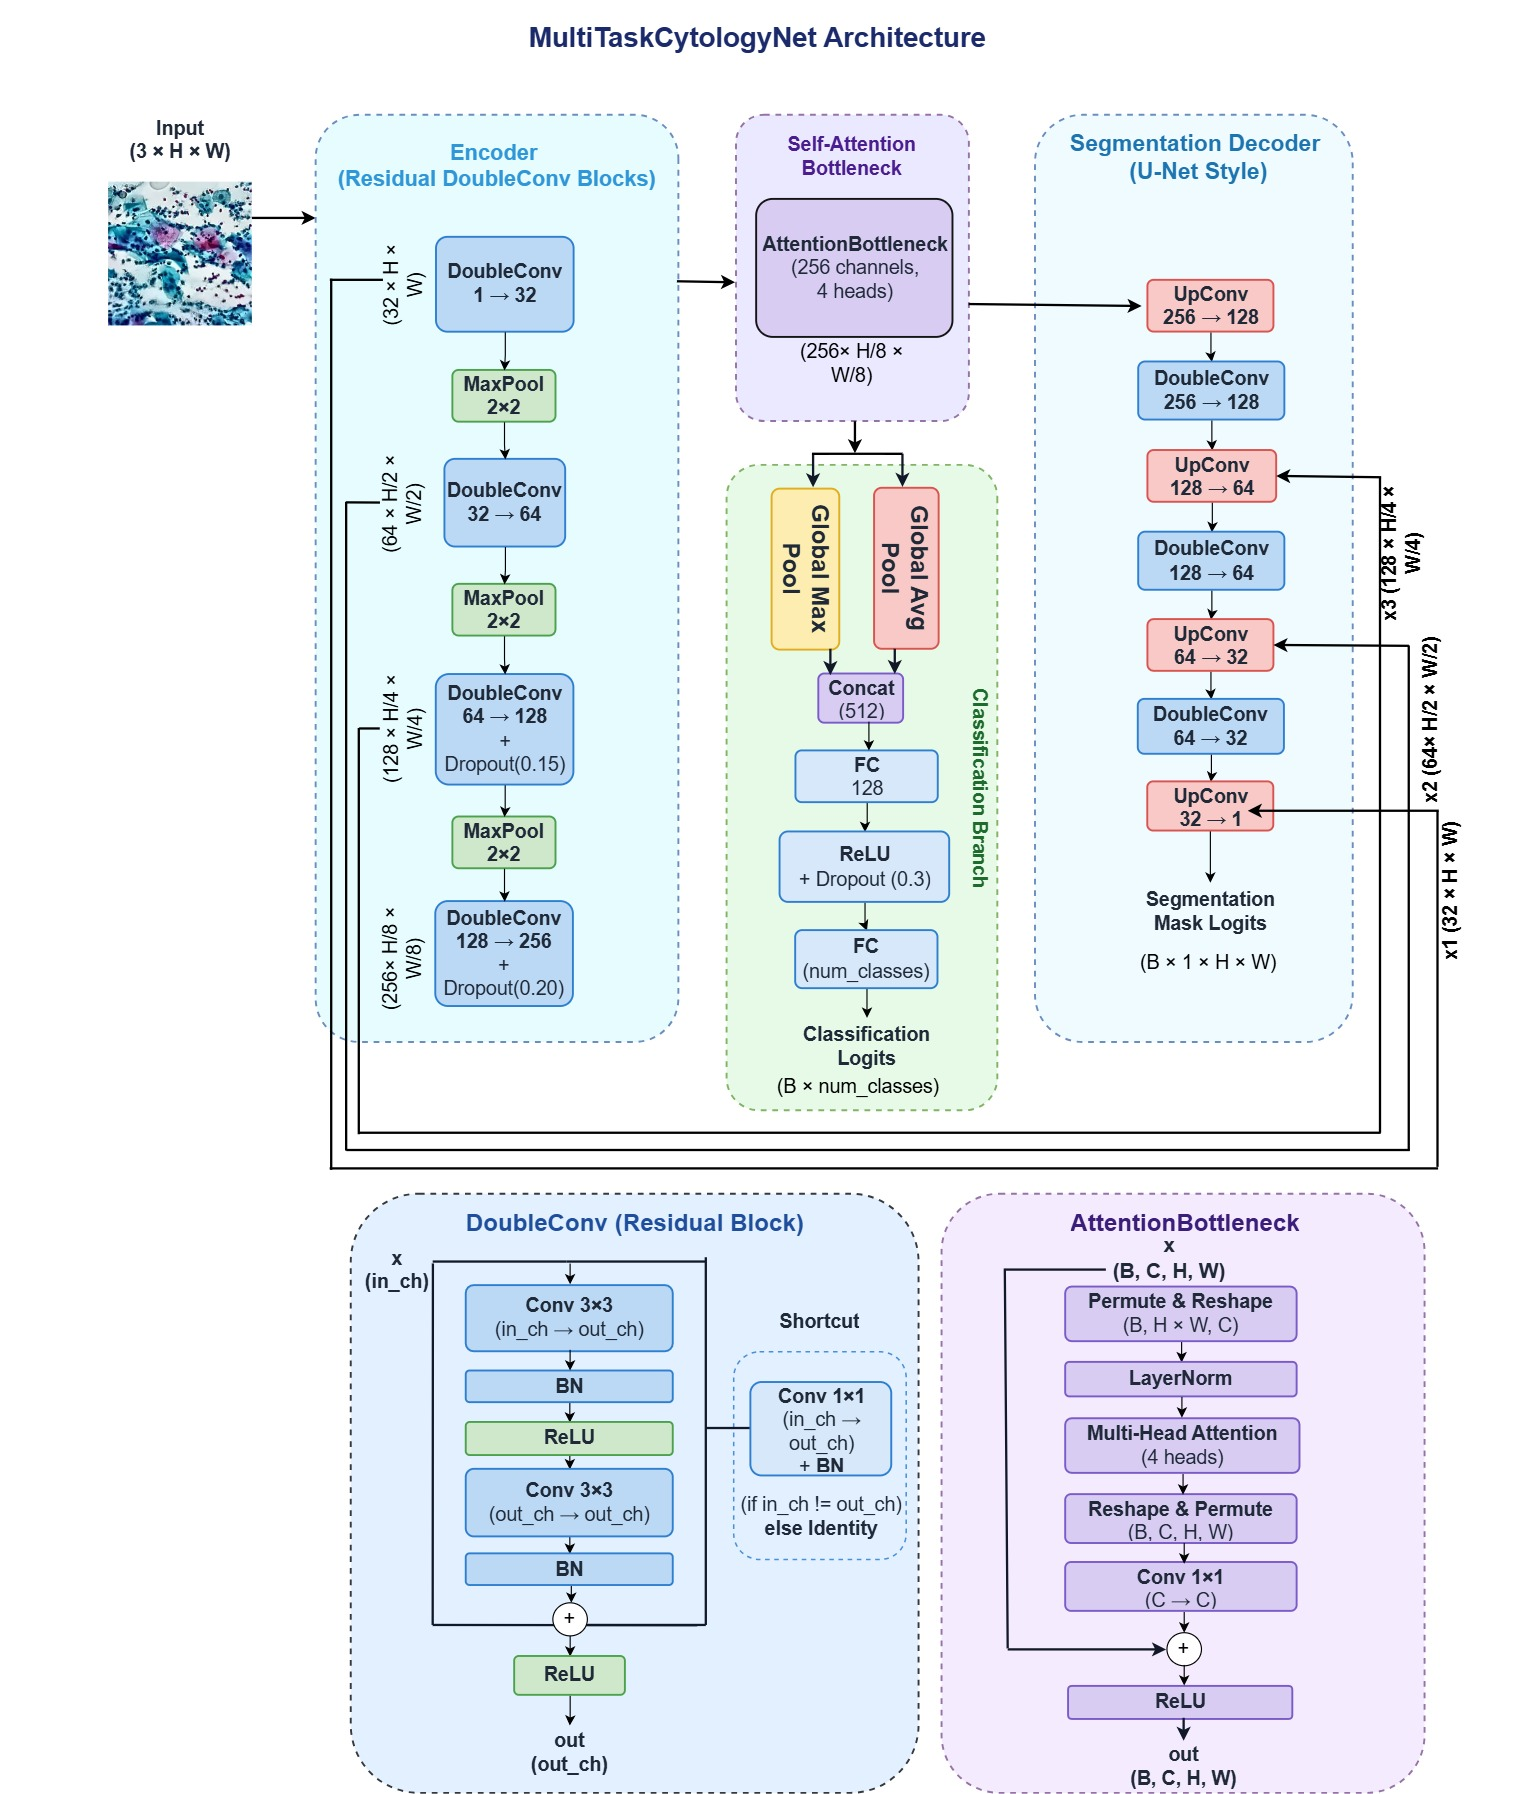
\includegraphics[width=1.1\textwidth]{image/MultiTaskCytologyNet_Architecture1 (5).jpg} 
    \caption{Attention enhanced multi-task Res-UNet architecture}
    \label{architecture}
\end{figure}

\subsubsection{CNN Encoder}
The encoder consists of four residual stages that progressively extract hierarchical visual representations while reducing spatial resolution. The fundamental building block is a residual Double Convolution (\textbf{DoubleConv}) block, comprising two consecutive $3 \times 3$ 2D convolutional layers, each followed by Batch Normalization (BN) and ReLU non-linear activation. To facilitate gradient propagation and feature reuse across scales, a residual shortcut connection $\mathcal{F}_{\text{res}}(x)$ is incorporated:
\begin{equation}
    \text{DoubleConv}(x) = \text{ReLU}\Big(\text{BN}\big(\text{Conv}_{3\times3}(\text{ReLU}(\text{BN}(\text{Conv}_{3\times3}(x))))\big) + \mathcal{F}_{\text{res}}(x)\Big)
\end{equation}
where $\mathcal{F}_{\text{res}}(x) = \text{BN}(\text{Conv}_{1\times1}(x))$ when the input and output channel dimensions differ, and the identity mapping $\mathcal{F}_{\text{res}}(x) = x$ otherwise.

Spatial downsampling is achieved using $2 \times 2$ Max Pooling operations between stages. Spatial Dropout with rates of 0.15 and 0.20 is incorporated after the third and fourth encoder stages, respectively, to mitigate overfitting. Given an RGB input image of size $3 \times 224 \times 224$, the encoder produces a bottleneck feature representation of dimension $256 \times 28 \times 28$.

\subsubsection{Multi-Head Self-Attention Bottleneck}
Standard convolutional operation cannot capture the relationship between distant pixels of an image which is important for distinguishing inter-class differences. Thus, we integrate multi-head self-attention at the bottleneck to capture non-local, long-range contextual relationships across distant regions of an image. Attention is applied on the deepest feature map (256×28×28), which is converted into sequence of spatial tokens (256x784). Layer normalization is then applied, followed by multi-head self-attention(MHSA) with four attention heads on these tokens. And then reshaped back to its original spatial form (256×28×28) and fused with the original feature map via a residual 1×1 convolutional projection:

$$\hat{x} = \mathrm{ReLU}\big(x + \mathrm{Conv}_{1\times1}(\mathrm{MHSA}(\mathrm{LN}(x)))\big)$$

Now, $\hat{x}$ contain local convolutional features as well as global contextual information. 

\subsubsection{Dual-Task Output Head}
Our proposed model does two task at once—cancer cell classification and nucleus mask segmentation. Thus it has two output branches-- 

\begin{itemize}

\item{\textbf{Classification Head:}} The bottleneck feature map (256×28×28) is now converted to 256-dimensional feature vector using both global average pooling (GAP) and global max pooling (GMP), and the two pooled 256-dimensional vectors are concatenated to form 512 dimensional representation. GAP captures the general distribution of learned features, whereas GMP emphasizes the strongest feature responses. When combined, they offer complimentary global and significant feature information for classification. The concatenated vector is passed through a fully connected layer (512 → 128) with ReLU activation and dropout (0.3), followed by a final fully connected layer (128 → 5) producing classification logits for the five cervical cell categories.

\item{\textbf{Segmentation Head:}}
Along with classification, the attention-enhanced bottleneck features are passed to a U-Net-inspired decoder in parallel for nucleus segmentation. The decoder progressively restores the  bottleneck features back to the input resolution. At each decoder stage, transposed convolution layer is used for upsampling, followed by concatenation with the corresponding encoder feature map through skip connections. Skip connections concatenate the high resolution feature maps from the encoder stages (x1, x2, x3) directly to their corresponding decoder stages (up1, up2, up3) in to restore the spatial detail lost during downsampling. The concatenated representations are then processed through \textbf{DoubleConv} blocks to enhance localized features, ending with a $1 \times 1$ convolution layer to produce a single-channel segmentation logit map representing the predicted nucleus region.
\end{itemize}


\subsubsection{Network Parameter Distribution and Model Complexity}
To evaluate the computational efficiency and deployability of the proposed multi-task architecture, we conducted a structural layer-wise parameter audit. The network contains a total of $2,410,310$ trainable parameters ($\approx 2.41$\,M), consuming approximately $8.19$\,MB of parameter memory. The layer-wise breakdown across the four primary sub-modules is summarized in Table~\ref{tab:param_distribution}.

\begin{table}[htbp]
\centering
\caption{Parameter Distribution Across Sub-Modules in the Proposed Multi-Task Network}
\label{tab:param_distribution}
\begin{tabular}{lrr}
\hline
\textbf{Sub-Module} & \textbf{Parameter Count} & \textbf{Percentage (\%)} \\
\hline
CNN Encoder (Backbone)          & 1,217,280 & 50.50\% \\
Multi-Head Attention Bottleneck &   329,472 & 13.67\% \\
Segmentation Decoder Branch     &   797,249 & 33.08\% \\
Dual-Pooling Classification Head&    66,309 &  2.75\% \\
\hline
\textbf{Total Trainable Parameters} & \textbf{2,410,310} & \textbf{100.00\%} \\
\hline
\end{tabular}
\end{table}

As detailed in Table~\ref{tab:param_distribution}, over half of the network's capacity ($50.50\%$) is concentrated in the shared feature encoder, ensuring robust multi-scale hierarchical feature extraction. The four-stage transposed convolution segmentation decoder constitutes $33.08\%$ of the parameters, providing the spatial reconstruction capacity needed to delineate delicate nuclear borders. The Multi-Head Self-Attention (MHSA) bottleneck requires only $329,472$ parameters ($13.67\%$) while equipping the latent space with global receptive field capabilities. Finally, the classification head is exceptionally lightweight, comprising only $66,309$ parameters ($2.75\%$). This compact footprint prevents classifier overfitting while extracting global contextual representations via concatenated average and maximum pooling.


\subsubsection{Composite Multi-Task Loss Formulation}
The multi-task network is trained end-to-end using a joint objective function that combines classification and boundary segmentation penalties:
\begin{equation}
    \mathcal{L}_{\text{total}} = \mathcal{L}_{\text{seg}} + \lambda \mathcal{L}_{\text{cls}}
\end{equation}
where $\lambda = 1.0$. The classification loss $\mathcal{L}_{\text{cls}}$ is standard categorical Cross-Entropy:
\begin{equation}
    \mathcal{L}_{\text{cls}} = - \sum_{c=1}^{C} y_c \log(\hat{y}_c)
\end{equation}
where $y_c$ and $\hat{y}_c$ denote the ground-truth binary indicator and predicted class probability for class $c$, respectively. 

The segmentation objective $\mathcal{L}_{\text{seg}}$ combines pixel-wise Binary Cross-Entropy with soft Dice loss to handle class imbalance between nuclear and non-nuclear background pixels:
\begin{equation}
    \mathcal{L}_{\text{seg}} = \mathcal{L}_{\text{BCE}}(M, \hat{M}) + \mathcal{L}_{\text{Dice}}(M, \hat{M})
\end{equation}
\begin{equation}
    \mathcal{L}_{\text{Dice}}(M, \hat{M}) = 1 - \frac{2 \sum_{i=1}^{H \times W} \sigma(\hat{M}_i) M_i + \epsilon}{\sum_{i=1}^{H \times W} \sigma(\hat{M}_i) + \sum_{i=1}^{H \times W} M_i + \epsilon}
\end{equation}
where $\sigma(\cdot)$ is the sigmoid function, $M_i \in \{0, 1\}$ is the target pixel mask, $\hat{M}_i$ is the raw predicted segmentation logit, and $\epsilon = 1.0$ is a Laplacian smoothing parameter.

\subsubsection{Training Strategy and Hyperparameters}
Models were implemented in PyTorch and trained for 50 epochs using an NVIDIA GPU. We employed the AdamW optimizer with an initial learning rate $\eta = 1 \times 10^{-3}$ and weight decay of $1 \times 10^{-4}$. A dynamic \texttt{ReduceLROnPlateau} scheduler monitored validation loss, reducing the learning rate by a factor of 0.2 with a patience of 5 epochs. A mini-batch size of 16 was used across all experiments. The model checkpoint exhibiting minimum total validation loss was selected for final test set evaluation.


\subsection{Evaluation Metrics}
The predictive performance of the classification model was evaluated using five common metrics. These are the confusion matrix, accuracy, precision, recall, and F1 score. Together, they give an objective and quantitative measure of how well each model predicts.

The confusion matrix compares the predicted class with the actual class for each case. For a binary problem, it has four entries. True positives (TP) are positive cases that the model correctly identifies. True negatives (TN) are the total number of correctly recognized negative instances. False positives (FP) are negative cases that the model wrongly labels as positive. False negatives (FN) are the count of positive instances misclassified as negative. All other metrics are calculated from these four values. They are mathematically defined as follows:

\begin{equation}
    \text{Accuracy} = \frac{TP + TN}{TP + TN + FP + FN}
    \label{eq:accuracy}
\end{equation}

\begin{equation}
    \text{Precision} = \frac{TP}{TP + FP}
    \label{eq:precision}
\end{equation}

\begin{equation}
    \text{Recall} = \frac{TP}{TP + FN}
    \label{eq:recall}
\end{equation}

\begin{equation}
    \text{F1 score} = \frac{2 \times \text{Precision} \times \text{Recall}}{\text{Precision} + \text{Recall}}
    \label{eq:f1}
\end{equation}

The overall correctness of the model across all predictions is defined by accuracy. Precision shows how many of the individuals predicted to have cervical cancer actually have it. Recall evaluates the ability of the model to find all individuals who actually have cervical cancer. The harmonic mean of precision and recall is determined by F1 score.


The Dice score was used to evaluate segmentation performance. It measures the overlap between the region predicted by the model and the ground truth masks. It is defined as:


\begin{equation}
    \text{Dice score} = \frac{2\,|X \cap Y|}{|X| + |Y|} = \frac{2\,TP}{FP + 2\,TP + FN}
    \label{eq:dice}
\end{equation}

\noindent where $X$ is the predicted region and $Y$ is the ground truth region.

\section{Result Analysis}\label{sec4}

We have divided this section as three parts—Multiclass classification, Binary class classification, and Segmentation.

\subsection{Multiclass classification}
\subsubsection{SipakMed}
Our proposed model was trained for 50 epochs on the Sipakmed dataset. It showed overall high performance across five classes by achieving test accuracy of 96.38\%. Figure \ref{sipakMulti} shows the training and validation curve of loss and accuracy. Both the curves remain closely aligned throughout training with no divergence in later epochs, indicating that the model did not suffer from significant overfitting despite multitasking.

\begin{figure}[htbp]
    \centering
    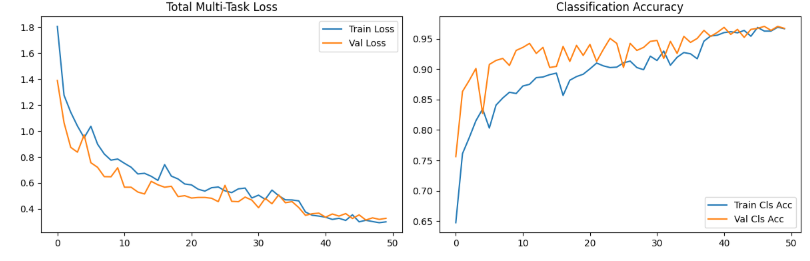
\includegraphics[width=0.8\textwidth]{image/multi/sipakMulti.png} 
    \caption{Loss \& Accuracy Curve of Sipakmed Dataset}
    \label{sipakMulti}
\end{figure}

Table \ref{tab:classification_report_sipak} represents the overall classification report for 5 classes. Among all the classes the proposed multi-task model achieved the highest precision, recall and F1-score of 0.99 for the Parabasal class. Whereas, the koilocytotic cell recorded the lowest performance comparatively (precision = 0.93, recall = 0.91, F1 = 0.92), because of the morphological overlap between koilocytotic and dyskeratotic cells in cervical cytology. The macro-averaged and weighted-averaged precision, recall, and F1-scores both converged to 0.96. These findings show that the model's classification ability is comparatively constant across the five cytological classes.

\begin{table}[htbp]
    \centering
    \caption{Classification Report of Sipakmed Dataset}
    \label{tab:classification_report_sipak}
    \begin{tabular}{lcccc}
        \toprule
        \textbf{Class} & \textbf{Precision} & \textbf{Recall} & \textbf{F1-Score} & \textbf{Support} \\
        \midrule
        Dyskeratotic             & 0.97 & 0.97 & 0.97 & 122 \\
        Koilocytotic             & 0.93 & 0.91 & 0.92 & 124 \\
        Metaplastic              & 0.97 & 0.96 & 0.97 & 119 \\
        Parabasal                & 0.99 & 0.99 & 0.99 & 118 \\
        Superficial Intermediate & 0.95 & 0.99 & 0.97 & 125 \\
        \bottomrule
    \end{tabular}
\end{table}

\subsubsection{APCEM-Enhanced Cervical Cytology Image Dataset}

To the best of our knowledge, this study provides the first benchmark evaluation of a deep learning framework on this recently published dataset, establishing baseline findings for both cervical cell classification and nucleus segmentation. During the training, there is an overall decreasing and increasing trend in loss and accuracy, respectively, without too many fluctuations shown in Figure \ref{cytologyData1}. The model achieved an overall test accuracy of 76.65\%. Macro-averaged precision, recall, and F1-score are 0.74, whereas the weighted average score is about 0.76. 

\begin{figure}[htbp]
    \centering
    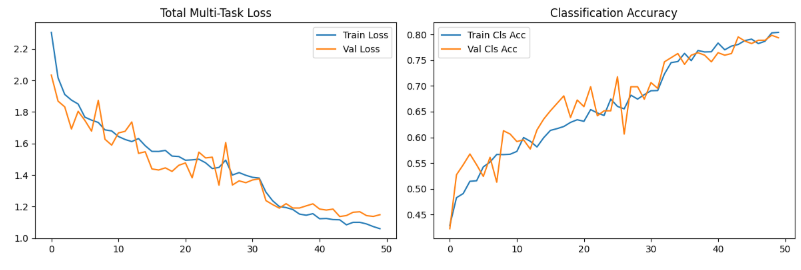
\includegraphics[width=0.8\textwidth]{image/multi/cytology_data1.png} 
    \caption{Loss \& Accuracy Curve of APCEM-Enhanced Cervical Cytology Dataset}
    \label{cytologyData1}
\end{figure}

This dataset is an imbalanced dataset due to which model tends to perform biasedly. ASCUS class has the lowest test sample(51) leading to lowest performance with a recall of only 0.33 and an F1-score of 0.40, indicating that the majority of true ASCUS samples were misclassified into other categories. HSIL, LSIL, and SCC achieve F1-scores of 0.72, 0.74, and 0.85, respectively. The highest F1-score was achieved by the NILM class. Overall classification performance for this dataset is shown in Table \ref{tab:classification_report_cyt1}.

\begin{table}[htbp]
    \centering
    \caption{Classification Report of APCEM-Enhanced Cervical Cytology Image Dataset}
    \label{tab:classification_report_cyt1}
    \begin{tabular}{lcccc}
        \toprule
        \textbf{Class} & \textbf{Precision} & \textbf{Recall} & \textbf{F1-Score} & \textbf{Support} \\
        \midrule
        ASCUS & 0.52 & 0.33 & 0.40 & 51 \\
        HSIL  & 0.76 & 0.69 & 0.72 & 195 \\
        LSIL  & 0.69 & 0.79 & 0.74 & 187 \\
        NILM  & 0.98 & 0.96 & 0.97 & 117 \\
        SCC   & 0.78 & 0.93 & 0.85 & 71 \\
        \bottomrule
    \end{tabular}
\end{table}

\subsubsection{CytologCervicalCancer}

The proposed multi-task model was further evaluated on the \textbf{CytologCervicalCancer} dataset to assess the generalizability of the architecture across a third distinct data distribution. This dataset is categorized into the same five diagnostic classes as the APCEM-enhanced dataset. To ensure a direct and standardized evaluation process across the two datasets, we implemented the APCEM preprocessing model on CytologCervicalCancer dataset. Though the number of sample in each class is less than dataset \cite{aswini2026apcem}, the model trained better on this dataset.

\begin{figure}[htbp]
    \centering
    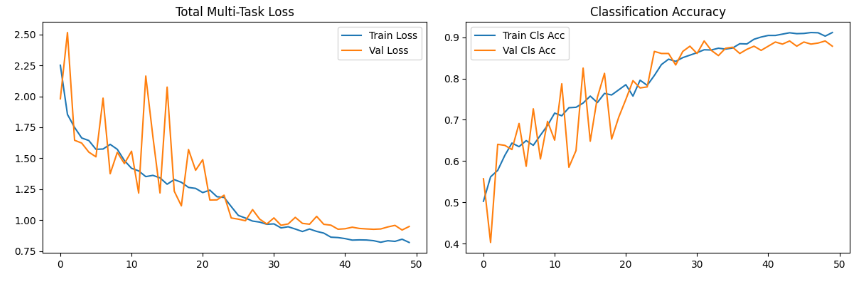
\includegraphics[width=0.8\textwidth]{image/multi/cytology_data2.png} 
    \caption{Loss \& Accuracy Curve of CytologCervicalCancer}
    \label{cytologyData2}
\end{figure}

The model had unstable optimization dynamics and validation loss fluctuated a lot during the first 20 epochs, perhaps because the per-class sample sizes were quite small and imbalanced (from only 30 to 127 photos), but it eventually converged to a stable level after 40 epochs without significant overfitting, as shown in Figure~\ref{cytologyData2}. Overall, the model achieved a higher accuracy of 88.64\% on test set.

Table~\ref{tab:classification_report_Cyt2} shows the precision, recall and F1-score of each class. ASCUS class has the lowest sample in both the datasets. Still, the model achieved a fairly strong F1-score of 0.79 (precision = 0.82, recall = 0.77)—a considerable improvement from the severe ASCUS misclassification on the APCEM-enhanced dataset, which suggests that ASCUS instances in this dataset are morphologically more distinct or less affected by preprocessing-induced noise. It classified NILM class with 100\% F1-score, while LSIL and SCC both achieved F1-scores of 0.87, and HSIL achieved an F1-score of 0.85. Overall, the model shows strong and fairly balanced performance for this dataset.

\begin{table}[htbp]
    \centering
    \caption{Classification Report of CytologCervicalCancer Dataset}
    \label{tab:classification_report_Cyt2}
    \begin{tabular}{lcccc}
        \toprule
        \textbf{Class} & \textbf{Precision} & \textbf{Recall} & \textbf{F1-Score} & \textbf{Support} \\
        \midrule
        ASCUS & 0.82 & 0.77 & 0.79 & 30 \\
        HSIL  & 0.82 & 0.87 & 0.85 & 127 \\
        LSIL  & 0.89 & 0.85 & 0.87 & 92 \\
        NILM  & 1.00 & 1.00 & 1.00 & 92 \\
        SCC   & 0.89 & 0.85 & 0.87 & 55 \\
        \bottomrule
    \end{tabular}
\end{table}

\subsubsection{Merged Custom Cervical Cytology Dataset}

To increase the overall size and diversity of the training data, the APCEM-enhanced and Cytology Cervical Cancer datasets were merged into a single combined corpus. And the model achieved higher accuracy of 88.98\% for the custom dataset than individual ones. The loss curve follows the almost same decreasing pattern as the individual datasets. But the accuracy curve shows a steady, comparatively smoother climb than either individual dataset shown in Figure~\ref{customCutology}  

\begin{figure}[htbp]
    \centering
    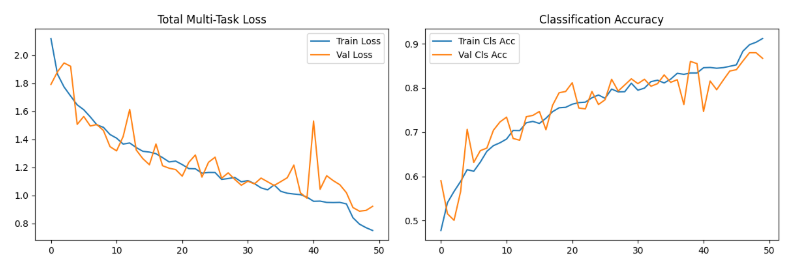
\includegraphics[width=0.8\textwidth]{image/multi/merge.png} 
    \caption{Loss \& Accuracy Curve of CytologCervicalCancer}
    \label{customCutology}
\end{figure}

The per-class classification report in Table~\ref{tab:classification_report_cutom} certifies that the proposed model performed better for HSIL(F1-score=0.87), LSIL(F1-score=0.87), NILM(F1-score=0.98), and SCC(F1-score=0.94) class. The lowest performing ASCUS class achieved a higher precision(0.83) in this case, but lower F1-score of 0.72 compared to CytologCervicalCancer(F1=0.79) and improvement over the APCEM enhanced dataset(F1 = 0.40).

\begin{table}[htbp]
    \centering
    \caption{Classification Report of Custom Cervical Cytology Dataset}
    \label{tab:classification_report_cutom}
    \begin{tabular}{lcccc}
        \toprule
        \textbf{Class} & \textbf{Precision} & \textbf{Recall} & \textbf{F1-Score} & \textbf{Support} \\
        \midrule
        ASCUS & 0.83 & 0.64 & 0.72 & 81 \\
        HSIL  & 0.88 & 0.86 & 0.87 & 322 \\
        LSIL  & 0.83 & 0.91 & 0.87 & 278 \\
        NILM  & 0.99 & 0.96 & 0.98 & 209 \\
        SCC   & 0.92 & 0.96 & 0.94 & 126 \\
        \bottomrule
    \end{tabular}
\end{table}


\subsection{Binary Classification}

For binary classification(Normal and Abnormal), the model was trained on Sipakmed\cite{Lite38} and custom cytology dataset. And it performed exceptionally well for both the datasets.

\subsubsection{Sipakmed}
The proposed architecture achieves a higher test accuracy of 97.86\% and class-wise accuracy is also very high. The loss and accuracy curve is shown in Figure~\ref{binarySipak}. Training and validation curves are relatively close but converge to a stable level with a limited generalization gap.

\begin{figure}[htbp]
    \centering
    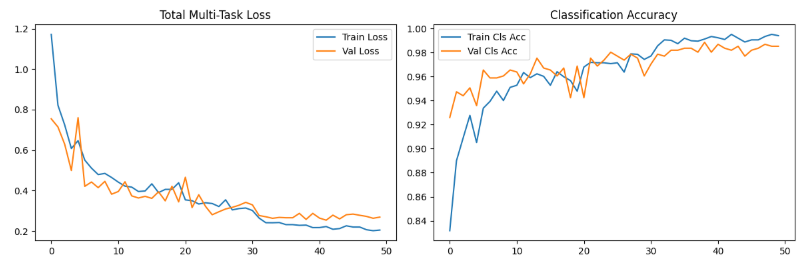
\includegraphics[width=0.8\textwidth]{image/binary/sipakmed.png} 
    \caption{Loss \& Accuracy Curve of Sipakmed for binary classification}
    \label{binarySipak}
\end{figure}

Class-wise performance is also very high (Table~\ref{tab:classification_report_binary}). The normal class achieved a 0.97 F1-Score, while the Abnormal class achieved 0.98 F1-Score which is pretty high. In addition to classification, the jointly trained segmentation branch achieves a mean nucleus Dice score of 0.8801.

\begin{table}[htbp]
    \centering
    \caption{Classification Report of Sipakmed dataset for Binary Classification}
    \label{tab:classification_report_binary}
    \begin{tabular}{lcccc}
        \toprule
        \textbf{Class} & \textbf{Precision} & \textbf{Recall} & \textbf{F1-Score} & \textbf{Support} \\
        \midrule
        Normal   & 0.98 & 0.97 & 0.97 & 243 \\
        Abnormal & 0.98 & 0.98 & 0.98 & 365 \\
        \bottomrule
    \end{tabular}
\end{table}

\subsubsection{Custom Cervical Cytology Dataset}
We constructed the custom dataset for binary classification also, and it's a balanced dataset. On the test dataset the model achieved an higher accuracy of 98.56\%, but a very low Dice Score (0.4230) for nucleus segmentation. Both the loss and accuracy curves became stable after 25 epochs and remained in a steady state till 50 epochs (figure \ref{binaryCustom}). 

\begin{figure}[htbp]
    \centering
    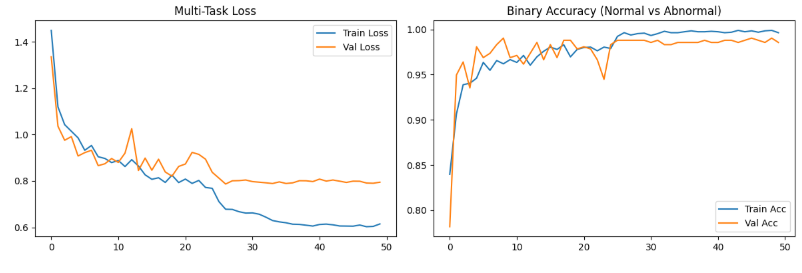
\includegraphics[width=0.8\textwidth]{image/binary/custom.png} 
    \caption{Loss \& Accuracy Curve of Custom Dataset for Binary classification}
    \label{binaryCustom}
\end{figure}

The model classified both the classes with high precision and very few false predictions. Classification report in Table~\ref{tab:classification_report_binary2} indicates very strong and balanced performance for both classes. Normal class achieved a perfect score in precision, whereas abnormal class achieved a perfect score in recall.

\begin{table}[htbp]
    \centering
    \caption{Classification Report of Custom Dataset for Binary Classification}
    \label{tab:classification_report_binary2}
    \begin{tabular}{lcccc}
        \toprule
        \textbf{Class} & \textbf{Precision} & \textbf{Recall} & \textbf{F1-Score} & \textbf{Support} \\
        \midrule
        Normal   & 1.00 & 0.98 & 0.99 & 209 \\
        Abnormal & 0.98 & 1.00 & 0.99 & 209 \\
        \bottomrule
    \end{tabular}
\end{table}

\subsection{Segmentation}
The training and validation nucleus segmentation Dice scores of the proposed multi-task framework across four cervical cytology datasets is presented in Figure~\ref{fig:main_four_figures}. The curve follows almost the similar trend for the cytology datasets but shows better performance for Sipakmed dataset. On SIPaKMeD, the model achieves a mean test Dice score of 86.46\%, with both training and validation Dice scores showing a steady upward trend and converging near the final epochs. Ground truth annotations of cell nuclues for each image was given in the Sipakmed\cite{Lite38} dataset, because of which model could predict the mask with higher score. 

\begin{figure}[htbp]
    \centering
    % First Row
    \begin{subfigure}[b]{0.48\textwidth}
        \centering
        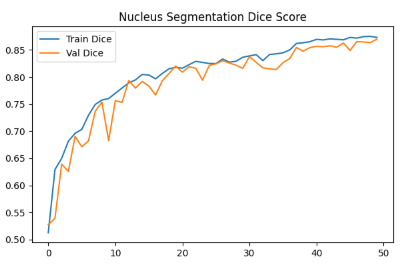
\includegraphics[width=\textwidth]{image/segmentation/sipakmed.png} % Replace with your first image
        \caption{SipakMed}
        \label{fig:sub1}
    \end{subfigure}
    \hfill
    \begin{subfigure}[b]{0.48\textwidth}
        \centering
        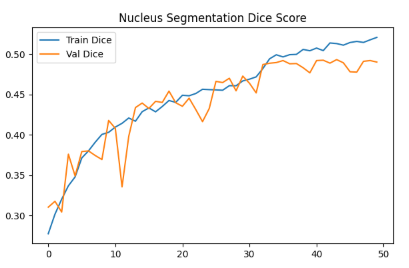
\includegraphics[width=\textwidth]{image/segmentation/cytology1.png} % Replace with your second image
        \caption{APCEM-Enhanced Cervical Cytology}
        \label{fig:sub2}
    \end{subfigure}

    \vspace{0.5cm} % Vertical space between rows

    % Second Row
    \begin{subfigure}[b]{0.48\textwidth}
        \centering
        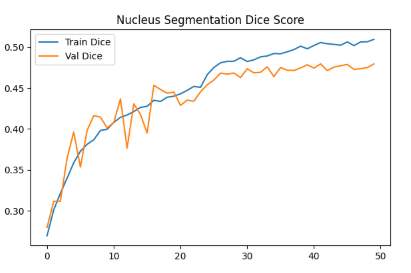
\includegraphics[width=\textwidth]{image/segmentation/cytology2.png} % Replace with your third image
        \caption{CytologCervicalCancer}
        \label{fig:sub3}
    \end{subfigure}
    \hfill
    \begin{subfigure}[b]{0.48\textwidth}
        \centering
        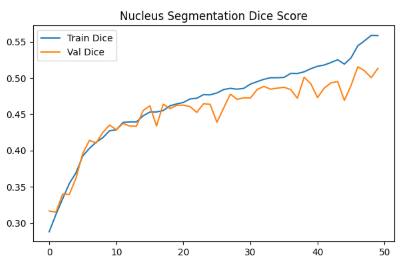
\includegraphics[width=\textwidth]{image/segmentation/custom.png} % Replace with your fourth image
        \caption{Custom Dataset}
        \label{fig:sub4}
    \end{subfigure}

    \caption{Nucleus Segmentation Dice Score}
    \label{fig:main_four_figures}
\end{figure}

In contrast, the model achieves lower test Dice scores of 45.19\% and 49.17\% on the APCEM-Enhanced Cervical Cytology and CytologCervicalCancer datasets, respectively. Although the training and validation curves on these datasets demonstrate continuous improvement, lower score indicates greater difficulty in accurately outlining nuclear boundaries due to image variability and morphological complexity. The Custom Dataset achieves a mean test Dice score of 49.98\%, representing a slight improvement over the individual component datasets. This result suggests that increasing the diversity and scale of the training data can provide some benefit for general nucleus segmentation, although the improvement is modest. These findings also establish dataset-specific benchmark results for nucleus segmentation and provide a reference for future methods evaluated on these datasets.

\subsubsection{Segmentation Results and Qualitative Evaluation}
\label{sec:segmentation_results}

Nuclear morphology—manifesting as nuclear enlargement, coarse hyperchromasia, irregular membrane contours, and an elevated nuclear-to-cytoplasmic (N/C) ratio—serves as the primary cytopathological hallmark of cervical dysplastic progression. Consequently, accurate nuclear localization is vital not only as an interpretable structural biomarker, but also as an internal spatial regularizer that guides cell-type classification.

\subsubsection{Quantitative Segmentation Performance}
The quantitative nucleus segmentation performance of the proposed joint multi-task architecture across all four cohorts is summarized in Table~\ref{tab:segmentation_summary}. Training and validation convergence curves tracking the evolution of the Dice coefficient over 50 epochs are presented in Figure~\ref{fig:main_four_figures}.

\begin{table}[htbp]
    \centering
    \small
    \caption{Nucleus Segmentation Performance Across Experimental Benchmarks}
    \label{tab:segmentation_summary}
    % \usepackage{tabularx} and \usepackage{booktabs} are required in your preamble
    \begin{tabularx}{\textwidth}{@{} X L c c @{}}
        \toprule
        \textbf{Dataset Cohort} & \textbf{Ground-Truth Protocol} & \textbf{Mean Test} & \textbf{IoU / Jaccard} \\
                                &                                & \textbf{Dice (\%)}  & \textbf{(\%)}\textsuperscript{*} \\
        \midrule
        SIPaKMeD & Pathologist Manual Contours & \textbf{86.46} & \textbf{76.15} \\
        \addlinespace[0.6em]
        Cytology Dataset 1 (APCEM-Enhanced) & Automated Pseudo-Masks & 45.19 & 29.19 \\
        \addlinespace[0.6em]
        Cytology Dataset 2 & Automated Pseudo-Masks & 49.17 & 32.60 \\
        \addlinespace[0.6em]
        Merged Custom Cytology Dataset & Automated Pseudo-Masks & \textbf{54.44} & \textbf{37.40} \\
        \bottomrule
    \end{tabularx}
    
    \vspace{0.5ex}
    \begin{flushleft}
        \footnotesize
        \textsuperscript{*}Intersection-over-Union (IoU) derived via the monotonic relationship $\text{IoU} = \text{Dice} / (2 - \text{Dice})$.
    \end{flushleft}
\end{table}


As documented in Table~\ref{tab:segmentation_summary}, the highest segmentation fidelity was achieved on the SIPaKMeD benchmark, obtaining a mean test Dice score of \textbf{86.46\%} ($\approx$76.15\% IoU). As illustrated in Figure~\ref{fig:main_four_figures}(a), both the training and validation Dice curves for SIPaKMeD demonstrated a smooth, steady upward trajectory, converging stably from approximately 51.3\% in early epochs to 87.0\% at Epoch 50 without evidence of boundary divergence or over-regularization.

Conversely, on the cytology cohorts where manual pixel-level delineations were absent, the model achieved test Dice scores of 45.19\% on Cytology Dataset 1, 49.17\% on Cytology Dataset 2, and \textbf{54.44\%} on the Merged Custom Dataset (Figure~\ref{fig:main_four_figures}(b--d)). Crucially, uniting both cytology sources into the Merged Custom Dataset resulted in a substantial \textbf{+9.25\%} and \textbf{+5.27\%} absolute increase in test Dice score over Dataset 1 and Dataset 2 individually. This quantitative leap demonstrates that training across heterogeneous multi-center acquisitions prevents the spatial decoder from fitting to scanner-specific staining artifacts, thereby reinforcing generalized nuclear boundary representations.

\begin{figure*}[htbp]
    \centering
    % Row 1
    \begin{subfigure}[b]{0.49\textwidth}
        \centering
        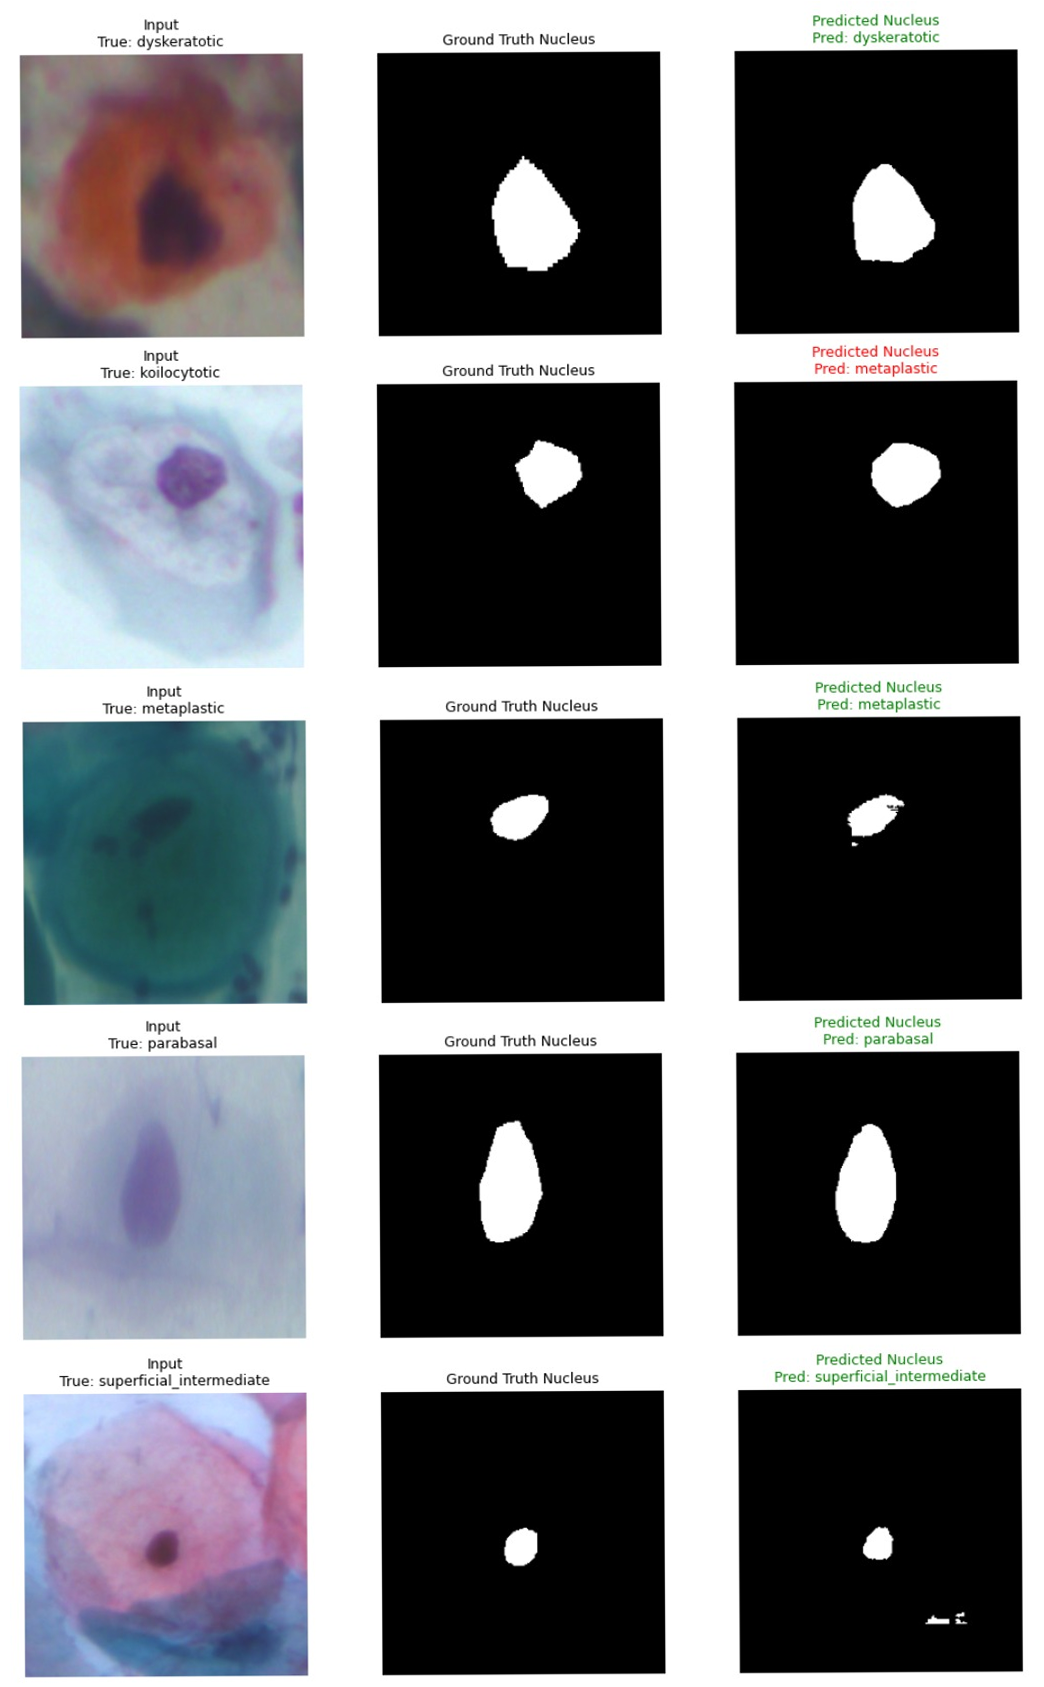
\includegraphics[width=\textwidth]{image/segmentation/sipakGroup 1.png}
        \caption{SIPaKMeD}
        \label{fig:qual_sipak}
    \end{subfigure}
    \hfill
    \begin{subfigure}[b]{0.49\textwidth}
        \centering
        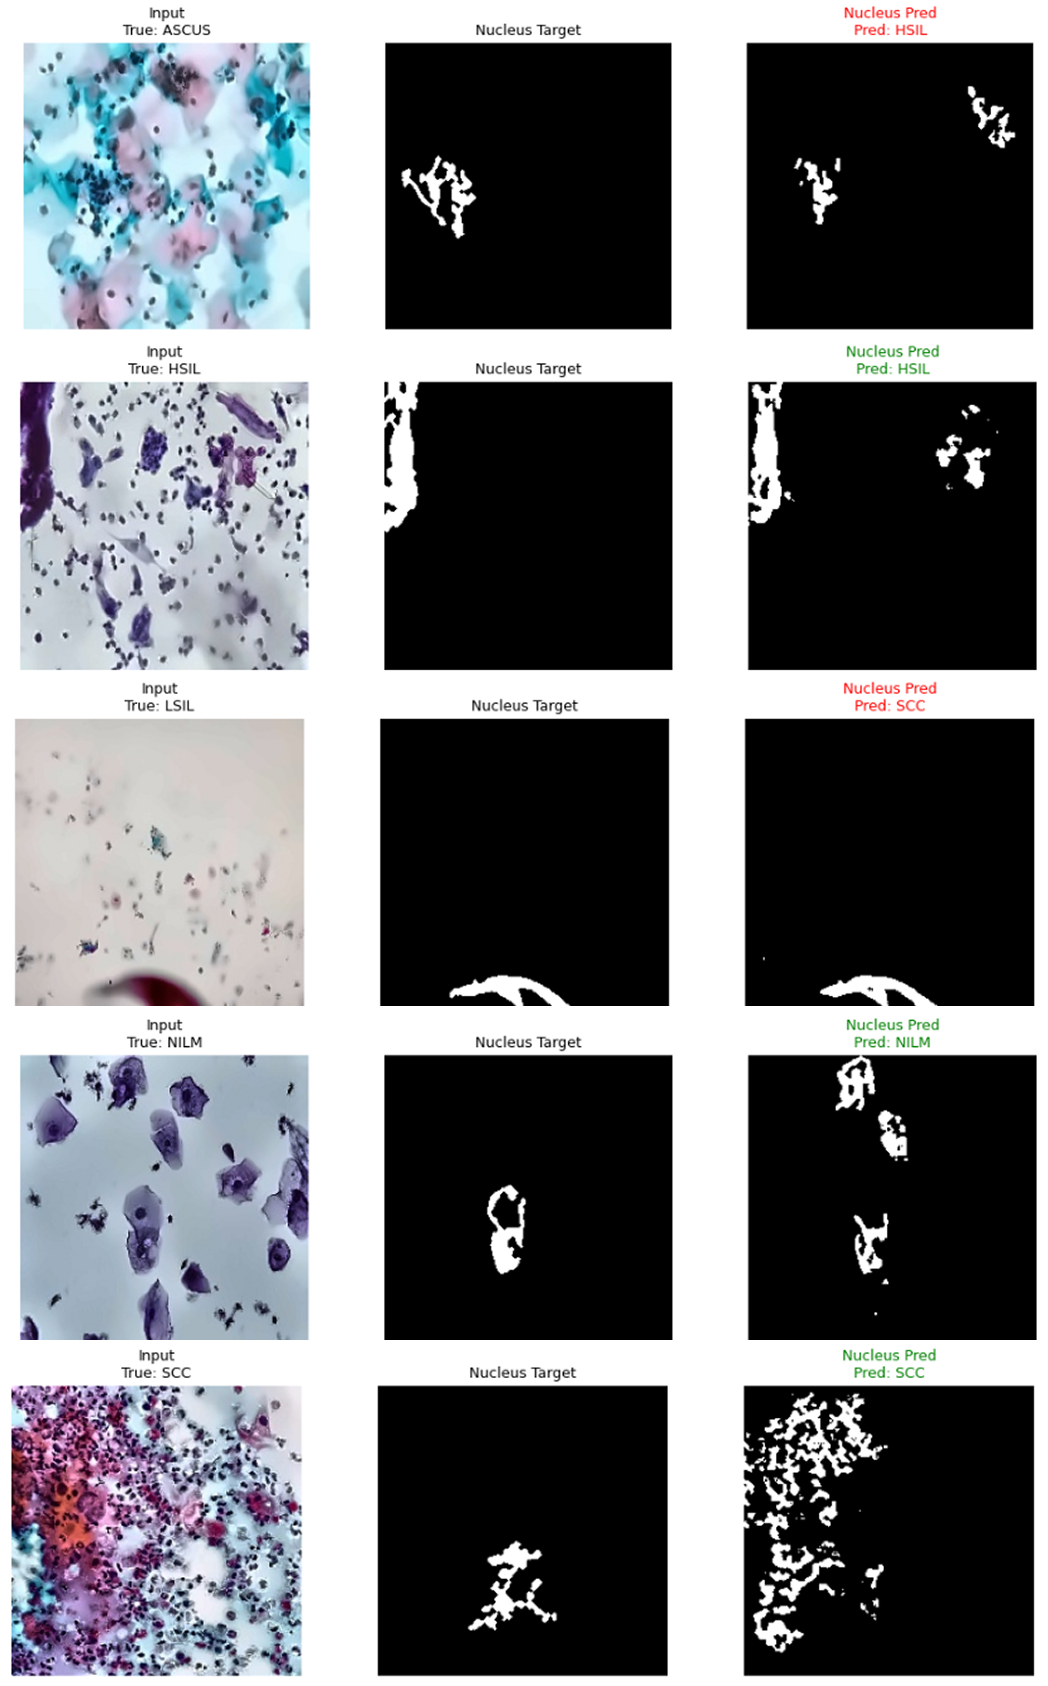
\includegraphics[width=\textwidth]{image/segmentation/cytology1Group 2.png}
        \caption{Cytology Dataset 1 (APCEM-Enhanced)}
        \label{fig:qual_ds1}
    \end{subfigure}
    
    \vspace{0.4cm}
    
    % Row 2
    \begin{subfigure}[b]{0.49\textwidth}
        \centering
        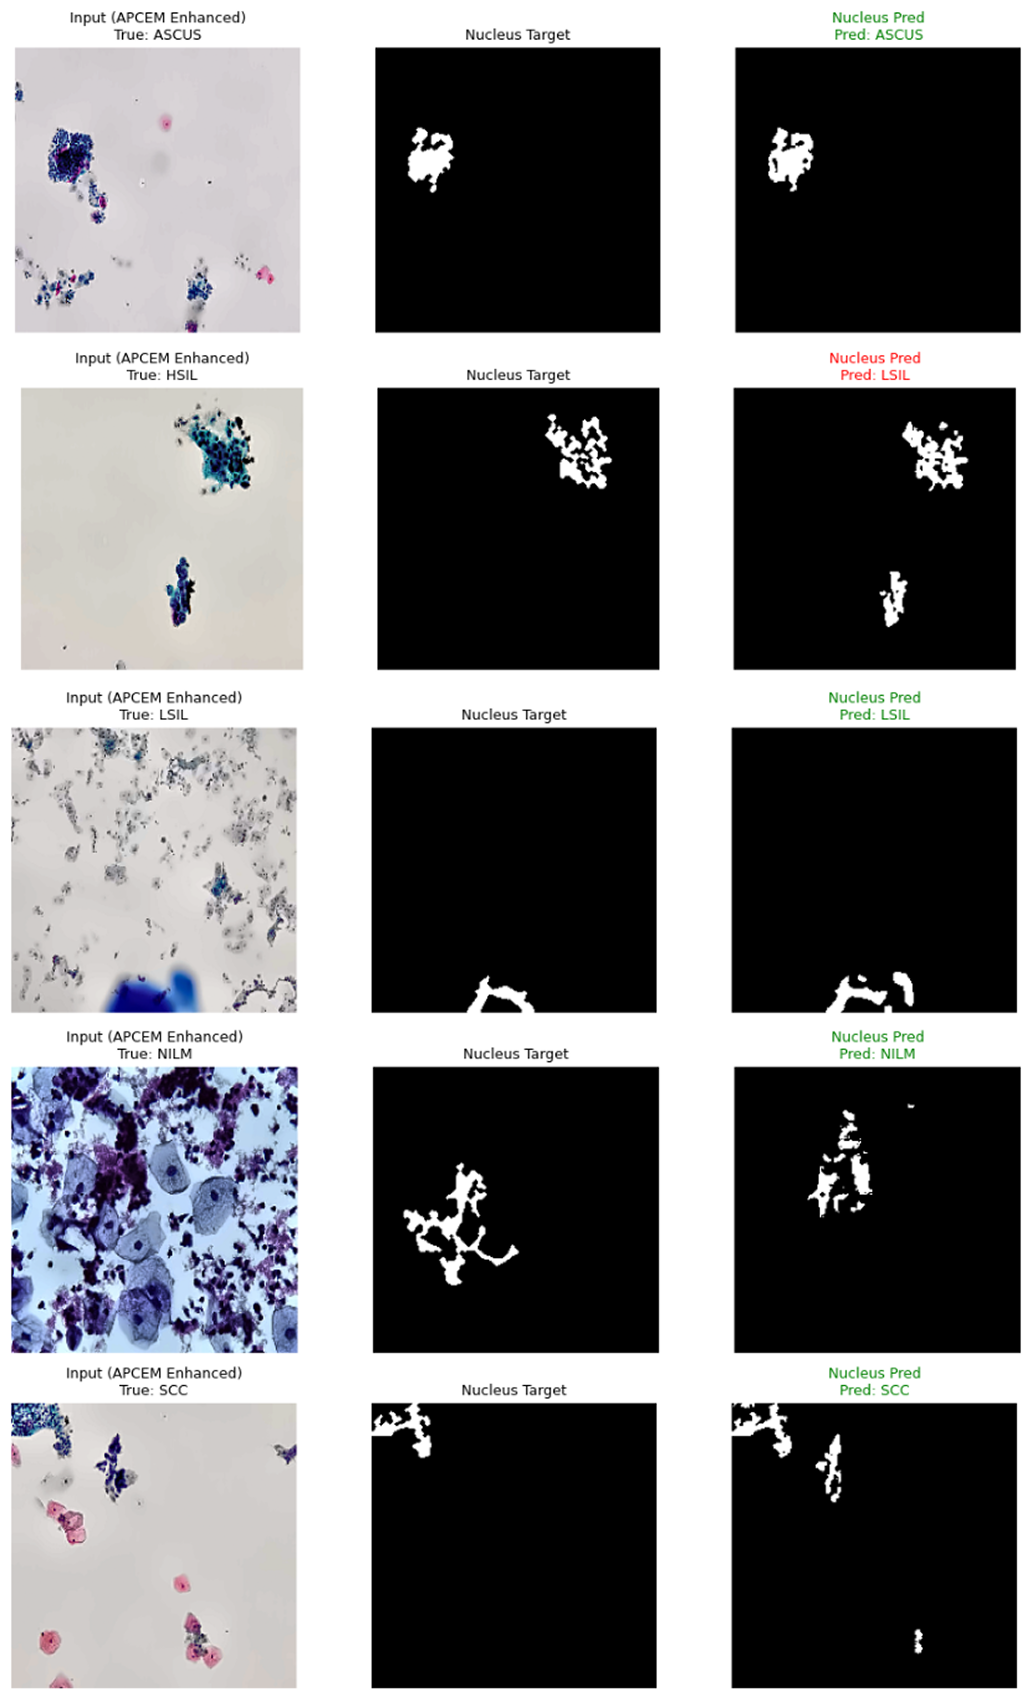
\includegraphics[width=\textwidth]{image/segmentation/cytology2Group 3.png}
        \caption{Cytology Dataset 2 (Raw with APCEM)}
        \label{fig:qual_ds2}
    \end{subfigure}
    \hfill
    \begin{subfigure}[b]{0.49\textwidth}
        \centering
        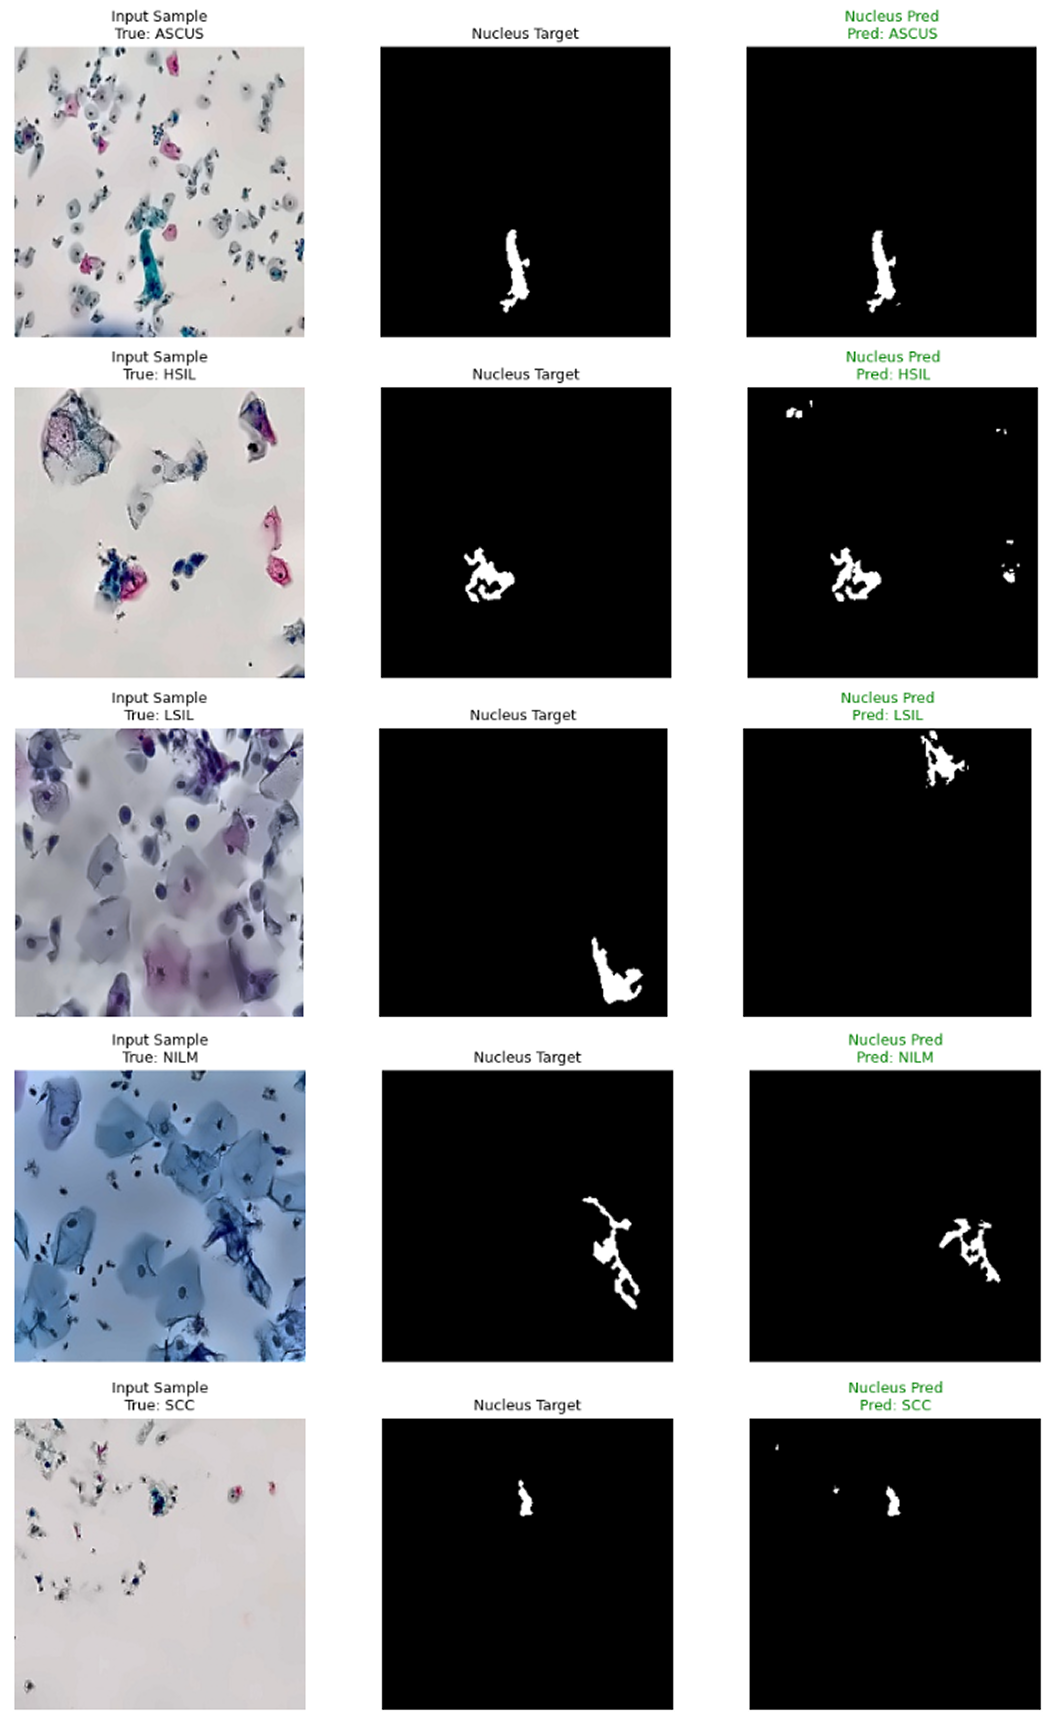
\includegraphics[width=\textwidth]{image/segmentation/Merge_Group 4.png}
        \caption{Merged Custom Cytology Dataset}
        \label{fig:qual_merged}
    \end{subfigure}
    \caption{Qualitative test sample predictions across all experimental cohorts. In each subfigure, samples are displayed as three-column triplets: (left) Input image, (middle) target nucleus mask (pathologist rasterized contour for SIPaKMeD; automated morphological pseudo-mask for cytology sets), and (right) predicted binary nucleus mask with diagnostic prediction (green title indicates correct classification; red indicates misclassification).}
    \label{fig:qualitative_segmentation_all}
\end{figure*}

\subsubsection{Qualitative Visual Inspection and Clinical Error Analysis}
To elucidate the performance disparity between the high Dice score on SIPaKMeD and the moderate scores on the cytology cohorts, representative inference triplets are visualized in Figure~\ref{fig:qualitative_segmentation_all}. A detailed qualitative analysis reveals several key clinical and technical insights:

\begin{enumerate}
    \item \textbf{High-Fidelity Contouring on Expert Ground Truth (SIPaKMeD):} 
    As depicted in Figure~\ref{fig:qual_sipak}, the framework exhibits exceptional boundary concordance on the SIPaKMeD benchmark. The predicted binary masks closely match the expert-delineated nuclear boundaries across diverse cytomorphological stages—from the small, condensed, pyknotic nuclei in normal superficial cells to the enlarged, irregularly lobulated nuclei seen in dysplastic koilocytes. The Multi-Head Self-Attention (MHSA) bottleneck allows the network to distinguish true nuclear chromatin from overlapping cytoplasmic folds and perinuclear halos, eliminating spurious mask leakage.

    \item \textbf{Pseudo-Mask Label Noise and Mathematical Over-Penalization:}
    Visual inspection of Cytology Dataset 1 (Figure~\ref{fig:qual_ds1}) and Dataset 2 (Figure~\ref{fig:qual_ds2}) shows that the lower test Dice scores ($\sim$45--49\%) are predominantly an artifact of noisy pseudo-ground-truth targets rather than localization failures by the network:
    \begin{itemize}
        \item The automated thresholding and morphological opening/closing pipeline frequently produces jagged, irregular, or partially hollow target masks when encountering chromatin vacuoles, uneven staining, or mucus strands.
        \item In contrast, the deep multi-task network acts as a robust spatial filter, predicting a smooth, continuous, and biologically plausible elliptical nucleus.
        \item When evaluating a smooth, anatomically correct predicted mask against a fragmented or jagged pseudo-target, the intersection area is reduced while the union expands, severely penalizing the Dice and IoU metrics despite the clinical superiority of the model's prediction.
    \end{itemize}

    \item \textbf{Robustness to Multi-Center Staining Variations:}
    On the Merged Custom Dataset (Figure~\ref{fig:qual_merged}), the network demonstrates strong resilience to severe illumination variations, diverse Papanicolaou counterstaining shades, and non-cellular background debris. Even in overlapping cellular clusters or out-of-focus preparations, the attention-enhanced representation accurately segments the primary dysplastic nucleus.

    \item \textbf{Mutual Synergism in Joint Multi-Task Learning:}
    Throughout the qualitative panels in Figure~\ref{fig:qualitative_segmentation_all}, test instances exhibiting accurate, well-circumscribed nuclear masks correspond almost uniformly to correct diagnostic classification calls (labeled in green text). Enforcing pixel-level nuclear boundary reconstruction serves as a powerful regularizer at the shared bottleneck, forcing the encoder to prioritize chromatin-rich regions while preventing the classification head from fitting to non-diagnostic background artifacts.
\end{enumerate}

\subsection{Confusion Matrix}

\subsubsection{Multi-class classification}

The performance and class-wise generalization of the proposed multi-task framework across different dataset configurations are quantitatively evaluated using confusion matrices, as illustrated in Figure~\ref{CM}.  

\begin{itemize}
    \item \textbf{Sipakmed Dataset (Figure \ref{fig:sub1_conf}):} The model shows an impressive discriminative ability on this dataset. Inter-class confusion is minimal, it predicts almost all the instances of Parabasal and Superficial\_intermediate classes. It mostly misclassified koilocytotic cells than others.   
\begin{figure}[htbp]
    \centering
    % First Row
    \begin{subfigure}[b]{0.48\textwidth}
        \centering
        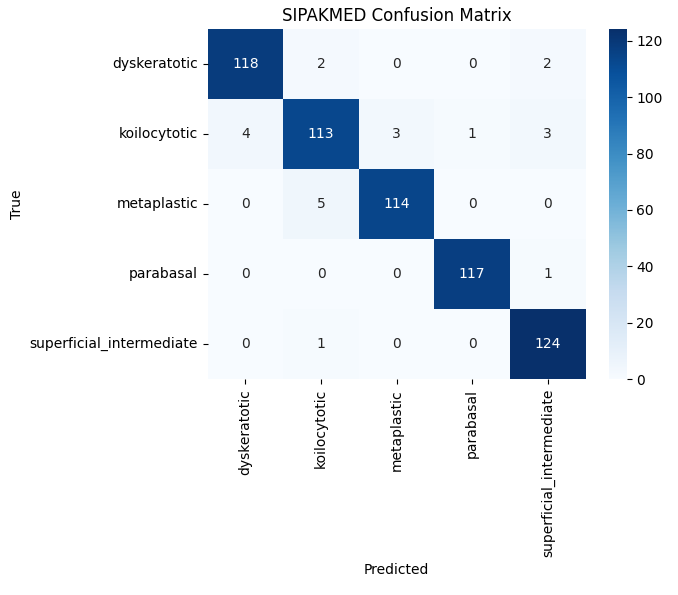
\includegraphics[width=\textwidth]{image/ConfusionMatrix/Multi/sipak.png} % Replace with your first image
        \caption{SipakMed}
        \label{fig:sub1_conf}
    \end{subfigure}
    \hfill
    \begin{subfigure}[b]{0.48\textwidth}
        \centering
        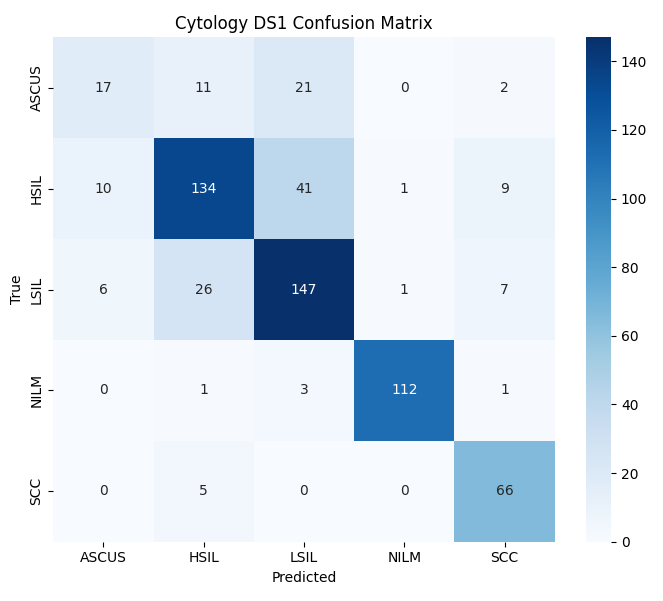
\includegraphics[width=\textwidth]{image/ConfusionMatrix/Multi/cytology1.png} % Replace with your second image
        \caption{APCEM-Enhanced Cervical Cytology}
        \label{fig:sub2_conf}
    \end{subfigure}

    \vspace{0.5cm} % Vertical space between rows

    % Second Row
    \begin{subfigure}[b]{0.48\textwidth}
        \centering
        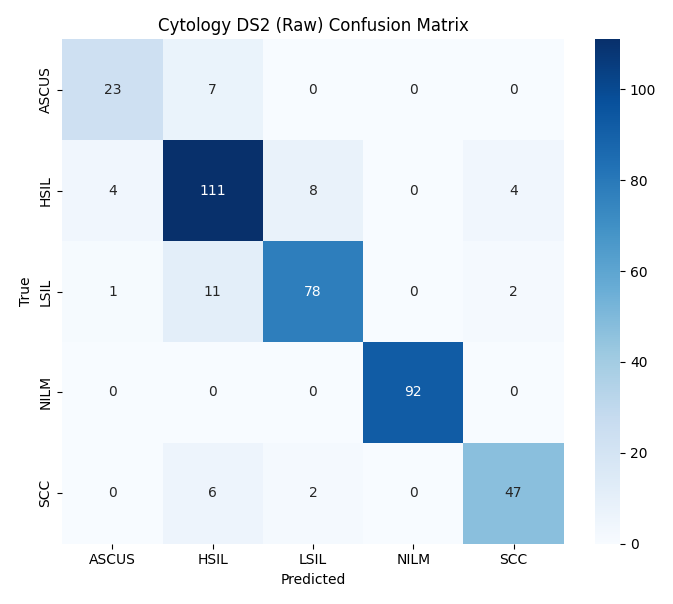
\includegraphics[width=\textwidth]{image/ConfusionMatrix/Multi/cytology2.png} % Replace with your third image
        \caption{CytologCervicalCancer}
        \label{fig:sub3_conf}
    \end{subfigure}
    \hfill
    \begin{subfigure}[b]{0.48\textwidth}
        \centering
        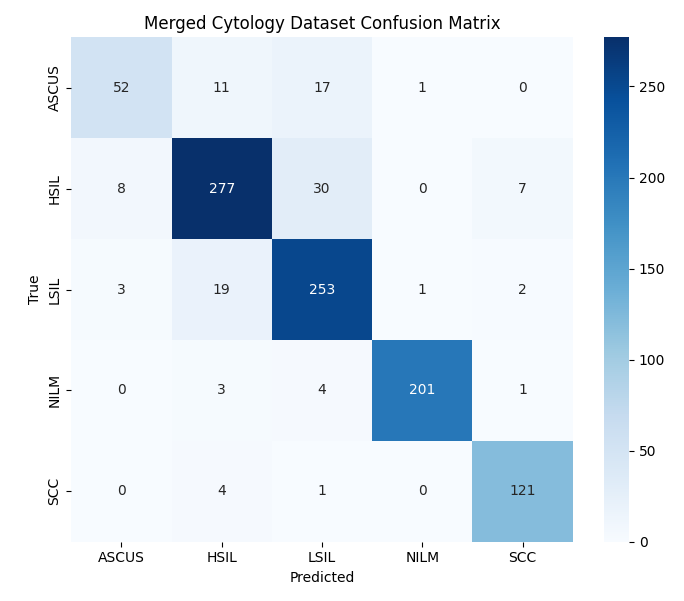
\includegraphics[width=\textwidth]{image/ConfusionMatrix/Multi/merge.png} % Replace with your fourth image
        \caption{Custom Dataset}
        \label{fig:sub4_conf}
    \end{subfigure}

    \caption{Confusion Matrix for Multi-Class Classification}
    \label{CM}
\end{figure}

\item \textbf{APCEM-Enhanced Cervical Cytology (Figure \ref{fig:sub2_conf}):} The framework reliably classified NILM class (117 correct predictions) and LSIL (147 correct predictions). However, the inherent morphological similarities among atypical and dysplastic cells introduce specific misclassifications; notably, 41 HSIL samples and 21 ASCUS samples are misclassified as LSIL. 

\item \textbf{CytologCervicalCancer (Figure \ref{fig:sub3_conf}):} The model exhibited strong predictive capabilities for high-grade lesions, correctly identifying 111 HSIL instances and all instances of NILM class. Model confused LSIL with the HSIL cell, as their differences are very less. 11 LSIL samples were misclassified as HSIL.

\item \textbf{Merged Custom Dataset (Figure \ref{fig:sub4_conf}):} Benefiting from the expanded spatial diversity and sample size, the merged dataset yields robust true positive concentrations for the most critical diagnostic categories, successfully classifying 277 HSIL, 253 LSIL, 201 NILM, and 121 SCC instances. While the complex diagnostic boundaries between mild and severe dysplasia result in some bidirectional overlap (30 HSIL cases predicted as LSIL, and 19 LSIL cases predicted as HSIL). \\

\end{itemize}
 

\subsubsection{Binary Classification}

Confusion matrices in Figure~\ref{CM_binary} represent the quantitative result of the proposed model for binary classification. 

\begin{itemize}
    \item \textbf{Sipakmed Dataset (Figure~\ref{fig:first_image}):} The model demonstrates very reliable discriminative abilities on the SIPaKMeD dataset. It shows a high sensitivity to pathological cellular changes by correctly identifying 236 normal and 359 abnormal instances. Misclassifications are extremely low and balanced, with only 7 normal samples labeled as abnormal (false positives) and six abnormal samples predicted as normal (false negatives).

    \begin{figure}[htbp]
    \centering
    % First Subfigure
    \begin{subfigure}[b]{0.48\textwidth}
        \centering
        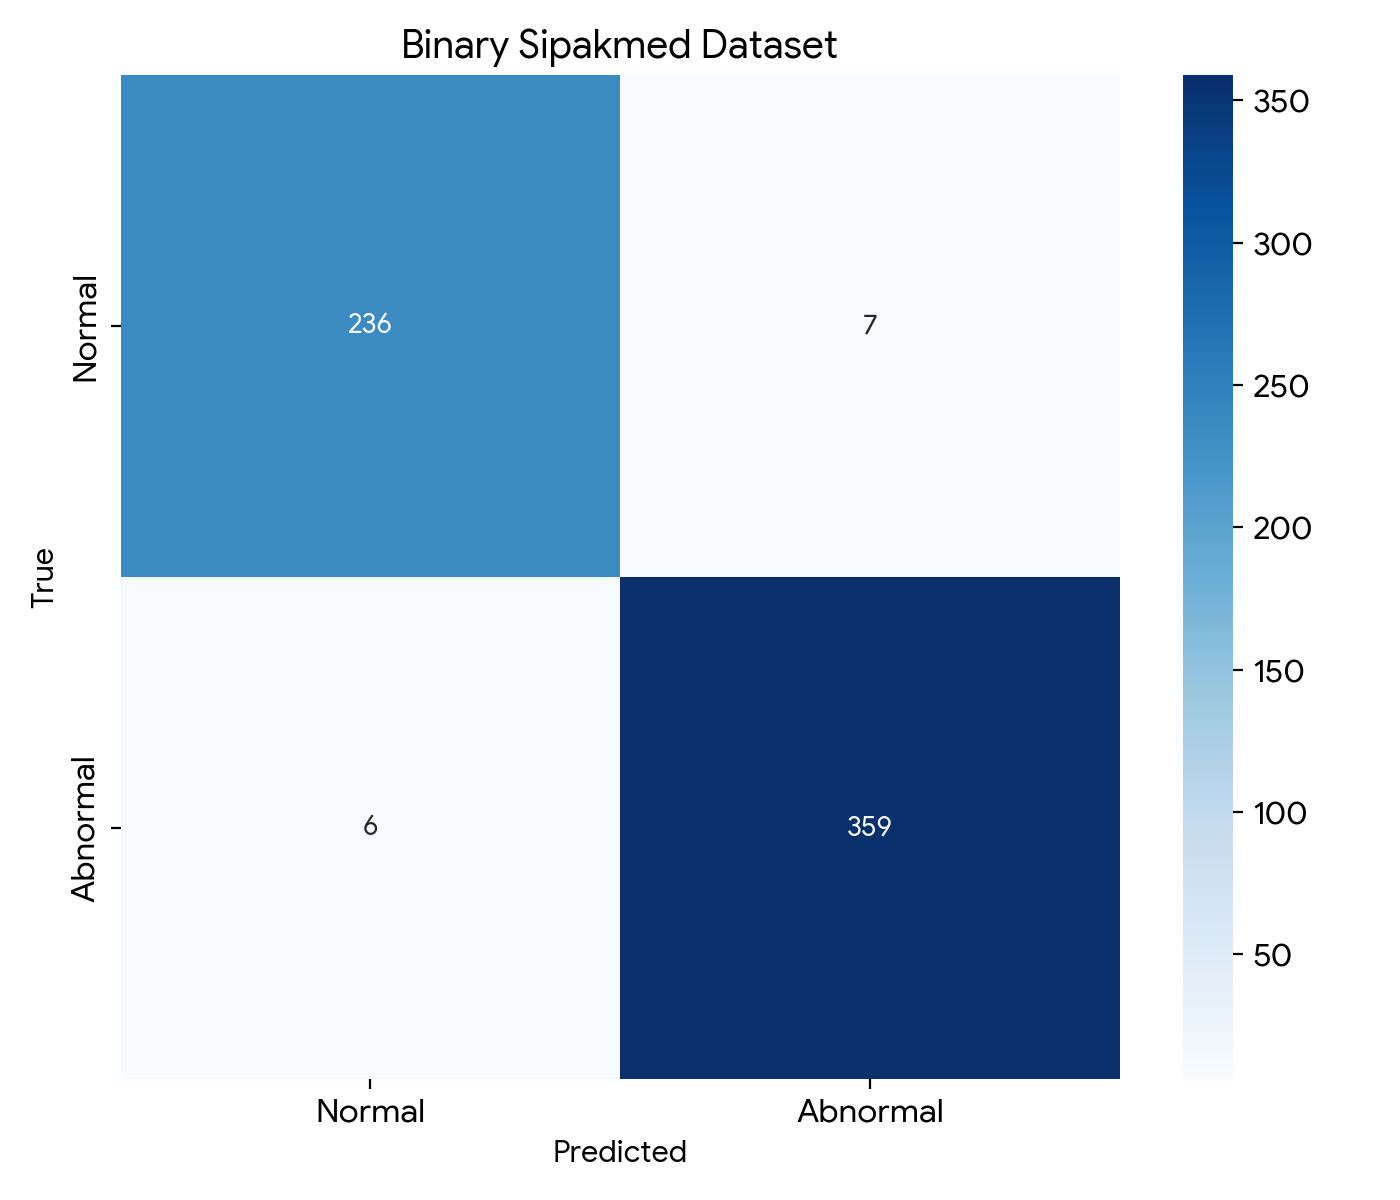
\includegraphics[width=\textwidth]{image/ConfusionMatrix/binary/sipak.png} % Replace with your first image path
        \caption{Sipakmed Dataset}
        \label{fig:first_image}
    \end{subfigure}
    \hfill % Adds horizontal space between the two images
    % Second Subfigure
    \begin{subfigure}[b]{0.48\textwidth}
        \centering
        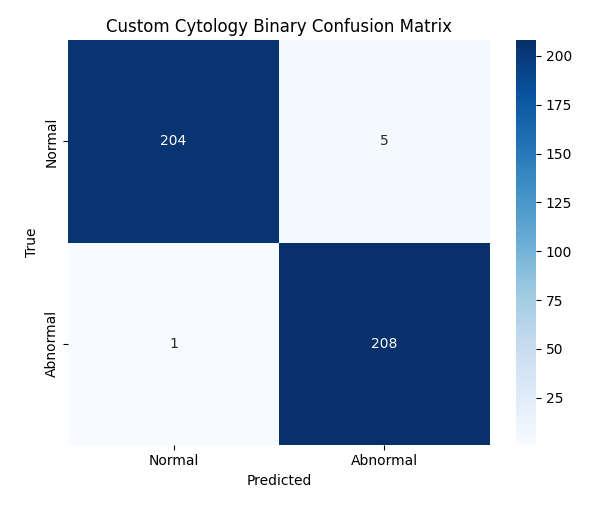
\includegraphics[width=\textwidth]{image/ConfusionMatrix/binary/custom.png} % Replace with your second image path
        \caption{Custom Binary Cytology Dataset}
        \label{fig:second_image}
    \end{subfigure}
    
    \caption{Confusion Matrix for Binary Class Classification}
    \label{CM_binary}
\end{figure}

\item \textbf{Merged Custom Dataset (Figure~\ref{fig:second_image}):} The system achieves high diagnostic precision when tested on the custom dataset. 204 normal instances and 208 abnormal instances are effectively identified. Most significantly, only one abnormal cell is incorrectly classified as normal by the model, resulting in an exceptionally low false-negative rate. This minimization of false negatives is a critical performance metric for automated cervical cancer screening, ensuring that no malignant cases are overlooked by the model, while maintaining a minimal false-positive count of just 5 instances.
    
\end{itemize}


\subsection{Ablation Study}

To isolate the contribution of the architectural modifications proposed in this work, we conducted a ablation study comparing two variants of the Multi-Task Residual-Attention Network: Model 1 (baseline), which uses a plain (non-residual) \textbf{DoubleConv} block and a single GAP-based classification head, and Model 2 (proposed), which introduces (i) residual shortcut connections within every convolutional block, (ii) spatial dropout (Dropout2d, 0.15/0.20) in the deeper encoder stages, and (iii) a dual-pooling (GAP+GMP) classification head. All other components—the self-attention bottleneck, the encoder/decoder topology, channel configuration, and training procedure—were held identical between the two variants to ensure a controlled comparison. Both models were trained and evaluated under same conditions across six dataset configurations: the five-class SIPaKMeD dataset, the APCEM-enhanced dataset, the CytologCervicalCancer dataset, the custom merged (APCEM + CytologCervicalCancer) multi-class dataset, the binary SIPaKMeD dataset, and the custom binary merged dataset. Here, the evaluation matrices—precision, recall, and f1-score are weighted-averaged across classes.

\begin{table}[htbp]
\centering
\caption{Ablation study comparing the \textbf{baseline model (Model 1)} against the \textbf{proposed model (Model 2)} across all evaluated dataset configurations.}
\label{tab:ablation_study}
\begin{tabular}{p{3.0cm} p{1.25cm} ccccc}
\toprule
\textbf{Dataset} & \textbf{Model} & \textbf{Accuracy (\%)} & \textbf{Dice Score} & \textbf{Precision} & \textbf{Recall} & \textbf{F1-Score} \\
\midrule

\multirow{2}{*}{\parbox{3.0cm}{SIPaKMeD (5-class)}}
 & Model 1 & 94.90 & 0.8264 & 0.95 & 0.95 & 0.95 \\
 & \textbf{Model 2} & \textbf{96.38} & \textbf{0.8646} & \textbf{0.96} & \textbf{0.96} & \textbf{0.96} \\
\midrule

\multirow{2}{*}{\parbox{3.0cm}{APCEM-Enhanced}}
 & Model 1 & 72.46 & 0.4466 & 0.73 & 0.72 & 0.72 \\
 & \textbf{Model 2} & \textbf{76.65} & \textbf{0.4519} & \textbf{0.76} & \textbf{0.77} & \textbf{0.76} \\
\midrule

\multirow{2}{*}{\parbox{3.0cm}{CytologCervicalCancer}}
 & Model 1 & 74.75 & \textbf{0.4930} & 0.76 & 0.75 & 0.75 \\
 & \textbf{Model 2} & \textbf{88.64} & 0.4917 & \textbf{0.89} & \textbf{0.89} & \textbf{0.89} \\
\midrule

\multirow{2}{*}{\parbox{3.0cm}{Custom Cervical Cytology (Multi)}}
 & Model 1 & 81.79 & 0.4881 & 0.82 & 0.82 & 0.81 \\
 & \textbf{Model 2} & \textbf{88.98} & \textbf{0.4998} & \textbf{0.89} & \textbf{0.89} & \textbf{0.89} \\
\midrule

\multirow{2}{*}{\parbox{3.0cm}{SIPaKMeD (Binary)}}
 & Model 1 & 97.04 & 0.8357 & 0.97 & 0.97 & 0.97 \\
 & \textbf{Model 2} & \textbf{97.86} & \textbf{0.8801} & \textbf{0.98} & 0.98 & \textbf{0.98} \\
\midrule

\multirow{2}{*}{\parbox{3.2cm}{Custom Cervical Cytology (Binary)}}
 & Model 1 & 97.85 & \textbf{0.4337} & 0.98 & 0.98 & 0.98 \\
 & \textbf{Model 2} & \textbf{98.56} & 0.4230 & \textbf{0.99} & \textbf{0.99} & \textbf{0.99} \\

\bottomrule
\end{tabular}
\end{table}

% \begin{table}[htbp]
% \centering
% \caption{Ablation study comparing the baseline model (Model 1) against the proposed model (Model 2) across all evaluated dataset configurations.}
% \label{tab:ablation_study}
% \begin{tabularx}{\textwidth}{L ccccc}
% \toprule
% \textbf{Model Configuration} & \textbf{Accuracy (\%)} & \textbf{Dice Score} & \textbf{Precision} & \textbf{Recall} & \textbf{F1-Score} \\
% \midrule

% \multicolumn{6}{l}{\textbf{SIPaKMeD (5-class)}} \\
% \hspace{1em} Model 1 (Baseline) & 94.90 & 0.8264 & 0.95 & 0.95 & 0.95 \\
% \hspace{1em} \textbf{Model 2 (Proposed)} & \textbf{96.38} & \textbf{0.8646} & \textbf{0.96} & \textbf{0.96} & \textbf{0.96} \\
% \midrule

% \multicolumn{6}{l}{\textbf{APCEM-Enhanced}} \\
% \hspace{1em} Model 1 (Baseline) & 72.46 & 0.4466 & 0.73 & 0.72 & 0.72 \\
% \hspace{1em} \textbf{Model 2 (Proposed)} & \textbf{76.65} & \textbf{0.4519} & \textbf{0.76} & \textbf{0.77} & \textbf{0.76} \\
% \midrule

% \multicolumn{6}{l}{\textbf{CytologCervicalCancer}} \\
% \hspace{1em} Model 1 (Baseline) & 74.75 & \textbf{0.4930} & 0.76 & 0.75 & 0.75 \\
% \hspace{1em} \textbf{Model 2 (Proposed)} & \textbf{88.64} & 0.4917 & \textbf{0.89} & \textbf{0.89} & \textbf{0.89} \\
% \midrule

% \multicolumn{6}{l}{\textbf{Custom Cervical Cytology Dataset (Multi-Class)}} \\
% \hspace{1em} Model 1 (Baseline) & 81.79 & 0.4881 & 0.82 & 0.82 & 0.81 \\
% \hspace{1em} \textbf{Model 2 (Proposed)} & \textbf{88.98} & \textbf{0.4998} & \textbf{0.89} & \textbf{0.89} & \textbf{0.89} \\
% \midrule

% \multicolumn{6}{l}{\textbf{SIPaKMeD (Binary)}} \\
% \hspace{1em} Model 1 (Baseline) & 97.04 & 0.8357 & 0.97 & 0.97 & 0.97 \\
% \hspace{1em} \textbf{Model 2 (Proposed)} & \textbf{97.86} & \textbf{0.8801} & \textbf{0.98} & 0.98 & \textbf{0.98} \\
% \midrule

% \multicolumn{6}{l}{\textbf{Custom Cervical Cytology Dataset (Binary)}} \\
% \hspace{1em} Model 1 (Baseline) & 97.85 & \textbf{0.4337} & 0.98 & 0.98 & 0.98 \\
% \hspace{1em} \textbf{Model 2 (Proposed)} & \textbf{98.56} & 0.4230 & \textbf{0.99} & \textbf{0.99} & \textbf{0.99} \\

% \bottomrule
% \end{tabularx}
% \end{table}

% \begin{table}[htbp]
% \centering
% \caption{Ablation study comparing the baseline model (Model 1) against the proposed model (Model 2) across all evaluated dataset configurations.}
% \label{tab:ablation_study}
% \resizebox{\textwidth}{!}{%
% \begin{tabular}{llccccc}
% \toprule
% \textbf{Dataset} & \textbf{Model} & \textbf{Accuracy (\%)} & \textbf{Dice Score} & \textbf{Precision} & \textbf{Recall} & \textbf{F1-Score} \\
% \midrule

% \multirow{2}{*}{SIPaKMeD (5-class)}
%  & Model 1 (Baseline) & 94.90 & 0.8264 & 0.95 & 0.95 & 0.95 \\
%  & \textbf{Model 2 (Proposed)} & \textbf{96.38} & \textbf{0.8646} & \textbf{0.96} & \textbf{0.96} & \textbf{0.96} \\
% \midrule

% \multirow{2}{*}{APCEM-Enhanced}
%  & Model 1 (Baseline) & 72.46 & 0.4466 & 0.73 & 0.72 & 0.72 \\
%  & \textbf{Model 2 (Proposed)} & \textbf{76.65} & \textbf{0.4519} & \textbf{0.76} & \textbf{0.77} & \textbf{0.76} \\
% \midrule

% \multirow{2}{*}{CytologCervicalCancer}
%  & Model 1 (Baseline) & 74.75 & \textbf{0.4930} & 0.76 & 0.75 & 0.75 \\
%  & \textbf{Model 2 (Proposed)} & \textbf{88.64} & 0.4917 & \textbf{0.89} & \textbf{0.89} & \textbf{0.89} \\
% \midrule

% \multirow{2}{*}{Custom Cervical Cytology Dataset(Multi)}
%  & Model 1 (Baseline) & 81.79 & 0.4881 & 0.82 & 0.82 & 0.81 \\
%  & \textbf{Model 2 (Proposed)} & \textbf{88.98} & \textbf{0.4998} & \textbf{0.89} & \textbf{0.89} & \textbf{0.89} \\
% \midrule

% \multirow{2}{*}{SIPaKMeD (Binary)}
%  & Model 1 (Baseline) & 97.04 & 0.8357 & 0.97 & 0.97 & 0.97 \\
%  & \textbf{Model 2 (Proposed)} & \textbf{97.86} & \textbf{0.8801} & \textbf{0.98} & 0.98 & \textbf{0.98} \\
% \midrule

% \multirow{2}{*}{Custom Cervical Cytology Dataset (Binary)}
%  & Model 1 (Baseline) & 97.85 & \textbf{0.4337} & 0.98 & 0.98 & 0.98 \\
%  & \textbf{Model 2 (Proposed)} & \textbf{98.56} & 0.4230 & \textbf{0.99} & \textbf{0.99} & \textbf{0.99} \\

% \bottomrule
% \end{tabular}%
% }
% \end{table}

The ablation results in Table~\ref{tab:ablation_study} confirm that residual connections, spatial dropout, and the dual-pooling head consistently boost classification accuracy. This improvement is especially pronounced on challenging, class-imbalanced datasets compared to SIPaKMeD. On the other hand, modest segmentation gains across datasets support our hypothesis that mask quality is bottlenecked by pseudo-label noise rather than backbone capacity. Overall, these findings validate our design choices. They also show that future improvements, particularly for minority classes like ASCUS, will come from tackling class imbalance and refining mask generation rather than further tweaking the backbone.

\section{Comparative Analysis}
\label{sec:comparative_analysis}

To rigorously assess the performance of the proposed multi-task architecture against established literature, we conducted an empirical benchmark on the five-class SIPaKMeD dataset. The comparative cohort encompasses four prominent deep learning architectures tailored for cervical cytology classification alongside our proposed framework and its ablation baseline. Specifically, the external benchmarks include a dual-backbone transfer learning framework combining ResNet-50 and VGG-19 feature fusion~\cite{sharma2025diagnosis}, a hybrid multi-scale network fusing Inception-v3 and DenseNet-201 representations~\cite{sharma2025enhancing}, a soft-voting ensemble comprising five distinct CNN backbones (ResNet-50, VGG-16, MobileNet-V2, DenseNet-121, and EfficientNet-B0)~\cite{Verma2025}, and the lightweight Multi-Resolution Fusion Deep Convolutional Network (MRF-DCN) utilizing multi-scale depthwise separable convolutions~\cite{shaik2025deeplearningenabledsegmentation}. These benchmark systems are evaluated alongside our internal baseline architecture lacking residual shortcuts and utilizing a single global average pooling head (Model~1), as well as the proposed attention-enhanced multi-task network incorporating residual connections and a dual-pooling classification head (Model~2).

\noindent \textbf{Fair Evaluation and Experimental Rigor:} In biomedical image analysis, directly transcribing performance figures from published literature frequently yields skewed comparisons due to divergent preprocessing steps, disparate train/validation/test split ratios, data leakage, or private augmentation strategies. Therefore, to guarantee a strictly controlled, unbiased, and reproducible benchmark, none of the performance metrics presented in Table~\ref{tab:model_comparison} were transcribed from their original publications. Instead, all baseline models were faithfully re-implemented in PyTorch according to their published architectural specifications, initialized with identical random seeds, and independently trained and evaluated locally under the exact same stratified $70\%/15\%/15\%$ split, input resolution ($224 \times 224$), optimization routine, and evaluation protocols described in Section~\ref{sec:method}.

% \begin{table}[htbp]
%     \centering
%     \caption{Model Performance Comparison with existing model for Sipakmed Multi-class classification}
%     \label{tab:model_comparison}
%     \resizebox{\textwidth}{!}{%
%     \begin{tabular}{lcccc}
%         \toprule
%         \textbf{Model} & \textbf{Accuracy} & \textbf{Precision} & \textbf{Recall} & \textbf{F1 Score} \\
%         \midrule
%         Transfer learning(ResNet50 and VGG19)~\cite{sharma2025diagnosis}& 96.02 & 96.02 & 96.02 & 95.98 \\
%         InceptionV3 + DenseNet201~\cite{sharma2025enhancing} & 97.08 & 97.14 & 97.08 & 97.07 \\
%         Ensemble of 5 CNN model~\cite{Verma2025} & 96.41 & 96.45 & 96.41 & 96.40 \\
%         MRF-DCN~\cite{shaik2025deeplearningenabledsegmentation} & 94.95 & 94.97 & 94.95 & 94.94 \\
%         Proposed Model without Residual Network & 94.90 & 95 & 95 & 95 \\
%         Proposed Model with Residual Network & \textbf{96.38} & \textbf{96} & \textbf{96} & \textbf{96} \\
%         \bottomrule
%     \end{tabular}%
%     }
% \end{table}

\begin{table}[htbp]
\centering
\caption{Empirical benchmark comparison on the SIPaKMeD five-class dataset. All baseline models were independently re-implemented, retrained, and tested on identical data splits under the same experimental conditions.}
\label{tab:model_comparison}
\setlength{\tabcolsep}{2.5pt} % Tightens inter-column padding to accommodate full header labels
\begin{tabular}{>{\raggedright\arraybackslash}p{4.0cm} ccccc}
\toprule
\textbf{Model Architecture} & \textbf{Params} & \textbf{Accuracy (\%)} & \textbf{Precision (\%)} & \textbf{Recall (\%)} & \textbf{F1 Score (\%)} \\
\midrule
Transfer learning (ResNet50 + VGG19)~\cite{sharma2025diagnosis} & $\sim$44.60\,M & 96.02 & 96.02 & 96.02 & 95.98 \\
InceptionV3 + DenseNet201~\cite{sharma2025enhancing}             & $\sim$43.80\,M & 97.08 & 97.14 & 97.08 & 97.07 \\
Ensemble of 5 CNN models~\cite{Verma2025}                        & $\sim$180.80\,M & 96.41 & 96.45 & 96.41 & 96.40 \\
MRF-DCN~\cite{shaik2025deeplearningenabledsegmentation}         & $\sim$0.85\,M  & 94.95 & 94.97 & 94.95 & 94.94 \\
Proposed Model w/o Residuals (Model 1)                          & 2.37\,M        & 94.90 & 95.00 & 95.00 & 95.00 \\
\textbf{Proposed Multi-Task Net (Model 2)}                      & \textbf{2.41\,M} & \textbf{96.38} & \textbf{96.00} & \textbf{96.00} & \textbf{96.00} \\
\bottomrule
\end{tabular}
\end{table}

% \begin{table}[htbp]
% \caption{Empirical benchmark comparison on the SIPaKMeD five-class dataset. All baseline models were independently re-implemented, retrained, and tested on identical data splits under the same experimental conditions.}
% \label{tab:model_comparison}
% \begin{tabularx}{\textwidth}{>{\raggedright\arraybackslash}X ccccc}
% \toprule
% \textbf{Model Architecture} & \textbf{Params (M)} & \textbf{Accuracy (\%)} & \textbf{Precision (\%)} & \textbf{Recall (\%)} & \textbf{F1 Score (\%)} \\
% \midrule
% Transfer learning (ResNet50 + VGG19)~\cite{sharma2025diagnosis} & $\sim$44.60\,M & 96.02 & 96.02 & 96.02 & 95.98 \\
% InceptionV3 + DenseNet201~\cite{sharma2025enhancing}             & $\sim$43.80\,M & 97.08 & 97.14 & 97.08 & 97.07 \\
% Ensemble of 5 CNN models~\cite{Verma2025}                        & $\sim$180.80\,M & 96.41 & 96.45 & 96.41 & 96.40 \\
% MRF-DCN~\cite{shaik2025deeplearningenabledsegmentation}         & $\sim$0.85\,M  & 94.95 & 94.97 & 94.95 & 94.94 \\
% Proposed Model without Residuals (Model 1)                       & 2.37\,M        & 94.90 & 95.00 & 95.00 & 95.00 \\
% \textbf{Proposed Multi-Task Net (Model 2)}                      & \textbf{2.41\,M} & \textbf{96.38} & \textbf{96.00} & \textbf{96.00} & \textbf{96.00} \\
% \bottomrule
% \end{tabularx}
% \end{table}

The quantitative findings, compiled in Table 17, highlight several vital architectural and clinical trade-offs:
\begin{itemize}
    \item \textbf{Performance vs. Parameter Scale:} The hybrid InceptionV3 + DenseNet201 framework~\cite{sharma2025enhancing} and the five-model ensemble~\cite{Verma2025} achieved marginal accuracy leads ($97.08\%$ and $96.41\%$, respectively) compared to our proposed network ($96.38\%$). However, these marginal gains require an immense computational overhead: InceptionV3 + DenseNet201 utilizes $\sim$43.80\,M parameters (over \textbf{$18\times$ larger}), while the five-backbone ensemble requires $\sim$180.80\,M parameters (\textbf{$75\times$ larger} than our proposed $2.41$\,M parameter model). In clinical edge deployment and automated screening microscopes, such massive parameter scaling creates severe latency and memory bottlenecks with diminishing diagnostic returns.
    \item \textbf{Limitations of Ultra-Compact Networks:} Conversely, while the MRF-DCN architecture~\cite{shaik2025deeplearningenabledsegmentation} minimizes parameter footprint ($\sim$0.85\,M parameters), its constrained depthwise convolutions exhibit lower discriminative capability, achieving $94.95\%$ accuracy and struggling to differentiate subtle morphological overlaps between dyskeratotic and koilocytotic cells.
    \item \textbf{Multi-Task Diagnostic Superiority:} Crucially, all four external baselines~\cite{sharma2025diagnosis, sharma2025enhancing, Verma2025, shaik2025deeplearningenabledsegmentation} function solely as classification models, outputting a discrete diagnostic label without spatial interpretability. In contrast, our proposed framework ($2.41$\,M parameters) simultaneously achieves competitive five-class classification ($96.38\%$) and high-fidelity pixel-level nucleus segmentation ($86.46\%$ test Dice score) in a single unified forward pass. The synergistic multi-task learning constraint enables our compact network to match or approach the performance of massive ensemble systems while providing clinicians with verifiable nuclear segmentations.
\end{itemize}

To the best of our knowledge, no prior literature has reported standardized benchmark evaluations on the APCEM-Enhanced Cervical Cytology~\cite{aswini2026apcem}, CytologCervicalCancer~\cite{jnx03_2025}, or the combined Custom Merged dataset under a unified five-class Bethesda categorization and joint nucleus segmentation framework. Consequently, direct comparative evaluation against published external architectures on these cohorts is not currently feasible. The empirical findings documented in this work establish the foundational performance baselines for these datasets, providing a standardized point of reference to facilitate fair and rigorous comparisons for future automated cervical cytology studies.



\section{Discussion}\label{sec6}



Automated cervical cancer screening requires both categorical diagnostic triage and explainable morphological localization. The results presented in this work demonstrate that unifying nucleus segmentation and cell classification within an attention-guided multi-task learning (MTL) architecture yields superior diagnostic stability compared to isolated single-task paradigms.

\subsection{Morphological Regularization via Multi-Task Learning}
According to the Bethesda System for Reporting Cervical Cytology, the malignant transformation of cervical squamous epithelium is biologically heralded by nuclear alterations: progressive enlargement, coarse chromatin clumpiness, nuclear membrane irregularization, and elevation of the nuclear-to-cytoplasmic (N/C) ratio. In conventional single-task classification networks, encoders often suffer from "shortcut learning," where decision boundaries are influenced by irrelevant background slide debris, mucus, or illumination gradients. By enforcing joint pixel-level nucleus mask reconstruction through a shared bottleneck, our framework establishes an intrinsic spatial regularizer: the encoder is forced to preserve high-frequency chromatin boundary representations. As observed in the qualitative triplets (Figure~\ref{fig:qualitative_segmentation_all}), test samples with high segmentation fidelity exhibit almost flawless diagnostic classification, validating that spatial nuclear localization directly strengthens discriminative class feature extraction.

\subsection{Resolving the Ground-Truth vs. Pseudo-Mask Divergence}
A prominent observation in our empirical findings is the numerical discrepancy between the nucleus segmentation Dice score on SIPaKMeD (86.46\%) and those achieved on the cytology datasets (45.19\% on APCEM-Enhanced, 49.17\% on CytologCervicalCancer, and 54.44\% on the Merged Custom Dataset). A superficial reading might suggest underperformance of the segmentation branch on cytology cohorts; however, our qualitative error analysis reveals a "pseudo-annotation penalty":
\begin{enumerate}
    \item \textbf{Heuristic Label Noise vs. Deep Continuous Prior:} The automated thresholding and morphological extractor used on the cytology cohorts often yields fragmented, hollow, or boundary-jagged masks due to hyperchromatic vacuoles and stain intensity non-uniformity. In contrast, the Res-UNet branch, guided by spatial convolution and multi-head self-attention, outputs smooth, continuous, anatomically coherent nuclear boundaries.
    \item \textbf{Mathematical Asymmetry of Overlap Metrics:} Evaluating an anatomically correct, convex elliptical prediction against a concave or fractured pseudo-mask severely depresses the intersection numerator in the Dice formulation ($2|X \cap Y| / (|X| + |Y|)$), artificially penalizing the quantitative score despite superior clinical utility.
    \item \textbf{Cross-Center Synergistic Gains:} Merging the two cytology cohorts yielded an absolute gain of $+9.25\%$ in Dice over APCEM alone, proving that exposing the segmentation head to multi-center counterstains regularizes boundary prediction across scanner profiles.
\end{enumerate}

\subsection{Diagnostic Challenges in Equivocal Lesions (ASCUS)}
Across all cytology cohorts, the ASCUS category recorded the lowest sensitivity (recall of 0.33 in APCEM, improved to 0.64 in the Merged Custom Dataset). This behavior directly mirrors clinical cytopathology. Under Bethesda guidelines, ASCUS represents an equivocal, borderline category where cytomorphological changes suggestive of Low-Grade Squamous Intraepithelial Lesions (LSIL) are quantitatively or qualitatively insufficient for a definitive diagnosis. Pathologists themselves exhibit substantial inter-observer variability when categorizing ASCUS, with clinical concordance often lingering between 40\% and 60\%. In our experiments, misclassified ASCUS samples were predominantly routed into LSIL or NILM, confirming that the network encounters the identical borderline ambiguities documented in clinical practice. The substantial recovery of ASCUS F1-score from 0.40 on APCEM to 0.72 on the merged dataset highlights that data curation and multi-center diversity are critical for stabilizing equivocal diagnostic boundaries.

\subsection{Architectural Synergy and Ablation Insights}
The ablation study (Table~\ref{tab:ablation_study}) confirms that both the residual DoubleConv blocks and the dual-pooling (GAP + GMP) classification head are pivotal. Global Average Pooling (GAP) provides an invariant summary of spatial activation density, while Global Max Pooling (GMP) preserves sharp, localized feature spikes characteristic of severe chromatin condensation or abnormal nucleoli. Combining both pooling vectors expands the representation capacity from 256 to 512 dimensions without inflating convolutional parameter depth, contributing directly to the jump in classification accuracy observed in CytologCervicalCancer (from 74.75\% to 88.64\%). Concurrently, the bottleneck MHSA module captures wide-angle context across the $28 \times 28$ feature grid, enabling the network to calibrate cell-level cytoplasmic proportions against the localized nuclear core.


\section{Limitations and Future Work}
The proposed multi-task framework performed consistently for classification across different datasets, but it exhibited significant divergence in Dice score for segmentation. In this section, limitations of this study will be discussed.

While the model achieves a mean nucleus segmentation Dice score of 86.46\% on SIPaKMeD, the corresponding scores for the APCEM-Enhanced Cervical Cytology, CytologCervicalCancer, and Custom datasets are 45.19\%, 49.17\%, and 49.98\%, respectively. This variation indicates that the model's ability to accurately mark nuclear boundaries is affected by differences in cell morphology and image characteristics across datasets. The segmentation component can be further improved to achieve more consistent performance across diverse cytological images.

Cytology image datasets used in this study were imbalanced, and the ASCUS class has the lowest number of samples. Although the model performed well on several other classes, it performed very poorly for the ASCUS class. Due to which the model couldn't differentiate ASCUS from other classes. Future research will be focused on improving the identification of these diagnostically confusing categories. The present study focused exclusively on cropped single-cell images, which isolate individual cells from their surrounding tissue context. While this setting is well suited to evaluating cell-level classification and nucleus segmentation, it does not fully reflect the complexity of cytopathology workflows, where pathologists examine entire slides containing thousands of overlapping and heterogeneous cells. In future work, we will extend the proposed framework to Whole Slide Image (WSI) processing, enabling slide-level analysis and a more clinically realistic interpretation of cervical cytology.




\section{Conclusion}

This study presented an attention-enhanced multi-task deep learning framework for joint cervical cell classification and nucleus segmentation using a single shared encoder. The architecture combines residual convolutional blocks, a Multi-head self-attention bottleneck that models long-range spatial dependencies, a classification head that concatenates global average and global max pooled features, and a U-Net-style segmentation decoder to learn shared representations for cytological analysis tasks. The Adaptive Preprocessing and Contrast Enhancement Module (APCEM) was used in the pre-processing pipeline, which successfully addressed common cytological imaging challenges, such as poor cellular contrast, background noise, and indistinct nuclear boundaries. Nucleus masks were produced automatically using an adaptive-thresholding and morphological pipeline, so the segmentation branch was trained on pseudo-labels without human pixel-level annotation. The model was evaluated for binary as well as multi-class classification. The multi-class evaluation handled the difficulty of classifying specific dysplastic states, whereas the binary classification dealt with the important problem of accurately distinguishing normal from abnormal cervical cells. The two ways of categorization, taken together, illustrate the flexibility of the model and its ability to account for varying levels of clinical diagnostic demands.

The proposed architecture was evaluated on four cervical datasets—SipakMed, APCEM-Enhanced Cervical Cytology, CytologCervicalCancer, and a custom dataset constructed by combining images from the latter two sources. Though it performed average in segmentation, it achieved high accuracy in classification. On SipakMed, the model achieved accuracy of 96.38\% and a mean Dice score of 0.8646 on five-class classification, and 97.86\% accuracy with a Dice score of 0.8801 on the binary classification. On the Bethesda-category datasets, it achieved 76.65\% on APCEM-enhanced, 88.64\% on CytologCervicalCancer, and 88.98\% on the merged dataset for multi-class. And for binary classification on the merged dataset, it scored the highest accuracy of 98.56\% but a very low Dice score of 0.4230. These findings highlight the dataset-dependent nature of nucleus segmentation and the challenges of achieving consistent delineation across diverse cytological images. 

In this study, the first benchmark for the APCEM-Enhanced Cervical Cytology and CytologCervicalCancer datasets has been established. Future work will focus on nucleus segmentation and improving the classification of challenging diagnostic classes(i.e. ASCUS). Overall, this study provides a multi-task approach to cervical cytology analysis and establishes a foundation for further research into reliable and generalizable automated cell classification and nucleus segmentation.



\section*{Acknowledgment}

The authors acknowledge the contributors and hosting platforms of the SIPaKMeD, APCEM-Enhanced Cervical Cytology, and CytologCervicalCancer datasets for making these resources publicly available for research purposes. The authors also thank ELITE Research Lab for providing the computational resources and research support necessary to conduct this study. During the preparation of this manuscript, generative AI tools were used solely to improve language, grammar, and readability. All AI-generated suggestions were critically reviewed and edited by the authors, who take full responsibility for the content of this publication.

\section*{Author Contributions Statement}
F.A. did the initial research on topic and dataset selection, developed the custom dataset. A.S. and T.R.P. contributed to the literature review and analysis of related research. A.B., M.K.M., and L.T.H. conceived and designed the methodology. F.A and A.B. developed and executed the classification and segmentation pipeline, performed ablation study and drafted the original manuscript. A.B., M.K.M., and L.T.H. validated the computational models and performed formal analysis. D.N. provided resources and project administration. M.K.M., L.T.H., and D.N. reviewed and edited the manuscript. M.K.M. and L.T.H. supervised the investigation. All authors reviewed and approved the final manuscript.

\section*{Data and Code Availability}

The SIPaKMeD dataset is publicly available through Kaggle (\url{https://www.kaggle.com/datasets/marinaeplissiti/sipakmed}) and its official website (\url{https://www.cs.uoi.gr/\%7Emarina/sipakmed.html}). The APCEM-Enhanced Cervical Cytology Image Dataset is available through Mendeley Data (\url{https://data.mendeley.com/datasets/snzb5g6ddy/2}). And the CytologCervicalCancer dataset is publicly available on Kaggle (\url{https://www.kaggle.com/datasets/jxxn03x/cytologcervicalcancer}).The source code, trained model, and custom cervical cytology dataset generated during this study are publicly available on GitHub at \url{https://github.com/eliteresearchlab/end-end-transformer-based-framework-joint}.

\section*{Conflict of Interest}
The authors declare no competing financial or personal interests.


% \backmatter

% \bmhead{Supplementary information}

% If your article has accompanying supplementary file/s please state so here. 

% Authors reporting data from electrophoretic gels and blots should supply the full unprocessed scans for key as part of their Supplementary information. This may be requested by the editorial team/s if it is missing.

% Please refer to Journal-level guidance for any specific requirements.

% \bmhead{Acknowledgements}

% Acknowledgements are not compulsory. Where included they should be brief. Grant or contribution numbers may be acknowledged.

% Please refer to Journal-level guidance for any specific requirements.

% \section*{Declarations}

% Some journals require declarations to be submitted in a standardised format. Please check the Instructions for Authors of the journal to which you are submitting to see if you need to complete this section. If yes, your manuscript must contain the following sections under the heading `Declarations':

% \begin{itemize}
% \item Funding
% \item Conflict of interest/Competing interests (check journal-specific guidelines for which heading to use)
% \item Ethics approval and consent to participate
% \item Consent for publication
% \item Data availability 
% \item Materials availability
% \item Code availability 
% \item Author contribution
% \end{itemize}

% \noindent
% If any of the sections are not relevant to your manuscript, please include the heading and write `Not applicable' for that section. 

% %%===================================================%%
% %% For presentation purpose, we have included        %%
% %% \bigskip command. Please ignore this.             %%
% %%===================================================%%
% \bigskip
% \begin{flushleft}%
% Editorial Policies for:

% \bigskip\noindent
% Springer journals and proceedings: \url{https://www.springer.com/gp/editorial-policies}

% \bigskip\noindent
% Nature Portfolio journals: \url{https://www.nature.com/nature-research/editorial-policies}

% \bigskip\noindent
% \textit{Scientific Reports}: \url{https://www.nature.com/srep/journal-policies/editorial-policies}

% \bigskip\noindent
% BMC journals: \url{https://www.biomedcentral.com/getpublished/editorial-policies}
% \end{flushleft}

% \begin{appendices}

% \section{Section title of first appendix}\label{secA1}

% An appendix contains supplementary information that is not an essential part of the text itself but which may be helpful in providing a more comprehensive understanding of the research problem or it is information that is too cumbersome to be included in the body of the paper.

% %%=============================================%%
% %% For submissions to Nature Portfolio Journals %%
% %% please use the heading ``Extended Data''.   %%
% %%=============================================%%

% %%=============================================================%%
% %% Sample for another appendix section			       %%
% %%=============================================================%%

% %% \section{Example of another appendix section}\label{secA2}%
% %% Appendices may be used for helpful, supporting or essential material that would otherwise 
% %% clutter, break up or be distracting to the text. Appendices can consist of sections, figures, 
% %% tables and equations etc.

% \end{appendices}

%%===========================================================================================%%
%% If you are submitting to one of the Nature Portfolio journals, using the eJP submission   %%
%% system, please include the references within the manuscript file itself. You may do this  %%
%% by copying the reference list from your .bbl file, paste it into the main manuscript .tex %%
%% file, and delete the associated \verb+\bibliography+ commands.                            %%
%%===========================================================================================%%

%\bibliography{references}% common bib file
%% if required, the content of .bbl file can be included here once bbl is generated
%%\input sn-article.bbl

\bibliography{references}

\end{document}
